% 
\documentclass[a4paper,12pt,twoside]{report}
%customfont,draftclassic,print,index
\title{PhD Thesis}
\date{}
% ********************************** Preamble **********************************
% Preamble: Contains packages and user-defined commands and settings
% ******************************************************************************
% ****************************** Custom Margin *********************************

% Add `custommargin' in the document class options to use this section
% Set {innerside margin / outerside margin / topmargin / bottom margin}  and
% other page dimensions
\ifsetCustomMargin
  \RequirePackage[left=37mm,right=30mm,top=35mm,bottom=30mm]{geometry}
  \setFancyHdr % To apply fancy header after geometry package is loaded
\fi

% *****************************************************************************
% ******************* Fonts (like different typewriter fonts etc.)*************

% Add `customfont' in the document class option to use this section

\ifsetCustomFont
  % Set your custom font here and use `customfont' in options. Leave empty to
  % load computer modern font (default LaTeX font).
\fi

% *****************************************************************************
% **************************** Custom Packages ********************************

% ************************* Algorithms and Pseudocode **************************

%\usepackage{algpseudocode}


% ********************Captions and Hyperreferencing / URL **********************

% Captions: This makes captions of figures use a boldfaced small font.
%\RequirePackage[small,bf]{caption}

\RequirePackage[labelsep=space,tableposition=top]{caption}
\renewcommand{\figurename}{Fig.} %to support older versions of captions.sty
\usepackage{hyperref}




% *************************** Graphics and figures *****************************

%\usepackage{rotating}
%\usepackage{wrapfig}

% Uncomment the following two lines to force Latex to place the figure.
% Use [H] when including graphics. Note 'H' instead of 'h'
%\usepackage{float}
%\restylefloat{figure}

% Subcaption package is also available in the sty folder you can use that by
% uncommenting the following line
% This is for people stuck with older versions of texlive
%\usepackage{sty/caption/subcaption}
\usepackage{subcaption}
\usepackage{graphicx}
\usepackage{placeins}
\usepackage[version=4]{mhchem}









% ********************************** Tables ************************************
\usepackage{booktabs} % For professional looking tables
\usepackage{multirow}
%\usepackage{multicol}
%\usepackage{longtable}
%\usepackage{tabularx}


% ***************************** Math and SI Units ******************************

\usepackage{amsfonts}
\usepackage{mathtools}
\usepackage{amssymb}
\usepackage{siunitx} % use this package module for SI units


% ******************************* Line Spacing *********************************

% Choose linespacing as appropriate. Default is one-half line spacing as per the
% University guidelines

\doublespacing
% \onehalfspacing
% \singlespacing


% ************************ Formatting / Footnote *******************************

% Don't break enumeration (etc.) across pages in an ugly manner (default 10000)
%\clubpenalty=500
%\widowpenalty=500

%\usepackage[perpage]{footmisc} %Range of footnote options


% *****************************************************************************
% *************************** Bibliography  and References ********************

%\usepackage{cleveref} %Referencing without need to explicitly state fig /table

% Add `custombib' in the document class option to use this section
\ifuseCustomBib
   \RequirePackage[square, comma, sort&compress, numbers]{natbib} % CustomBib

% If you would like to use biblatex for your reference management, as opposed to the default `natbibpackage` pass the option `custombib` in the document class. Comment out the previous line to make sure you don't load the natbib package. Uncomment the following lines and specify the location of references.bib file

%\RequirePackage[backend=biber, style=numeric-comp, citestyle=numeric, sorting=nty, natbib=true]{biblatex}

%\bibliography{Mendeley} %Location of references.bib only for biblatex

\fi



% changes the default name `Bibliography` -> `References'
\renewcommand{\bibname}{References}


% *****************************************************************************
% *************** Changing the Visual Style of Chapter Headings ***************
% This section on visual style is from https://github.com/cambridge/thesis

% Uncomment the section below. Requires titlesec package.

%\RequirePackage{titlesec}
%\newcommand{\PreContentTitleFormat}{\titleformat{\chapter}[display]{\scshape\Large}
%{\Large\filleft{\chaptertitlename} \Huge\thechapter}
%{1ex}{}
%[\vspace{1ex}\titlerule]}
%\newcommand{\ContentTitleFormat}{\titleformat{\chapter}[display]{\scshape\huge}
%{\Large\filleft{\chaptertitlename} \Huge\thechapter}{1ex}
%{\titlerule\vspace{1ex}\filright}
%[\vspace{1ex}\titlerule]}
%\newcommand{\PostContentTitleFormat}{\PreContentTitleFormat}
%\PreContentTitleFormat


% ******************************************************************************
% ************************* User Defined Commands ******************************
% ******************************************************************************

% *********** To change the name of Table of Contents / LOF and LOT ************

%\renewcommand{\contentsname}{My Table of Contents}
%\renewcommand{\listfigurename}{My List of Figures}
%\renewcommand{\listtablename}{My List of Tables}


% ********************** TOC depth and numbering depth *************************

\setcounter{secnumdepth}{2}
\setcounter{tocdepth}{2}


% ******************************* Nomenclature *********************************

% To change the name of the Nomenclature section, uncomment the following line

%\renewcommand{\nomname}{Symbols}


% ********************************* Appendix ***********************************

% The default value of both \appendixtocname and \appendixpagename is `Appendices'. These names can all be changed via:

%\renewcommand{\appendixtocname}{List of appendices}
%\renewcommand{\appendixname}{Appndx}

% ******************************** Draft Mode **********************************

% Uncomment to disable figures in `draftmode'
%\setkeys{Gin}{draft=true}  % set draft to false to enable figures in `draft'

% These options are active only during the draft mode
% Default text is "Draft"
%\SetDraftText{DRAFT}

% Default Watermark location is top. Location (top/bottom)
%\SetDraftWMPosition{bottom}

% Draft Version - default is v1.0
%\SetDraftVersion{v1.1}

% Draft Text grayscale value (should be between 0-black and 1-white)
% Default value is 0.75
%\SetDraftGrayScale{0.8}


%% Todo notes functionality
%% Uncomment the following lines to have todonotes.

%\ifsetDraft
%	\usepackage[colorinlistoftodos]{todonotes}
%	\newcommand{\mynote}[1]{\todo[author=kks32,size=\small,inline,color=green!40]{#1}}
%\else
%	\newcommand{\mynote}[1]{}
%	\newcommand{\listoftodos}{}
%\fi

% Example todo: \mynote{Hey! I have a note}
\usepackage{epigraph}
\renewcommand{\ref}{\autoref}



%\usepackage{showframe}

\renewcommand*\rmdefault{lmr}





% ************************ Thesis Information & Meta-data **********************
% Thesis title and author information, reference file for biblatex
% ************************ Thesis Information & Meta-data **********************
%% The title of the thesis
\title{Plastic Flow in Complex Crystal Structures}
%\texorpdfstring is used for PDF metadata. Usage:
%\texorpdfstring{LaTeX_Version}{PDF Version (non-latex)} eg.,
%\texorpdfstring{$sigma$}{sigma}

%% Subtitle (Optional)
\subtitle{Using the Peierls Model}

%% The full name of the author
\author{Robert P. Thompson}

%% Department (eg. Department of Engineering, Maths, Physics)
\dept{Department of Materials Science and Metallurgy}

%% University and Crest
\university{University of Cambridge}
\crest{
\includegraphics[width=0.25\textwidth]{University_Crest}}

%% You can redefine the submission text:
% Default as per the University guidelines:
% ``This dissertation is submitted for the degree of''
%\renewcommand{\submissiontext}{change the default text here if needed}

%% Full title of the Degree
\degreetitle{Doctor of Philosophy}

%% College affiliation (optional)
\college{Pembroke College}

%% Submission date
% Default is set as {\monthname[\the\month]\space\the\year}
%\degreedate{September 2014} 

%% Meta information
\subject{Plastic flow in intermetallics} \keywords{{Plastic Flow} {Dislocation} {Intermetallics} {University of
Cambridge}}


% ******************************** Front Matter ********************************
\begin{document}
\pagenumbering{roman}

\begin{titlepage}
\centering

\includegraphics[width = 7cm]{Figs/University_Crest}

\vspace{2cm}


{\huge Plastic Deformation\\}
\vspace{5mm}
{\huge in Complex Crystal Structures}

\vspace{2.5cm}

{\LARGE Robert P. Thompson} \\
\vspace{8mm}
{\large Pembroke College \\
University of Cambridge \\

\vspace{2.5cm}

This dissertation is submitted for the degree of Doctor of Philosophy \\
\vspace{3mm}

December 2017 \\}

\end{titlepage}


% ******************************* Thesis Declaration ***************************

\begin{declaration}

I hereby declare that except where specific reference is made to the work of 
others, the contents of this dissertation are original and have not been 
submitted in whole or in part for consideration for any other degree or 
qualification in this, or any other university. This dissertation is my own 
work and contains nothing which is the outcome of work done in collaboration 
with others, except as specified in the text and Acknowledgements. This 
dissertation contains fewer than 65,000 words including appendices, 
bibliography, footnotes, tables and equations and has fewer than 150 figures.

% Author and date will be inserted automatically from thesis.tex \author \degreedate

\end{declaration}

% ************************** Thesis Abstract *****************************
% Use `abstract' as an option in the document class to print only the titlepage and the abstract.
\afterpage{%
\newgeometry{top=0.5cm,left=2cm,bottom=1cm}
% material for this page

\begin{abstract}
\singlespacing
Many materials with complex crystal structures have attractive properties, including high specific strength, good creep resistance, oxidation resistance, often through high silicon or aluminium content. This makes them of interest for high temperature structural applications, but the use of many such phases is limited by low toughness. Even outside structural applications, brittle failure is a primary cause of failure in coatings and device materials and therefore improved toughness is desirable. In complex crystals plasticity, and hence toughness, is limited by the energy increases that occur as linear defects, \emph{dislocations}, move. This is known as the \emph{lattice resistance}.



By understanding the factors controlling the lattice resistance in complex crystal structures, it is hoped that a general method for tailoring the flow stress of a material might be found. Present ductile-brittle criteria are based on simple ratios of polycrystalline elastic constants and are  too limited to accurately capture flow behaviour. There are complex materials which, despite such criteria predicting brittle behaviour, exhibit low flow stresses, though on a limited number of slip systems: MAX phases, \ce{Mo2BC}, \ce{Nb2Co7} and \ce{Ta4C_{3-x}} are examples of this.


Where plastic flow is limited by the lattice resistance we must consider the effect of crystal structure on dislocation motion more directly. Aspects which are lost by considering bulk polycrystalline properties are elastic heterogeneity, elastic anisotropy and contributions to the energy changes by other interactions, such as electrostatic interactions. In this work examples of each of these are presented and modelled using an adapted version of the Peierls model.

A Peierls model generalised to use the entire stiffness tensor  has been implemented in Python; this allows the investigation of the effect of varying anisotropy on the yield stress of materials that would not be picked up by the use of polycrystalline elastic constants. Calculations using the changing elastic tensor during hydrogen loading of cementite suggest that hydrogen loading causes a dramatic reduction in the flow flow stress, consistent with experiments and associated with hydrogen embrittlement of steel.


Materials for which empirical potentials can provide more insight than linear elasticity are explored with the example of ionic materials. This is done with a Peierls dislocation configuration and a molecular statics energy calculation. A simple model built electrostatic and Lennard-Jones interactions was used for the rocksalt structure, this model was found to describe the hard slip system well, but was insufficient to describe the softer slip system.


Local heterogeneity in elastic properties is explored in the MAX phases where local variation in chemical environment, characterised by electronegativity, produces pronounced variation in the local stiffness within the unit cell. These local variations have been modelled with density functional theory and have been shown to be consistent with the macroscopic elastic properties while also explaining the apparent scatter in the elastic properties.  These non-uniform strains are shown to have a dramatic effect on the flow stress of the MAX phases.

The face-centred cubic \ce{Ti2Ni} structure has been used to experimentally demonstrate this effect of heterogeneity softening. The slip system was characterised by micropillar compression and found to be on the \{1\,1\,1\} planes and the slip direction was found to likely be the partial <2\,\={1}\,\={1}>. The hardness of a range of alloys with the \ce{Ti2Ni} structure was characterised by nanoindentation of the \{1\,1\,1\} faces of single crystals. The hardness was found to decrease as the chemical, and thus elastic, heterogeneity of the unit cell increased as expected. 

This effect of heterogeneity softening presents a potential route to tailoring the yield stress of crystals.

\end{abstract}

\restoregeometry
\clearpage
}



% ************************** Thesis Acknowledgements **************************
\clearpage

Firstly I'd like to thank Bill for his boundless enthusiasm and advice.


I'd like to thank Joseph Reed and Thomas Furnival for many useful discussions, usually with \emph{just one} drink on the way home.




























































% % % % % % % % % % % % % %  Adding TOC and List of Figures % % % % % % % % % % % % % % %
\addtocontents{toc}{~\hfill\textbf{Page}\par}
\setcounter{tocdepth}{1}

\afterpage{%
%\newgeometry{top=0.5cm,left=2cm}

\tableofcontents
\restoregeometry
\clearpage
}



\afterpage{%
%\newgeometry{top=0.5cm,left=2cm}
\renewcommand{\listfigurename}{\vspace{-2.6cm}Figures}

\listoffigures
\restoregeometry
\clearpage
}




% \printnomencl[space] space can be set as 2em between symbol and description
% \printnomencl[3em]
% \printnomencl

\clearpage
% % % % % % % % % % % % % % % % %  Main Matter  % % % % % % % % % % % % % % % %  % % % % % % 









%\onehalfspacing


\pagenumbering{arabic}
\doublespacing
\setcounter{page}{1}
\cleardoublepage
%The background literature review on plastic deformation
%*******************************************************************************
%*********************************** First Chapter *****************************
%*******************************************************************************

\chapter{Plastic deformation}  %Title of the First Chapter
\label{chap:plastic_deformation}

\epigraph{I have ventured to call them dislocations}{A.E.H. Love}




\graphicspath{{plastic_deformation/Figs/}}

Plastic deformation or plasticity is the process of permanently altering the shape of a solid body under the influence of an applied external force. Indeed under the application of a large enough force and if cracking can be suppressed, for example by applying a confining pressure, most materials will plastically deform. Though a range of mechanisms for plastic deformation exist in crystals by far the most widespread is dislocation glide. Glide was first observed in 1867 \cite{Reusch1867} and was studied formally as early as 1899 \cite{Ewing1899,Ewing1900}. However it was not known or even proposed that dislocations, linear defects in a crystal structure, mediate plastic flow by moving over rational crystallographic planes \cite{Kelly2012ch7}.

If the process of dislocation glide cannot occur then a material is usually {brittle} and will fail by fracture or cracking, while if dislocation glide can occur a material is usually {ductile} and will fail by yielding. Brittleness vs ductility of a material is not a fixed property but will depend on the stress state and the temperature. If sufficiently high hydrostatic pressure is applied then even materials like sapphire will undergo plastic flow \cite{Bridgman1947}. At high temperatures, thermal activation can enable glide to occur in materials that are brittle at lower temperatures, with many materials known to exhibit ductile to brittle transition temperatures, for example body-centre iron, titanium carbide and olivine among many others   \cite{Kelly2012ch7,frost1982,Rowcliffe1971,Darot1985}.

Dislocation motion is of much practical importance in crystalline materials. In many metals, particularly those with a face-centred cubic structure such as copper or aluminium, dislocation motion must be hindered to achieve sufficient strength for use as an engineering material. Much of physical metallurgy is the study of the microstructural features that affect dislocation motion and their genesis in materials processing or alloy composition.

In other materials the crystal structure itself provides such a large barrier to motion that almost no plastic deformation is possible and these materials usually fail by brittle fracture. This is true of many non-metallic materials widely used as protective coatings or as functional materials in devices. Fracture is often the life limiting factor for these materials, thus if their toughness were increased by making plastic flow were easier their lifetime might be extended. 

Even in some metallic materials with comparatively simple crystal structures plastic flow is limited not by microstructural features but by the inherent resistance of the crystal structure to the motion of dislocations. This is common in body-centred cubic metals, tantalum and niobium at room temperature and iron at lower temperatures \cite{Christian1983,Weinberger2013}, but also in the face-centred cubic metal iridium; the low mobility of dislocations in iridium is at least partly responsible for its tendency to fail by cleavage \cite{Panfilov2001}. The ductile to brittle transition in many metals is due to the lattice resistance, notably iron in its body-centred form becomes brittle at low temperatures. This resulted in the failure of the Liberty ships during the second world war in the cold waters of the North Atlantic. Originally thought to be due to high stresses caused by the welding technique used to join the steel, it was Constance Tipper who showed that it was the lack of plastic flow around the crack tip that enabled for the catastrophic failure of entire ships to occur \cite{Cottrell1997}. 

Thus there is a great motivation to understanding the inherent resistance to dislocation flow in a crystal structure, or \emph{lattice resistance}, and in being able to alter that lattice resistance and thereby introduce a degree of toughness to otherwise brittle phases.



\section{Dislocations}  
\label{sec:dislocations}


Dislocations are line defects in crystals that are important, amongst other reasons, because they are responsible for plastic deformation. Though the character of dislocations can vary in a continuous fashion there are two limiting cases: Edge dislocations can be introduced to a perfect crystal by the introduction of an extra half plane of atoms, the termination of this half plane is the dislocation, see \autoref{fig:Edge_disloc_loop}; screw dislocations are formed by shearing a region of crystal such that the lattice planes form a helix, the centre of the helix is then the dislocation, this is shown in \autoref{fig:screw_disloc}. Mixed dislocations have some of the character of both these end members.



\begin{figure}
\centering

\begin{subfigure}{0.4\textwidth}
\centering
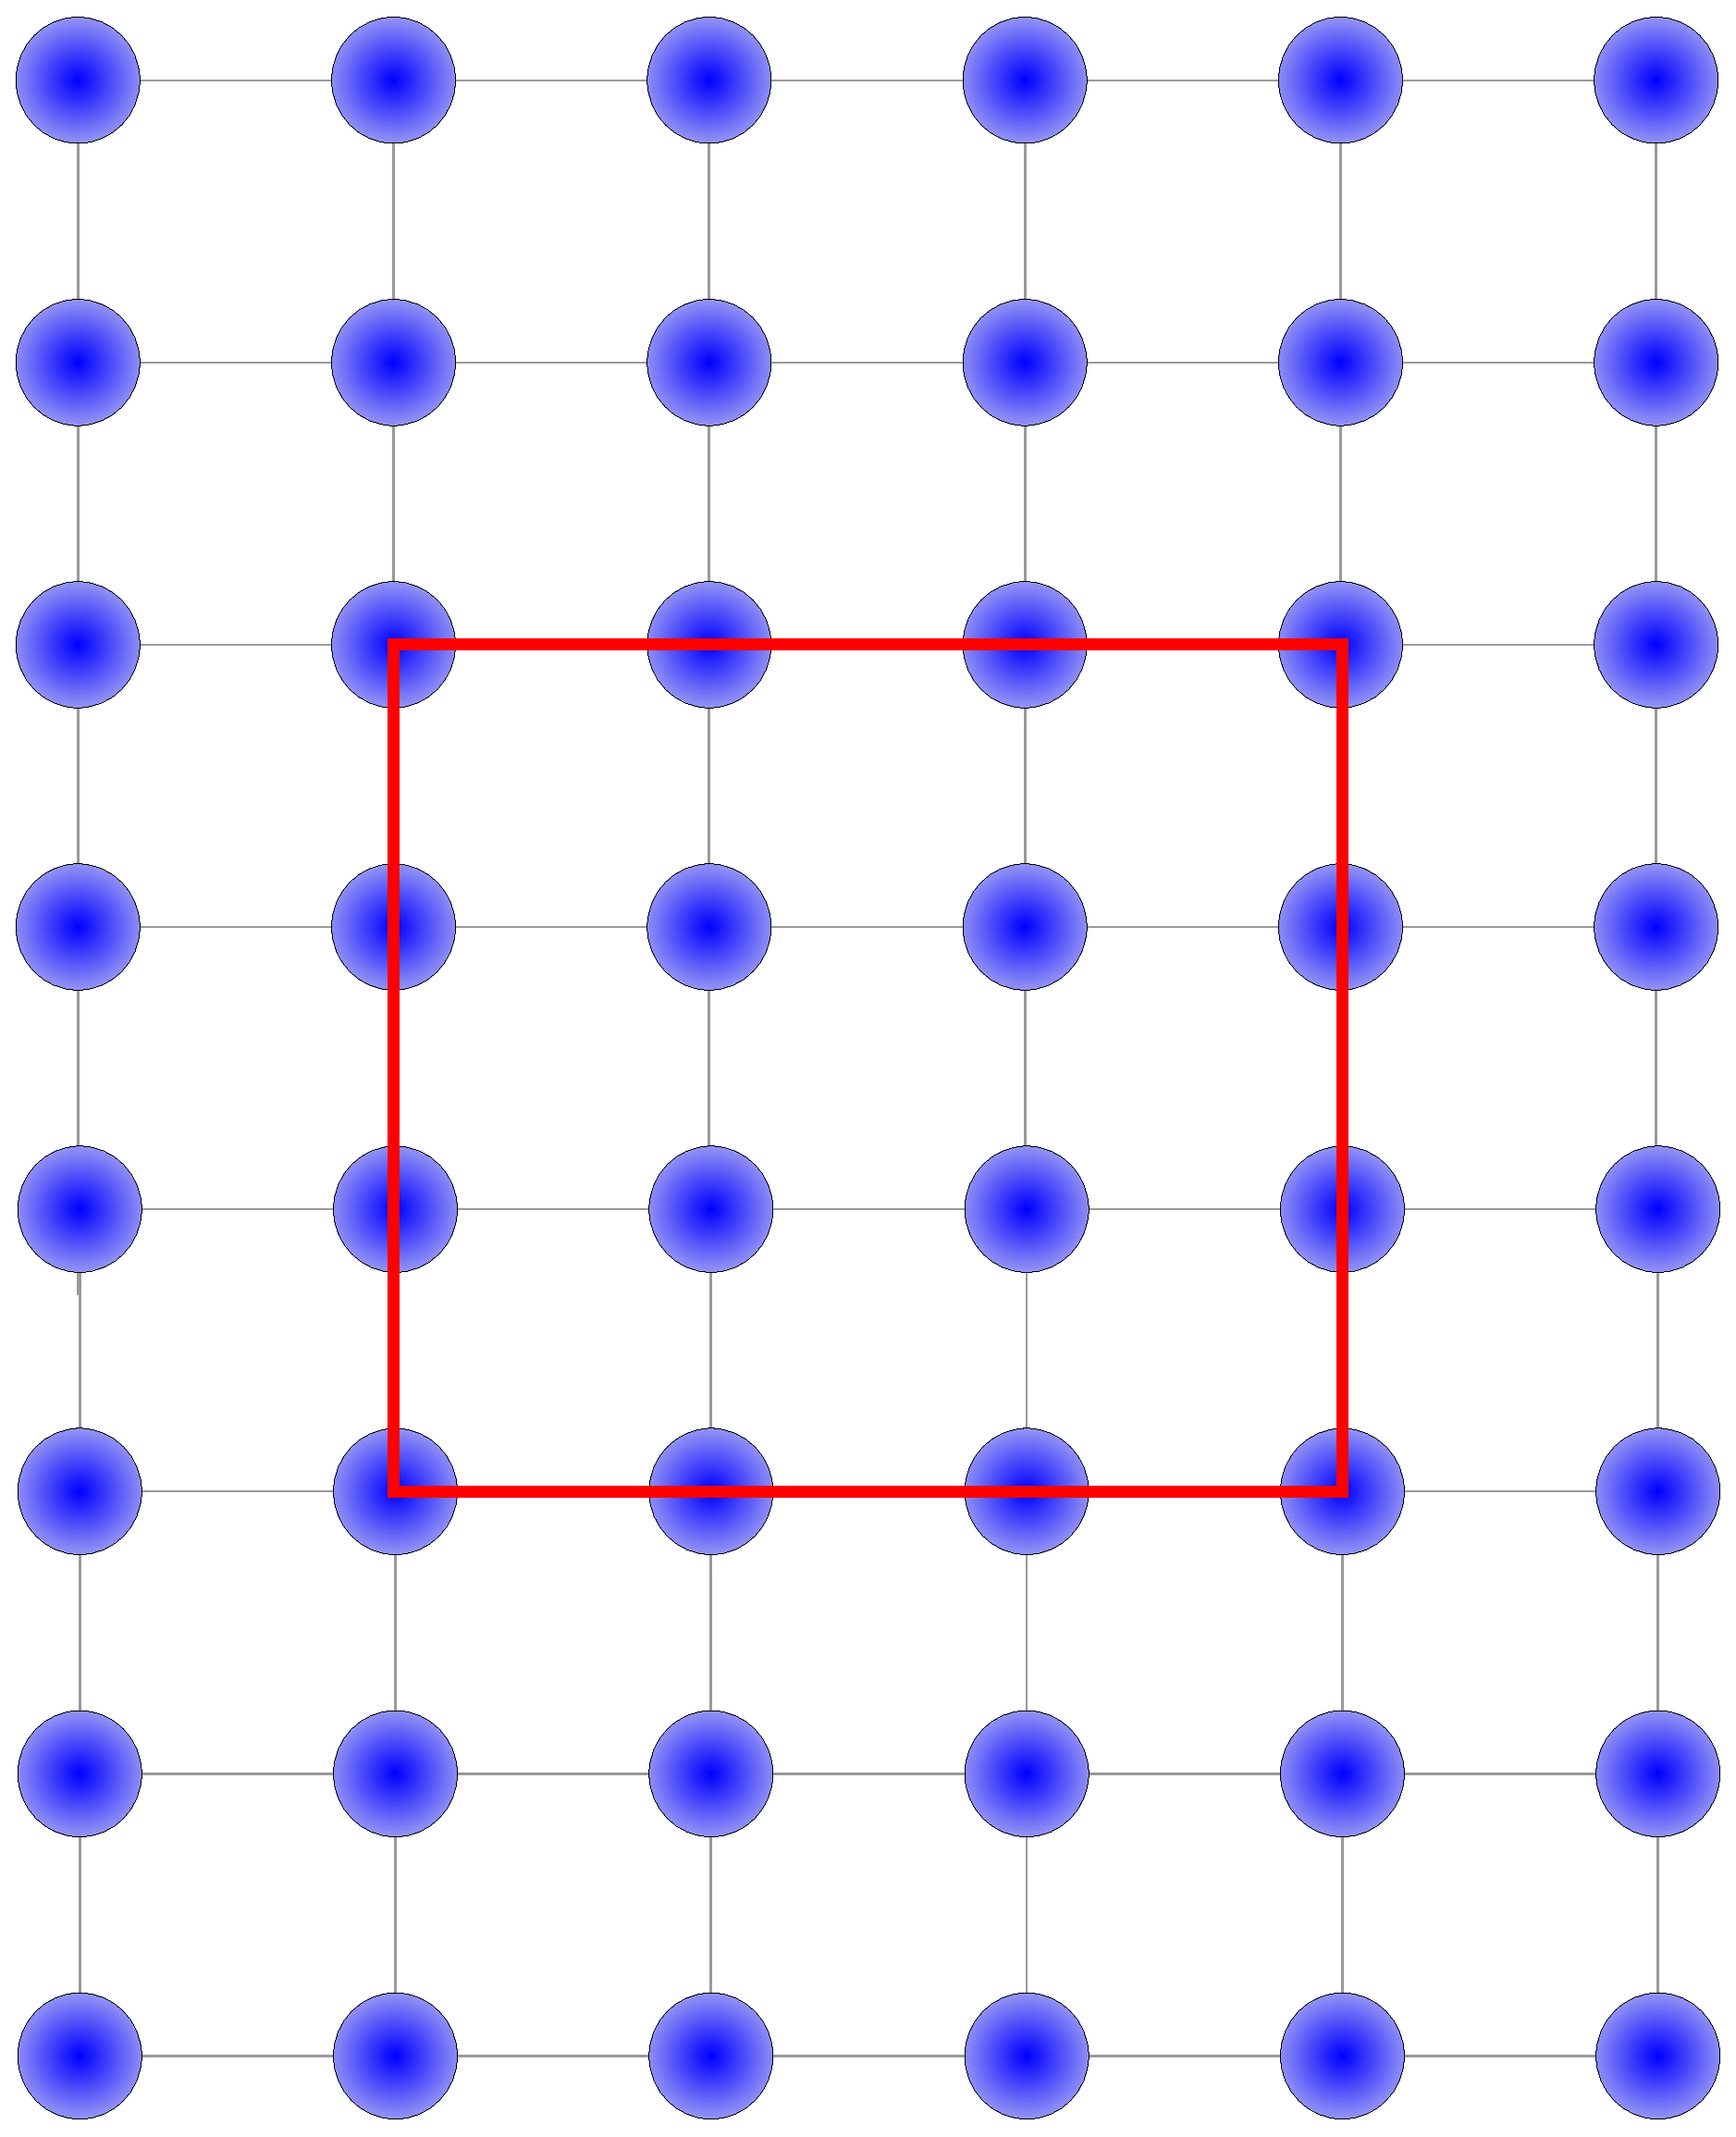
\includegraphics[height=2.5in]{Perfect_crystal_loop}
\caption{A perfect crystal with a complete circuit shown in red.}
\end{subfigure}
\begin{subfigure}{0.4\textwidth}
\centering
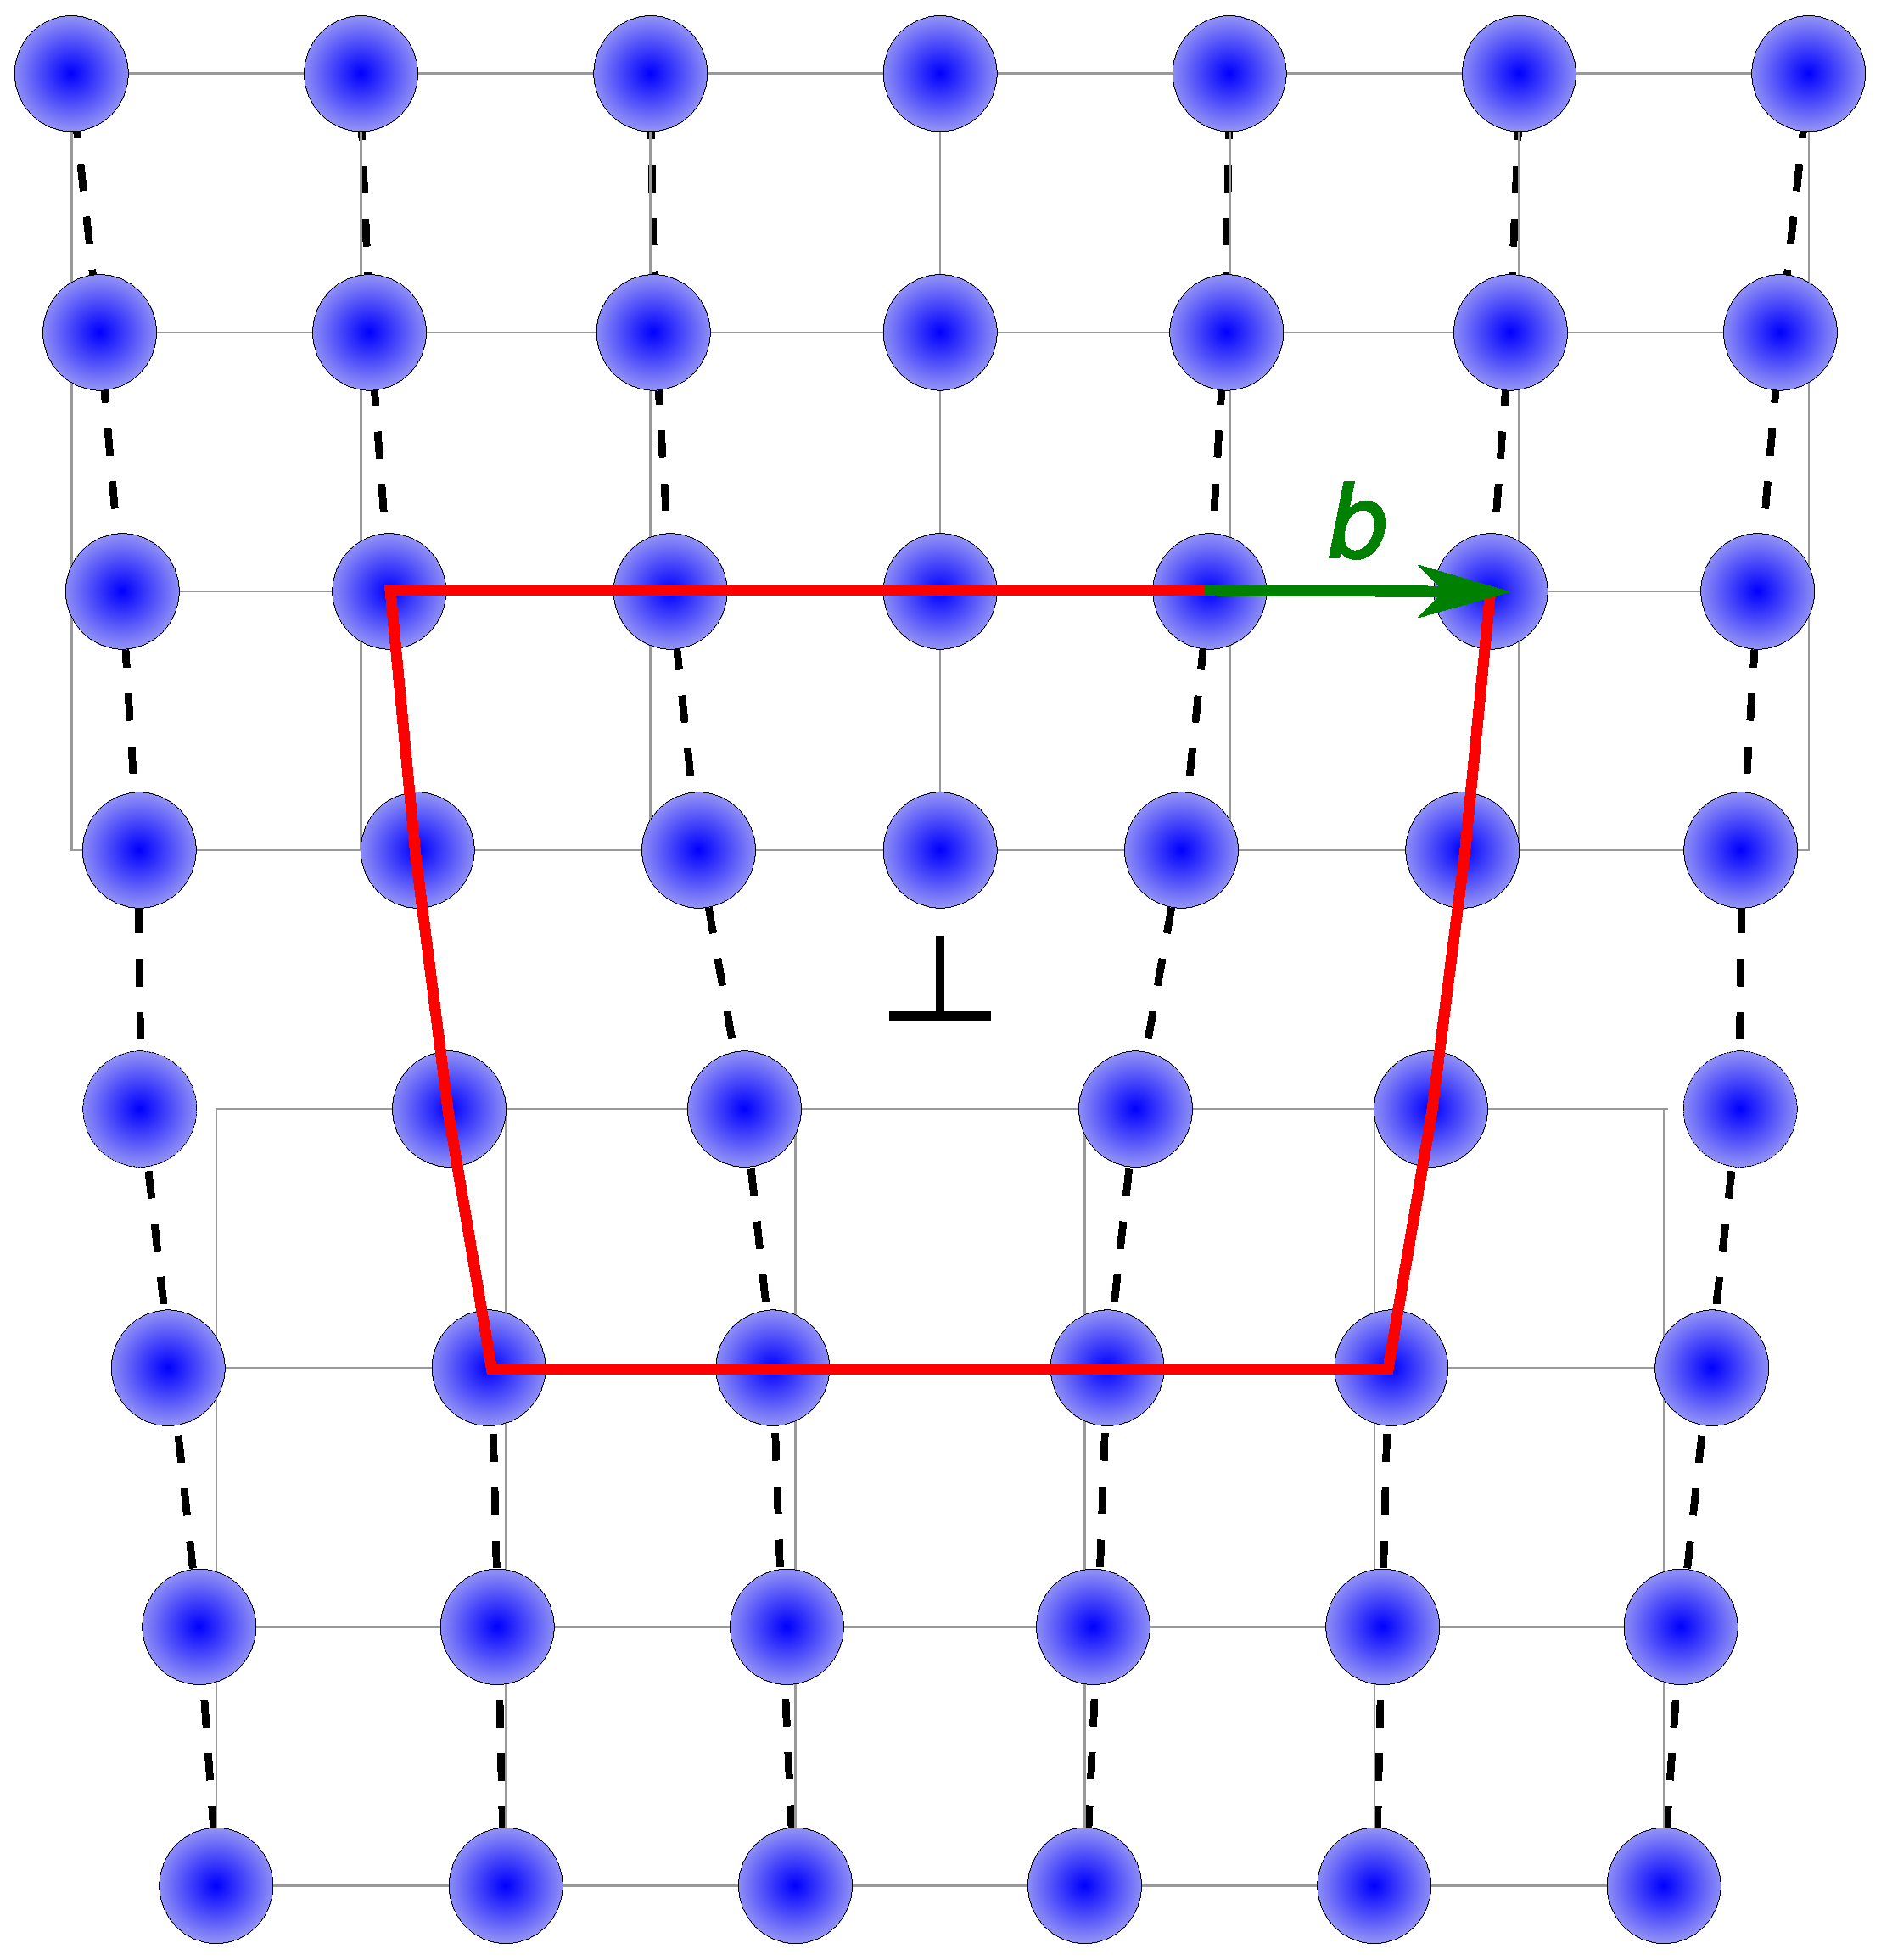
\includegraphics[height=2.5in]{Edge_Dislocation_loop}
\caption{An edge dislocation with an incomplete circuit. \label{fig:Edge_disloc_loop}}
\end{subfigure}

\caption{Inserting a half plane of atoms which terminate in a dislocation and a Burgers circuit to show the Burgers vector. \label{fig:burgers_loops}}

\end{figure}

\begin{figure}
\centering
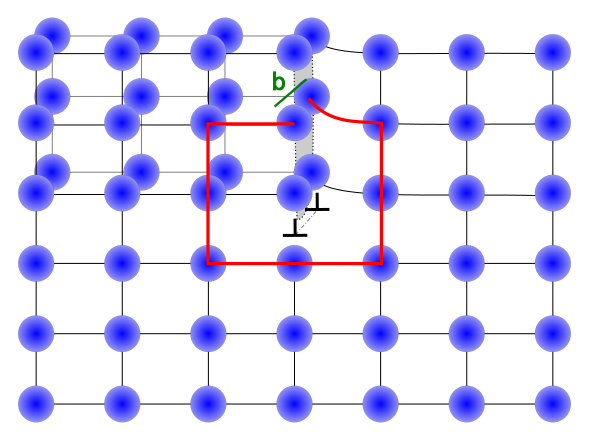
\includegraphics[width=0.7\textwidth]{screw_disloc_loop}
\caption{Schematic of a screw dislocation with a Burgers loop formed in a similar way to \autoref{fig:burgers_loops}. The displacement is parallel to the dislocation line in contrast with edge dislocations. The atomic positions are not relaxed, the displacements being concentrated unphysically into one half plane. \label{fig:screw_disloc}}
\end{figure}




Dislocations can be described in terms of a slip direction, a line direction and a slip plane. The slip direction is simply the direction parallel to the Burgers vector, this is the relative displacement caused by the passage of a dislocation through a region of crystal. The identification of the Burgers vector is done with a Burgers loop, a loop comprised of steps between nearest neighbours is defined that would be closed in a perfect crystal is defined. The same set of steps is undertaken in a dislocated crystal and the loop is no longer closed and the displacement vector between the endpoints is the Burgers vector. This is shown for an edge dislocation in \autoref{fig:burgers_loops}, where the Burgers vector is perpendicular to the line vector, and a screw dislocation in \autoref{fig:screw_disloc}, where the Burgers vector is parallel to the line vector. The line direction can and does vary along the length of the dislocation but is simply the line defined by the defective region of crystal. The slip plane is the crystallographic plane in which the dislocation can move and must contain the slip direction and line direction; where the line and the slip directions are not parallel the slip plane is defined by these two vectors, but for screw dislocations which have the slip direction and line directions parallel the plane is not so constrained, instead the possible slip planes are those that allow easy movement, i.e. lower forces or smaller energy changes, and depending on the crystal symmetry there may be several. This allows screw dislocations to change the plane they are moving in, a process known as cross slip \cite{Hirth_Lothe1982intro}.

Real dislocations are not neat and instead of lining up with convenient crystallographic axes will curve and bend. This usually gives rise to a mixed and varying character of dislocation with the Burgers vector neither parallel nor perpendicular to the line vector. These mixed dislocations are usually described as the sum of edge and screw components.

There are conventions about the sign of dislocations, taking line vectors into or out of the page and defining the sense of Burgers loops and the Burgers vector defined from the finish to the start etc. Given that the symmetry of most of the crystals of interest is high enough to ensure that all these choices are usually arbitrary the only thing that will be highlighted here is that if the sense of a dislocation is reversed then its stress/strain field will reverse in sign. Hence oppositely signed dislocations attract to lower the stored elastic energy and potentially to annihilate line length, while like-signed dislocations will repel to lower the elastic stored energy.



\FloatBarrier

\subsection{Historical overview}


In the early twentieth century there were many observations of real world materials strengths that could not be reconciled with the theoretical shearing strength of a perfect plane of atoms. Indeed for a long time this was neglected because, as \citet{gordon1991} puts it:
\begin{quote}
``Until about 1934 the Establishment explanation of these phenomena was remarkably unconvincing and seems to have reflected mainly a desire not to be asked embarrassing questions.''
\end{quote}

In 1934 the edge dislocation was proposed by \cite{orowan1934i,Orowan1934ii,Orowan1934iii}, \citet{Taylor1934}, and \citet{polanyi1934} to explain the discrepancy between the ideal strength of crystal and the observed strengths of real materials. It was around this time that work undertaken by \citet{Volterra1907} and others, particularly \citet{love1920}
on elastic behaviour of homogeneous isotropic continua was related to plastic flow of crystalline materials, idealised dislocations in elastic continua are termed Volterra dislocations. By the end of the decade \citet{burgers1939} had described screw dislocations. 

It was not until the 1950s that experimental evidence for the existence of dislocations was produced; the initial evidence was growth surfaces of single crystals, preferential etching of a crystalline material at dislocations and x-ray studies of arrays of dislocations in the bulk \cite{Forty1954}. 

\citet{Frank1949} predicted, in 1949, that a step could terminate by the intersection of a dislocation with a free surface, or conversely a dislocation intersecting with a free surface would necessarily create a step; these weere observed soon after in 1950 by \citet{Griffin1950}. Preferenctial etching of dislocations was observed by \citet{horn1952holes} who matched the configuration of etch pits with the pre-existing surface growth features that arise from screw dislocations. The effect of plastic work and subsequent recovery on Laue spots (the xray beams diffracted by a single crystal) provide evidence of arrays of dislocations. The process is described by \citet{Cottrell1949}: Initially sharp Laue spots exist in a perfect crystal. Plastic work smears the spots by introducing a homogeneous distribution of dislocations and the spots then split into distinct sharp spots during recovery as dislocations align into arrays that form sub-grains with small misalignments across the new low angle grain boundaries.


An edge dislocation was first imaged in 1956 by \citet{Menter1956} in platinum phthalocyanine. The large organic complex with a platinum atom at the centre produces widely spaced rows of platinum atoms suitable for imaging with transmission electron microscopy.




\subsection{The stress required to move a dislocation}

Though mathematical descriptions of dislocations in isotropic elastic continua date back to 1907 \cite{Volterra1907} the energies and forces around dislocations in crystalline lattices and the  was not considered until much later. In 1940 \citet{Dehlinger1940} and \citet{Peierls1940}. The former presented the application of the Frenkel-Kontorova model, a one dimensional array of balls connected by springs on a periodic potential/substrate, to approximate a dislocation.

The latter, Rudolph Peierls, was one of the physicists working during the advent of quantum mechanics and most of his work was in that field, however during his education he received a grounding in classical physics at Arnold Sommerfeld's lectures in Munich and so it was that he was suitably equipped when presented with the problem of dislocation motion by Egon Orowan; as Peierls remarked he knew nothing about dislocations but he did know classical elasticity \cite{Edwards1996}.


Peierls presented the first formal solution for the energy changes as a dislocation moves in a rather short note \cite{Peierls1940} and the idea was extended by \citet{Nabarro1947}. The model is remarkably simple; consider two semi-infinite perfect crystals with their lattice aligned but some initial misalignment between them as shown in \autoref{fig:semi_infinite_crystals}. We can join them along what will become the slip plane. An edge dislocation is formed where the energy of the system is lowered by displacing atoms from their initial positions to localise the misalignments around the dislocation core, usually taken to be the origin. I.e. when the energy of a planar defect is higher than that of the linear defect and dislocation will form.



\begin{figure}
\centering

    \begin{subfigure}{0.4\textwidth}
        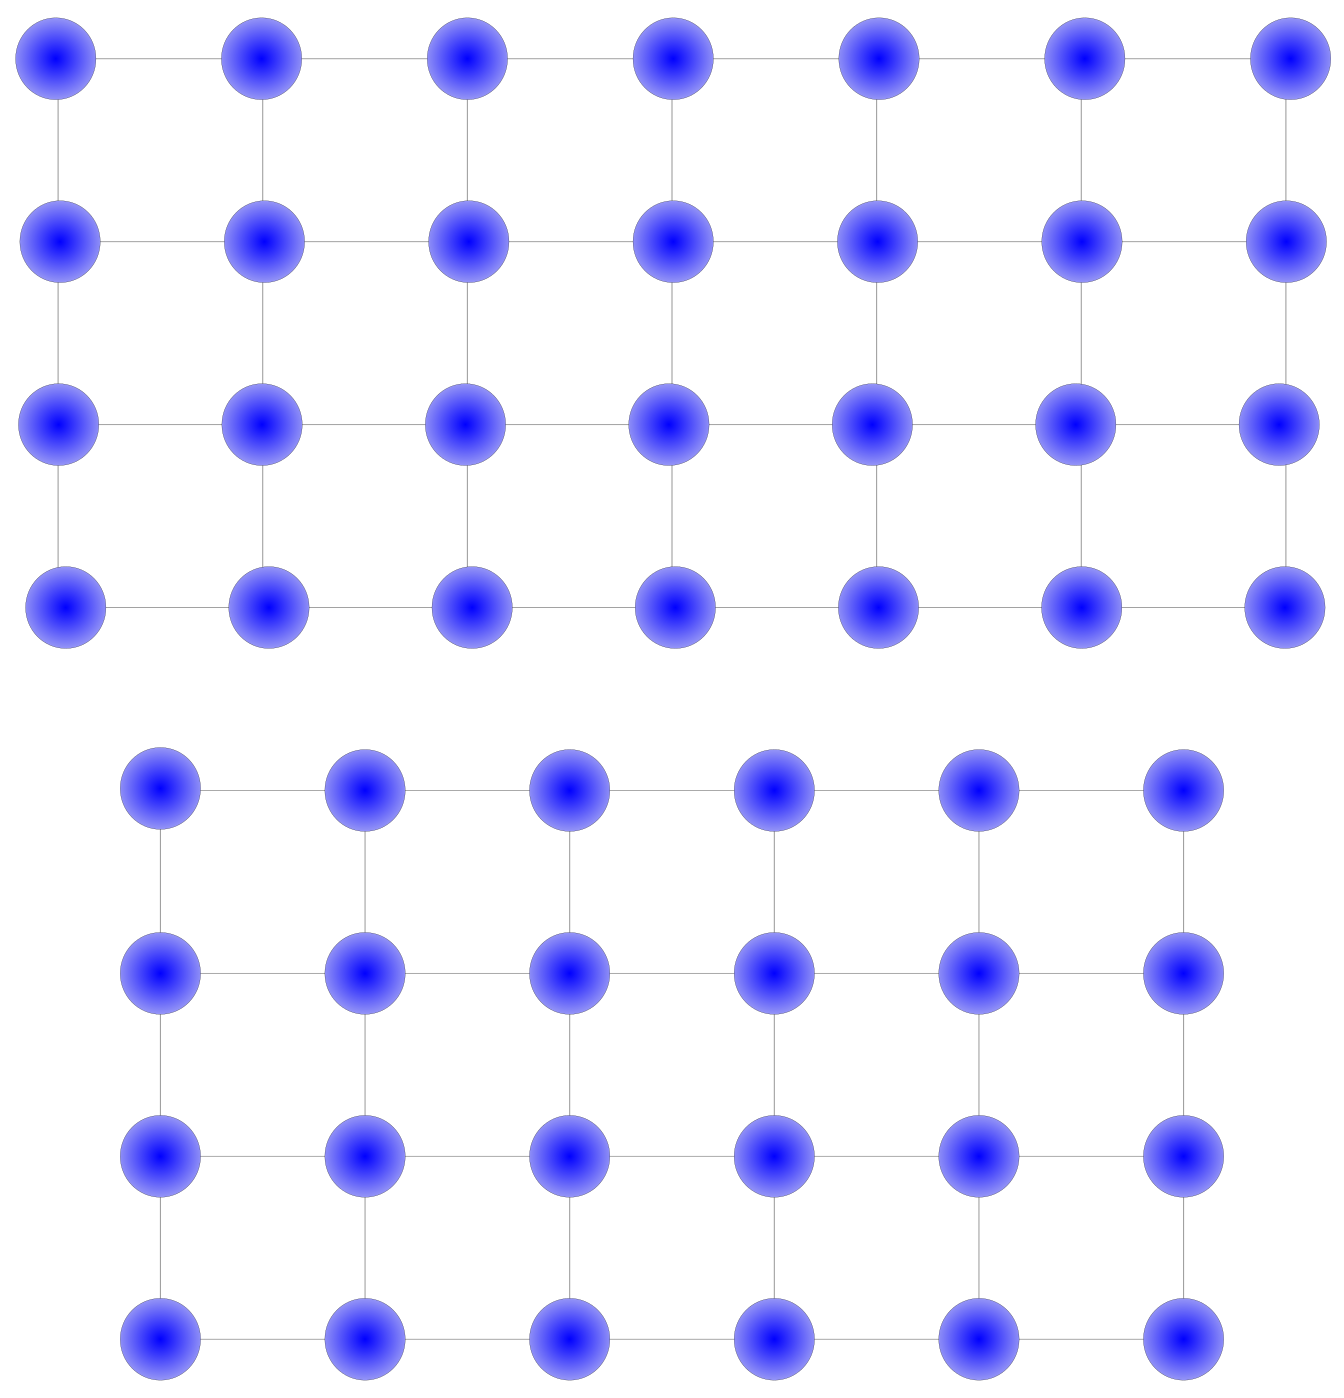
\includegraphics[width=\textwidth]{Half_crystals}
        \caption{Two semi-infinite crystals \label{fig:semi_infinite_crystals}}
    \end{subfigure}

    \begin{subfigure}{0.4\textwidth}
        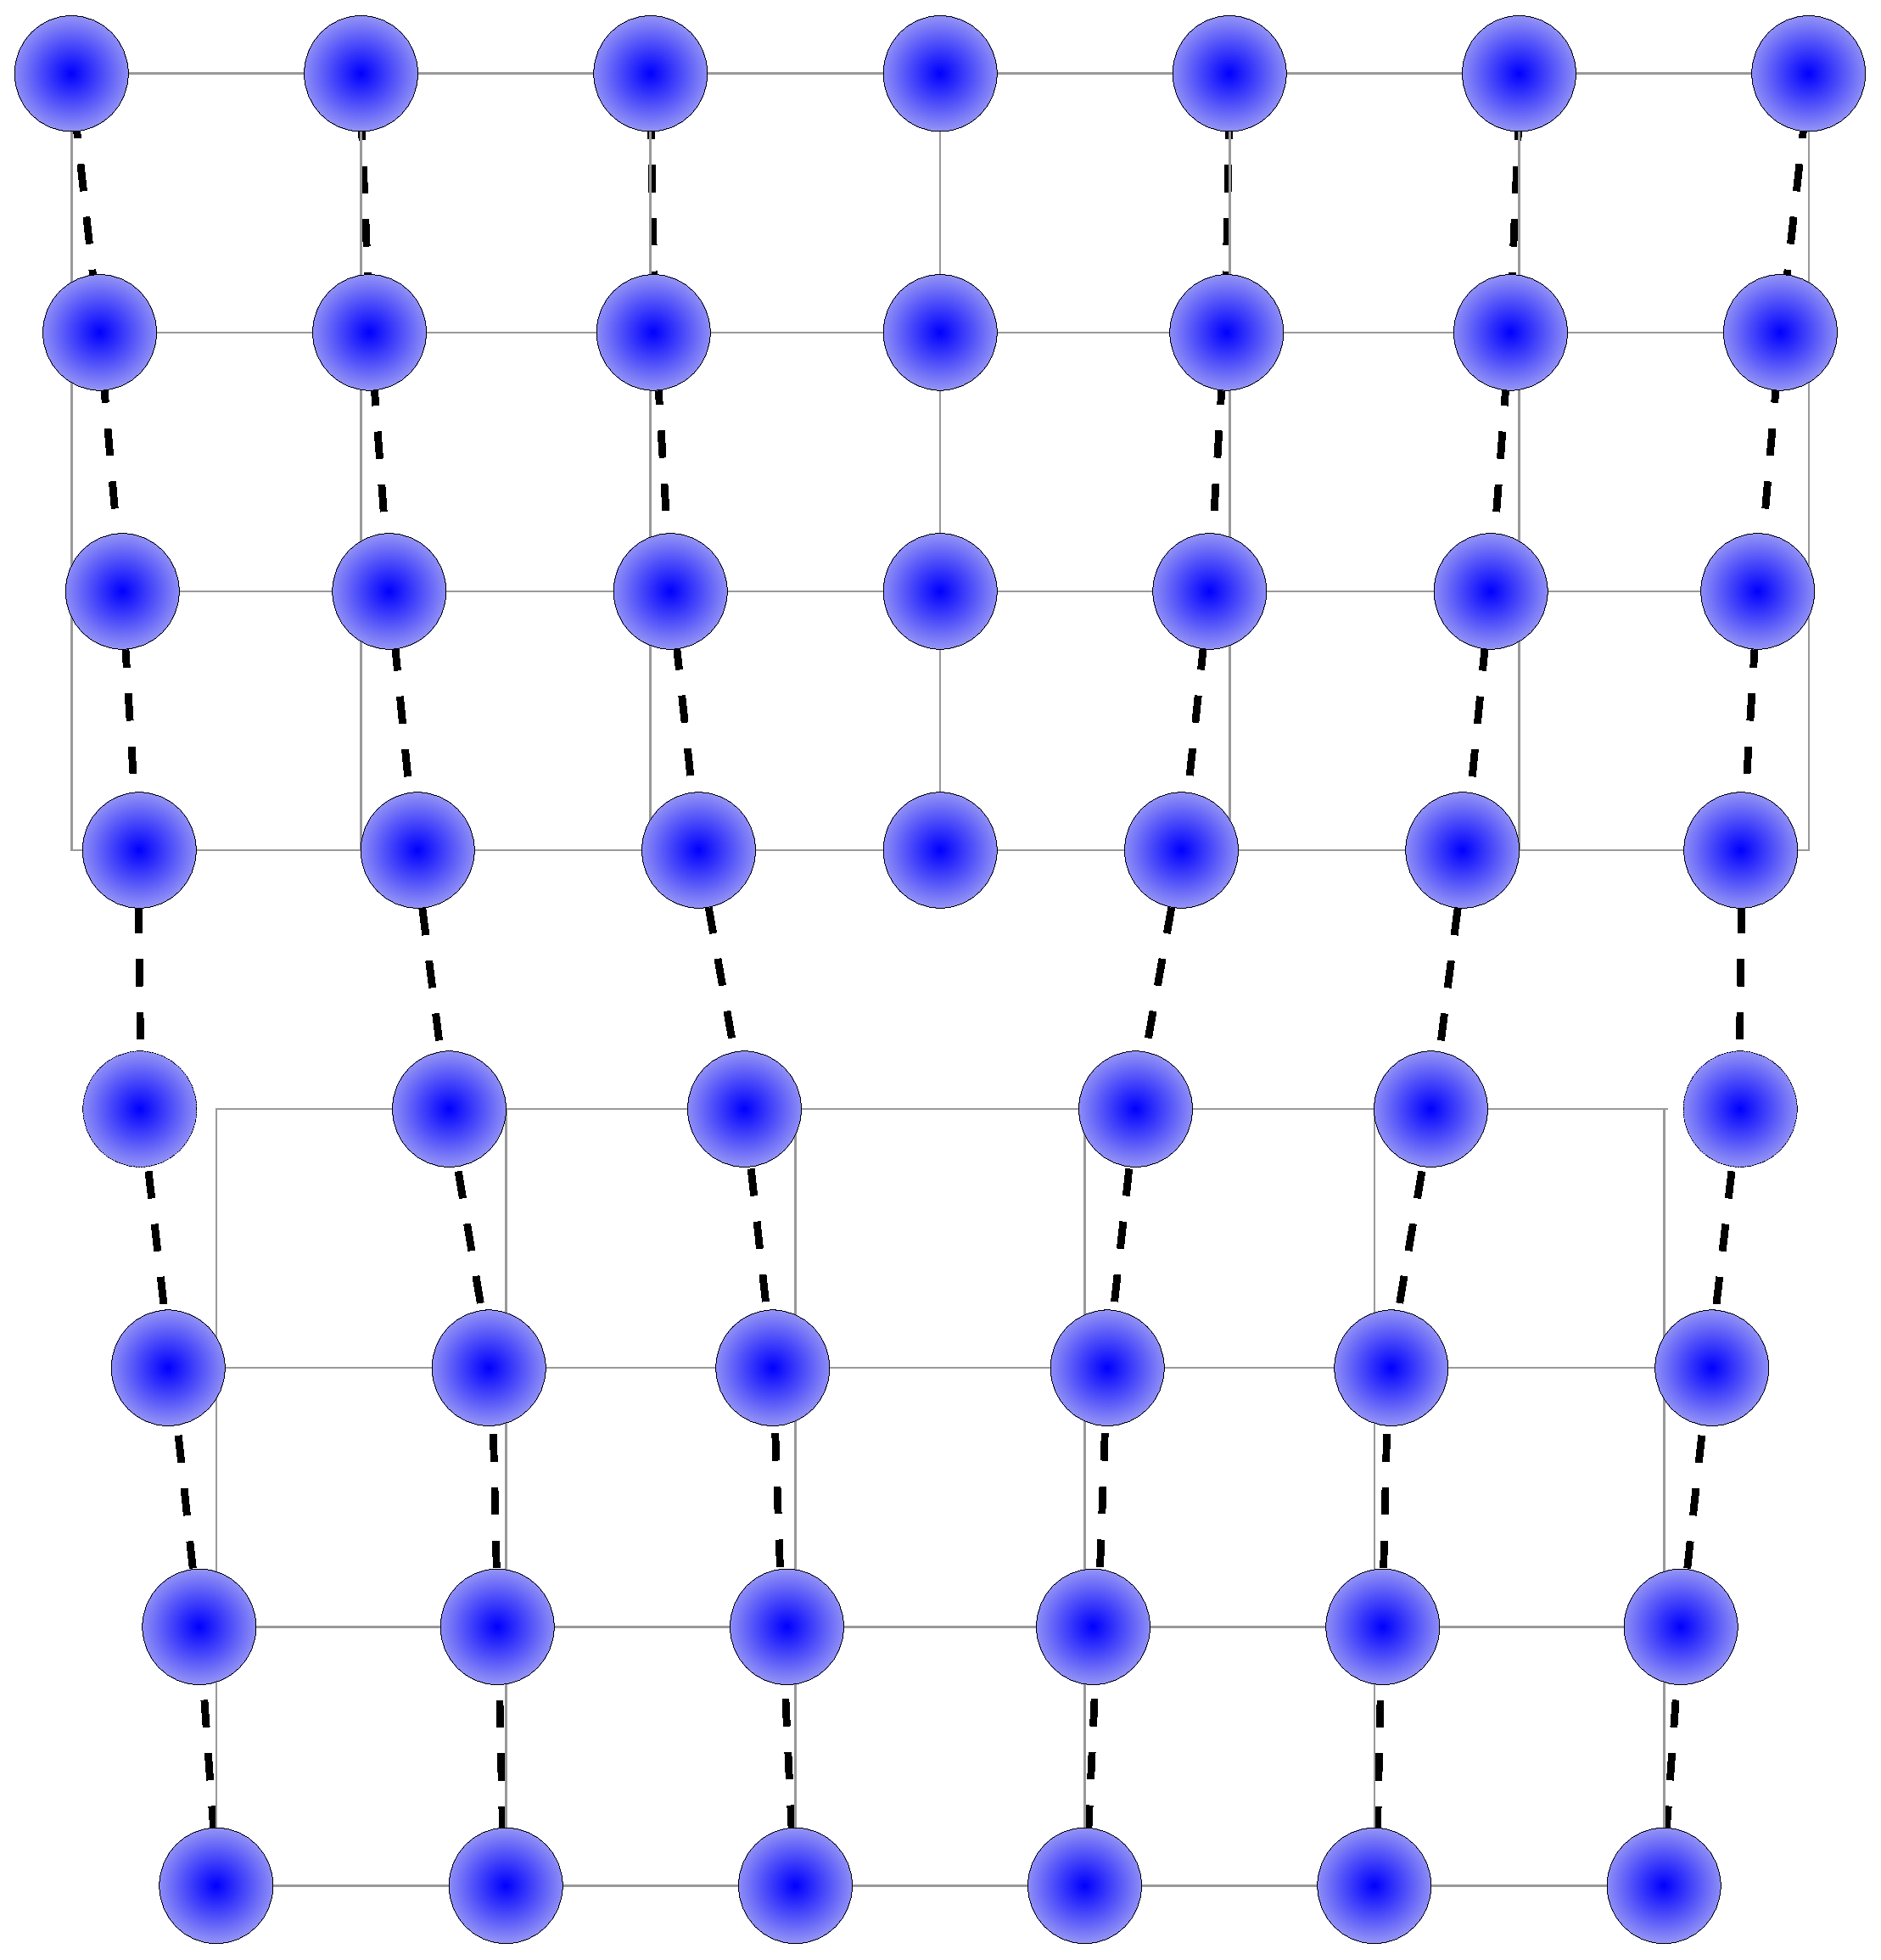
\includegraphics[width=\textwidth]{Edge_Dislocation}
        \caption{A schematic edge dislocation\label{fig:joined_half_crystals}}
    \end{subfigure}

    \caption{Schematics showing the creation of an edge dislocation in a simple square lattice by the joining of two misaligned half crystals. \label{fig:edge_disloc}}
\end{figure}

\begin{figure}
\centering
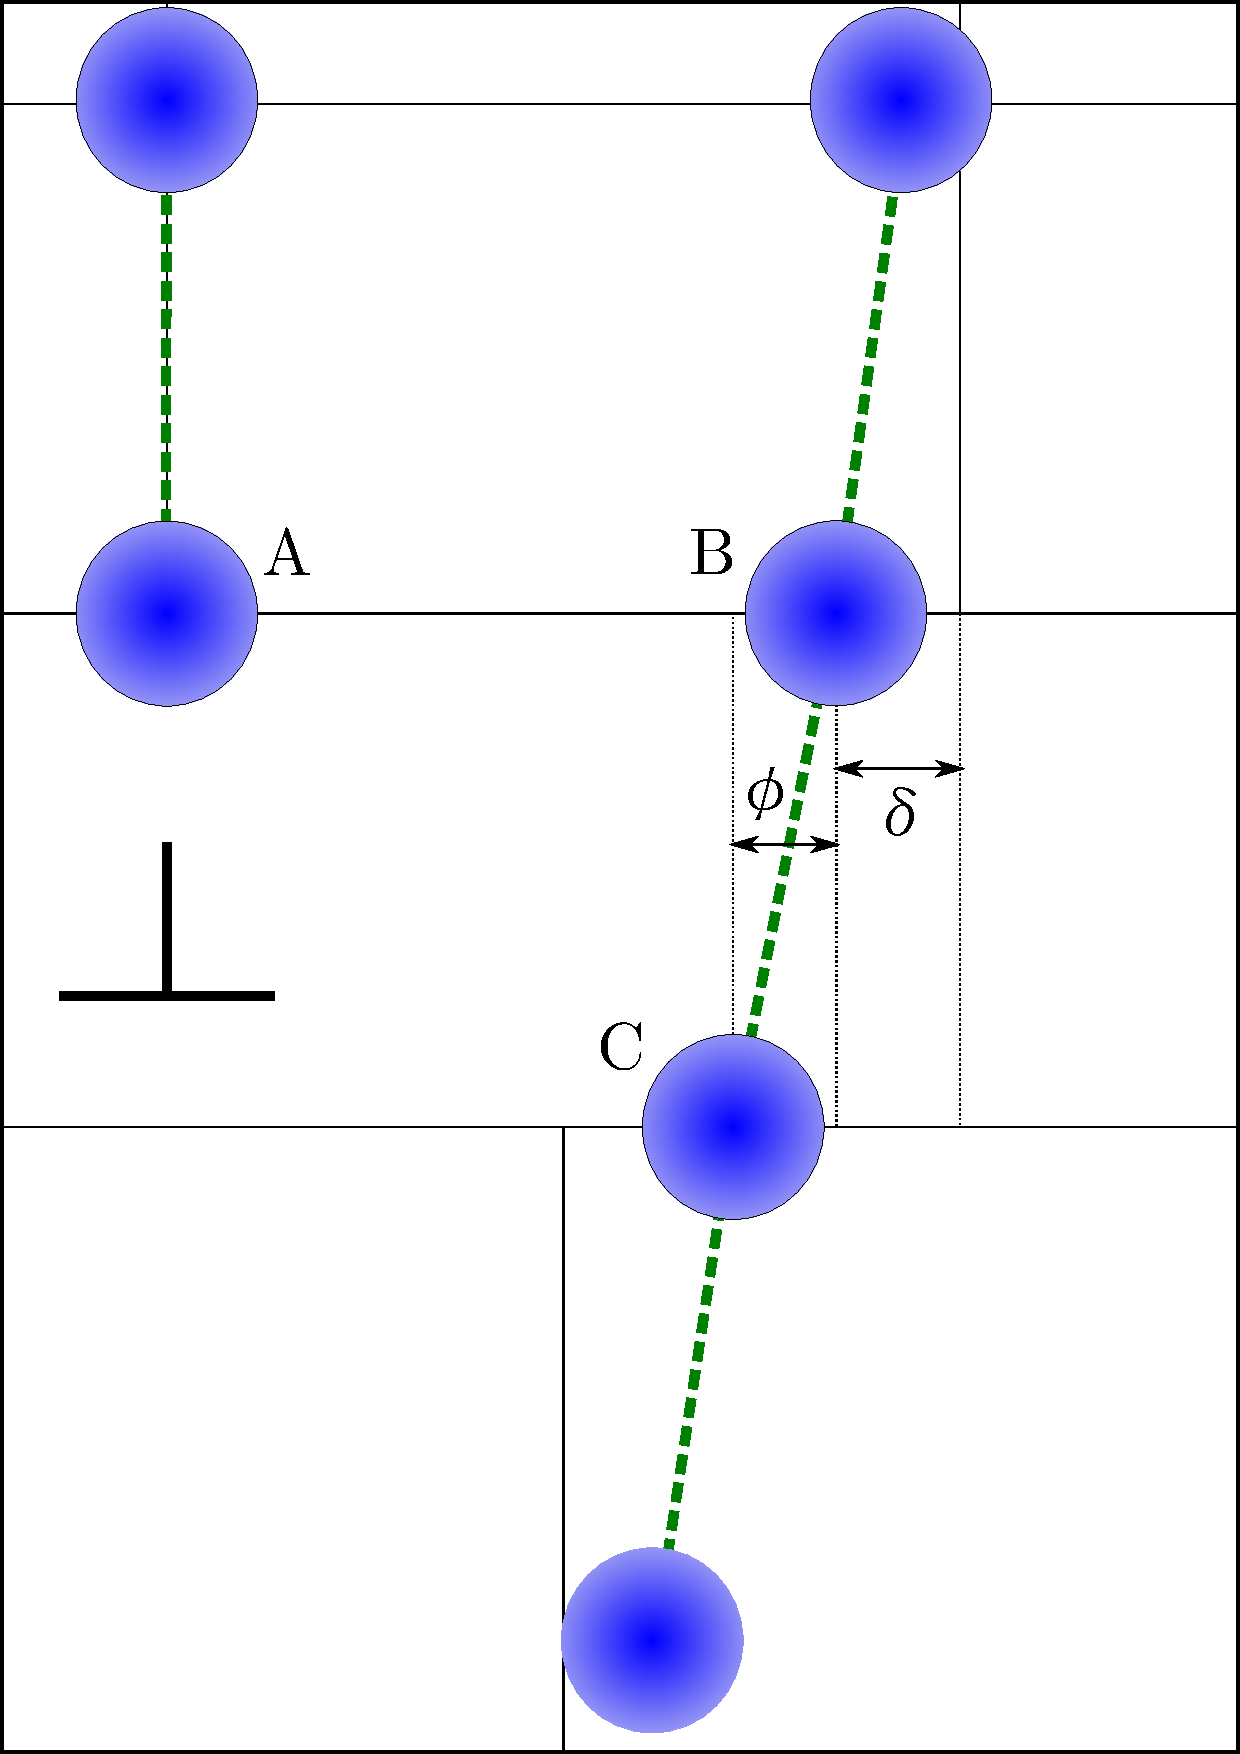
\includegraphics[width=0.6\textwidth]{peierls_model_detail}

\caption{Detail of the local displacements around the dislocation core. $\delta$ is the extension of the bond parallel to the slip plane between atoms A and B, while $\phi$ is the misalignment of the bond across the slip plane between B and C.\label{fig:detail_of_peierls}}
\end{figure}

Atomic configurations that form a dislocation are generated by by applying a displacement field to the atoms immediately above and below the slip plane, $u(x)$ and $u'(x)$ respectively. The Peierls model then estimates the energy of the configuration by considering two restoring forces generated by the atomic arrangement. The detail is show in \autoref{fig:detail_of_peierls}. Firstly the bonds parallel the slip plane will be either extended or contracted, for example the bond between atom $A$ and $B$ has been contracted by the amount $\delta$, this will tend to oppose the concentration of misalignments to the core and is zero in the case of no displacements from the initial positions. Secondly the misalignment of bonds across the slip plane, the bond between atom $B$ and $C$ is misaligned by a lateral distance of $\phi$. This misalignment energy will tend to favour the concentration of the misalignments to the core and is a maximum in the case of no displacement from the initial position.

Peierls made the assumption that the displacements vary slowly with position, i.e. that the dislocation is very wide. This means that the strain in the slip plane (i.e bonds like $\overrightarrow{AB}$ in \autoref{fig:detail_of_peierls}) experience only small strains. The energy associated with these \emph{in-plane} strains are then described  by the application of the displacement field to the surface of two semi infinite elastic continua. 
The \emph{misalignment} energy of bonds across the slip plane (bonds like $\overrightarrow{BC}$ in \autoref{fig:detail_of_peierls}) is assumed to be a periodic function, specifically a simple sinusoidal variation is taken to be the form of the misalignment potential:

\begin{equation}
U_{mis} = C \sin \left(\frac{2\pi [u(x) - u'(x)]}{d} \right)
\end{equation}













%%%%%%%%%%%%%%%%%%%%%%%%%%%%%%%%%%%%%%%%%%%%%%%%%%%%%%%%%%%%%%%%%%%%%%%%%%%%%%%%%%%%%%


%
%
%
%
%   Sort out this Frenkel stuff
%
%
%
%
%
%


%%%%%%%%%%%%%%%%%%%%%%%%%%%%%%%%%%%%%%%%%%%%%%%%%%%%%%%%%%%%%%%%%%%%%%%%%%%%%%%%%%%%%%



The constant, $C$, has to be chosen appropriately but can be found by assuming linear elasticity holds at small strains. \citet{Frenkel1926} derived a similar sinusoidal function for the stress to form a stacking fault:










\begin{equation}
\tau_{fault} = \tau_{\text{theory}} \sin \left( \frac{2\pi \phi}{b} \right)
\end{equation}

The energy of the dislocation is the sum of all these contributions. There will be a configuration that is a minimum in the total energy where the in-plane forces widening the dislocation balance the misalignment forces that drive it to be narrower. This gives rise to a size, or width, of a dislocation. The width of the dislocation is defined as the distance from the core at which the misalignment across the slip plane is half its maximum. Peierls calculated this for an isotropic elastic solid and accounting for only the atomic planes immediately adjacent to the slip plane and found it to be 

\begin{equation}
w = \frac{d}{1-\nu}
\label{eqn:width_isotropic}
\end{equation}
where $d$ is the plane spacing across the slip plane and $\nu$ is the Poisson ratio.

The stress required to move a dislocation can be calculated from the maximum energy \emph{gradient} as the dislocation is displaced. Since the in-plane strains have a continuous definition in this model the displacement of the dislocation has no effect and the in-plane strain energy does not change. The energy changes therefore depend only on the misalignment energy of bonds across the slip plane and the energy of all the atoms away from the slip plane re neglected.

Peierls gave the critical stress, the \emph{Peierls Stress}, for an isotropic elastic material in terms of the ideal shear strength as calculated for uniform slip and accounting for only the interactions between the first plane either side of the slip plane, as


\begin{equation}
\frac{\tau_p}{\tau_{ideal}} = \frac{4 \pi}{1 - \nu} (5.8 - \log|1-\nu|) \exp\left(-\frac{4\pi}{1 - \nu}\right).
\end{equation}

This was refined by \citet{Nabarro1947} and the direct summation of the discrete contributions was developed by Cottrell and Nabarro \cite{Cottrell1953}. The result of that summation is



\begin{equation}
\tau_p = \frac{2\mu}{1-\nu} \exp\left( - \frac{4\pi w}{b} \right)
\end{equation}
where $\mu$ is the shear modulus and $b$ is the burgers vector.

For an isotropic material the width can be substituted from \autoref{eqn:width_isotropic}:

\begin{equation}
\tau_p = \frac{2\mu}{1-\nu} \exp\left( - \frac{2\pi d}{(1-\nu)b} \right).
\end{equation}

Although this simple model includes some large assumptions the method moved dislocation theory on in two ways: firstly continuum elasticity could not account for energy changes as the dislocation moves since in an isotropic homogeneous continuum one dislocation position is identical to all others and there will be no energy changes as the dislocation move, and secondly this approach removes the singularity at the core predicted by continuum elasticity for Volterra dislocations.


An important point to note is that the Peierls stress is extremely sensitive to the size of the dislocation, $w$, and therefore to the factors that control the width; which in turn is defined by the lattice geometry, $d/b$, and the elastic properties.



Peierls found the perhaps surprising result that the energy changes have a periodicity of $b/2$ rather than $b$, this has been ascribed to the summation procedure of the energy of the misaligned bonds across the slip plane, of which there has been much discussion \cite{Hirth_Lothe1982lattice_periodicity,Lu2000peierls}. Peierls summed over the atoms above the slip plane and below the slip plane independently, the ``double-counting'' scheme, later models used a ``single-counting' scheme in which the assumption of small displacements is dropped and the misalignment of an atom above the slip plane is dependent on the final position of the atoms below the slip plane. This is given as the reason the Peierls barrier had a wavelength of $b/2$ rather than $b$ \cite{Hirth_Lothe1982lattice_periodicity,Lu2000peierls} though it has been suggested that the problem is an artefact that arises from an assumption of small displacements and that using the final rather than initial positions of the atomic rows resolves the difficulties \cite{Huntington1955}. There is another explanation for the change in period that depends on the exact formulation of the energy calculations and whether the $\alpha=1/2$ position is symmetrically equivalent to the $\alpha = 0, 1$ positions. The periodicity of $b/2$ is easily explained on this basis because Peierls assumed that both the elastic energy and the dislocation geometry remained constant and the only changes in the energy were therefore based on misaligned bonds across the slip plane. These assumptions produce an atomic configuration at $\alpha=1/2$ that is the a reflection  of the $\alpha=0$ configuration across the slip plane, which must give the same energy since the misalignment potential used by Peierls is symmetrical.




There have been many criticisms of and modifications to the Peierls model in the years since but these have largely focused on adjusting the assumptions of the original method.
In 1951 \citet{Foreman1951} introduced phenomenological potentials to describe the energy of the misaligned interactions across the slip plane, they discovered that the width of the dislocation was predicted to be larger than that of the original treatment and was coupled with a decrease in the Peierls stress.

In 1955 \citet{Huntington1955} modified the model to double the periodicity and so account for crystals in which a displacement of half a burgers vector is not symmetrical with no displacement, or in other words broke the mirror symmetry of the slip plane. 
\citet{Maradudin1959} considered a completely atomistic three dimensional model of a screw dislocation but did not consider radial displacements. That work only evaluated the energies of the symmetric and anti-symmetric configurations and so only estimated the energy change, not the maximum stress.



In 1994 a fully discrete model was developed by \citet{Ohsawa1994}. This model made similar assumption to the original Peierls model in that the only energy changes were in the sheared misaligned bonds across the slip plane but instead of solving for an analytical solution Ohsawa et al. used numerical methods to optimise the configuration of 84 atoms,  either side of the dislocation core. The model made no assumptions about the displacement field and instead iteratively improved all the atomic positions to find the equilibrium configuration. This was done for increasing applied external stresses until there was no stable configuration, at which point slip would occur.





The generalised stacking fault (GSF) energy or $\gamma$-surface was incorporated into the Peierls model by \citet{Vitek1992} and this was extended by \citet{Bulatov1997}. This addresses a fault in the original Peierls formulation that the sinusoidal potential used to calculate the misalignment energy is too high and steep. \citet{Ohsawa1994} had already attempted to address this by using alternative potentials, but they were essentially arbitrary functions that fitted the shear modulus at small strains instead Bulatov et al. retained the variational approach but used density functional theory (DFT) calculations to generate a misalignment potential, extending the model to include a three dimensional potential to allow both lateral and vertical displacements of the atoms in the slip plane. This is important around the core where large strains mean that the energy contributions are very inaccurate. By using the DFT to calculate the misalignment potential the Peierls model can bridge the length scales between the large scale stress and strain fields around the dislocation and the large local displacements at the core. This is no longer analytically solvable but is not difficult to solve numerically, the only limit being computational time.

Analytical approaches have continued, \citet{Joos1997} developed a closed form solution that was valid for narrow dislocations, where as the original model relied on the assumption of a wide dislocation for simplicity, and achieved a significantly better agreement with experiment than the original formulation. The model proposed by Joós and Duesbery required input parameters calculated by empirical or ab initio methods but used these as parameters of a closed form solution, in particular they required the maximum restoring stress for the glide plane, i.e. the maximum gradient of the GSF energy.

\begin{figure}
\centering
\begin{subfigure}{0.4\textwidth}
\centering
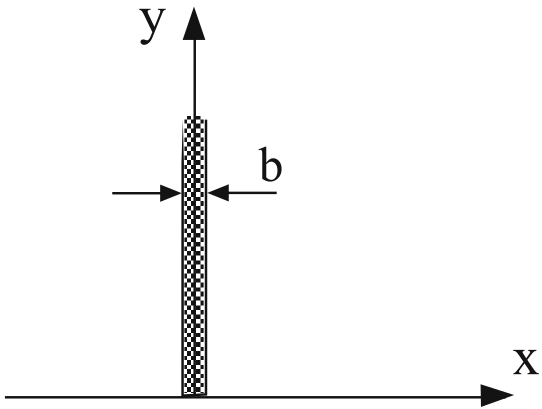
\includegraphics[width=0.75\linewidth]{Dislocation_with_discontinuity}
\caption{Volterra dislocation.\label{fig:disloc_discontinuity}}
\end{subfigure}%
\begin{subfigure}{0.4\textwidth}
\centering
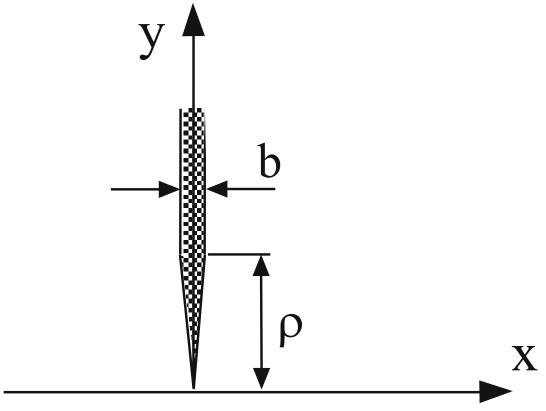
\includegraphics[width=0.75\linewidth]{Dislocation_without_discontinuity}
\caption{Lubarda dislocation\label{fig:disloc_no_discontinuity}}
\end{subfigure}
\caption{The displacement discontinuities in the traditional Volterra dislocation and that used by Lubarda and Markenscoff that removes the singularity at the core. From \cite{Lubarda2007}\label{fig:discontinuity}}
\end{figure}

A continuum elasticity solution was presented by \citet{Lubarda2007} which removed some of the limiting assumption of the original Peierls model, notably the assumption of fixed dislocation geometry as the dislocation was translated from one symmetrical position to the next and that only the misfit energy of the slip plane changes and that the elastic energy away from the slip plane remains constant. The main challenge to using continuum elasticity to solve the Peierls model directly is the singularity in stress and strain at the dislocation core. 
This singularity arises where the displacement discontinuity of a Volterra dislocation across the half plane of an edge dislocation terminates at the core shown in \autoref{fig:disloc_discontinuity}. 
By introducing a gradual increase in the displacement discontinuity across the plane of an edge dislocation from zero at the core to $b$ at some finite distance, as shown in \ref{fig:disloc_no_discontinuity}, Lubarda and Markenscoff were able to formulate a tractable linear elastic continuum problem which produced much better agreement than previous analytical solutions. They found this distance to be be interpretable as the width of the dislocation giving rise to displacements that are consistent with the original Peierls model. 



In 2006 \citet{Clegg2006} used an atomistic approach to the strains outside of the slip plane in addition to the energy of the misalignment across the slip plane. The atomic displacements were taken to have the same form as Peierls had derived, that is

\begin{equation}
u(x_0) = \pm \tan^{-1}\frac{x_0}{w}.
\end{equation}

where $x_0$ is the initial coordinate in the dimension parallel to the burgers vector and $w$ is the dislocation width, now a parameter to be optimised with no closed form solution. The misalignment energy was taken to be

\begin{equation}
U^{x} = \frac{Gb^3}{4\pi^2 d} \sum_n \left[ 1 - \cos \left(\frac{2\pi \phi_n}{d} \right)\right]
\end{equation}
 
 and the in-plane strain energy was taken to be 
 
 \begin{equation}
 U^i = \frac{E}{2(1-\nu^2)} (b\cdot d) \sum_n \epsilon_n^2
 \end{equation}

where $G$ is the shear modulus of the material, $E$ is the Young's modulus, $\nu$ is the Poisson ratio, $b$ is the Burgers vector, $d$ is the slip plane spacing, $\epsilon$ is the strain and is calculated by $\epsilon = \delta/b$, $\delta$ is the extension of an in plane bond and $\phi$ is the misalignment of the bond across the slip plane. $\phi$ and $\delta$ are shown in \autoref{fig:detail_of_peierls}. The energies are then summed over interaction between atomic rows extending 1000 atomic spacings either side of the dislocation core.

The width no longer has an analytical solution so must be found numerically. The variation of the energy was shown to be smooth and have only one minimum because the misalignment energy is monotonically increasing with increasing width and the elastic in plane strain energy is monotonically decreasing.

It is interesting to note that this formulation restores the symmetry that is destroyed in the calculation of elastic energy by continuum elasticity in that the strains above and below the slip plane are symmetric. So despite allowing the strain energy to vary as the dislocation moves this model has the same period as the original Peierls model of $b/2$.





\section{Ductility criteria}
\label{sec:ductility_criteria}



In most structural applications a catastrophic brittle failure by fast fracture is unacceptable. Furthermore many materials used in devices or coatings both protective and functional often fail by brittle fracture and so a material that is more ductile, at least relatively, may have improved performance. This has motivated numerous attempts to find ductility criteria to predict from simple and easily measurable properties whether a material will fail in a ductile or a brittle manner.

The Pugh ratio, $B/G$ where $B$ is the bulk modulus and $G$ is the shear modulus, is one of the most widely known and is still used today \cite{Sangiovanni2011,Aryal2014,Wang2015,Hu2016,Zhuang2017}. This ratio is used to indicate the relative ease of either plastic deformation or brittle fracture. High values of this ratio should tend to indicate ductility while low values should indicate brittleness. This can be physically justified on the basis that the resistance to slip is proportional to the shear modulus: as Pugh discussed, the Orowan bowing stress is proportional to $G$, but it can also be justified from the lattice resistance, which is also proportional to $G$, see \ref{eqn:Peierls_Stress}. For a given lattice, i.e.\ constant $d/b$, the shear flow stress should scale with the shear modulus. In a similar way, the ease of fracture must be related to the ease of separating layers of atoms. Since this must relate to the energy of straining bonds and the energy of creating surfaces, Pugh took the bulk modulus is a reasonable proxy. This gave good results empirically when \citet{Pugh1954} analysed a wide range of material data.

However this does not accurately capture reality. For example for two face-centred cubic metals, aluminium and copper, $B/G$ is 2.74 and 3.00 respectively, and these metals both show large elongations to failure. For Rhodium and Iridium, $B/G$ is 1.77 and 1.74 respectively, and they show small elongations to failure \cite{Pugh1954}. On the other hand very brittle phases are easily found with similar values of $B/G$; the C15 Laves phases \cite{Stein2004,Stein2005} \ce{NbCr2} and \ce{HfV2} have large values of $B/G$, 2.88 and 3.47 respectively \cite{Chu1995}, but exhibit no significant plasticity whatsoever. In contrast \ce{Ti3SiC2} has a value of $B/G$ of 1.37 (using experimental polycrystalline values) \cite{Barsoum2011} and shows very easy slip.



%%%%%%%%%%%%%%%%%%%%%%%%%%%%%%%%%%%%%%%%%%%%%%%%%%%%%%%%%%%%%%%%%%%%%%%%%%%%%%%%%%%%%%%%%%%%%%%
% Maybe the graph of $B/G$ ratios for fcc metals and Laves phase here
%%%%%%%%%%%%%%%%%%%%%%%%%%%%%%%%%%%%%%%%%%%%%%%%%%%%%%%%%%%%%%%%%%%%%%%%%%%%%%%%%%%%%%%%%%%%%%%



\citet{rice1974} suggested an alternative approach based on the energetics of sharp crack tips and whether blunting dislocations can be spontaneously emitted. The analysis used the Peierls approach to evaluate the energy of a dislocation close to free surfaces and found that the term $Gb/\gamma_s$, where $\gamma_s$ is the surface energy, $G$ is the shear modulus and $b$ is the Burgers vector, to be a dimensionless value that reflects the propensity to fail by either ductile or brittle means and is justified along similar lines to the Pugh ratio. $Gb$ scales with the energy of emitting a blunting dislocation, so high values will oppose the formation of dislocations and blunting of cracks, thus favouring brittle failure. On the other hand $\gamma_s$ represents the energy of the crack and high values will tend to favour reduction of the surface by blunting and favour ductile failure. 

The Rice and Thomson criterion \cite{rice1974} was updated by \citet{Rice1992} to be the quotient $\gamma_{us}/ \gamma_s$ where $\gamma_{us}$ is the unstable stacking fault energy and $\gamma_s$ is still the surface energy. This criterion follows essentially the same reasoning but no longer makes the assumption that $\gamma_{us}$ scales linearly with $G$.

An alternative condition was put forward by \citet{Zhou1994} that does not include the surface energy. They propose the energy to blunt a crack by dislocation emission is dependent on $\gamma_s$ in the same way as the energy of growing the sharp crack, since the formation of a dislocation creates ledges and alters the surface area. In this way the ratio of the energies is independent of the surface energy (though the absolute value of either energy is clearly dependent on $\gamma_s$) and so the crossover from brittle to ductile behaviour is also independent of the surface energy. They find instead that the appropriate quotient is $\gamma_{us} / Gb$ and set a critical value of 0.014. As the authors note, this is an interesting result because the critical threshold is not the cross over in a competition between two processes, one of fracture and one of plasticity, but instead is equivalent to a critical value of the Peierls energy.

One draw back of these more physically insightful approaches is that strictly they apply only for one slip system and one mode of fracture on one plane and so must be recalculated for all possible combinations and then averaged with some appropriate statistical weighting. Given that experimental determination of the unstable stacking fault energy and the surface energy is laborious and calculations quickly become time consuming as combinations of fracture and slip modes are considered these criteria can become rather cumbersome. They also rely in all cases on two assumptions: Firstly the energy barrier for slip or emission of dislocations, via the Peierls model, scales linearly with the stacking fault energy or shear modulus; secondly that the stress required for slip scales simply with the Peierls energy. These quantities will be related but it is unlikely that the relationships are as simple as would be needed for such ductility criteria to be reliable.

An example for which these criteria break down is the contrast between the phases titanium carbide, \ce{TiC}, and the ternary carbide \ce{Ti3SiC2}. The above models all correctly predict that \ce{TiC} is brittle: The value of $\gamma_s / \gamma_{us} = 1.76$ is too small with values in excess of 3 required for ductility \cite{Price1992,Yu2003} and the values of $Gb/\gamma_s = 20.48$ and $\gamma_{us} / Gb = 0.032$ are too large to indicate ductile behaviour \cite{Yu2003,Medvedeva2011}. However these same criteria produce similar values for \ce{Ti3SiC2}, for which $\gamma_s / \gamma_{us} = 1.42$, $Gb/\gamma_s = 27.3$ and $\gamma_{us} / Gb = 0.0219$ \cite{Medvedeva2011,Farle2015}. The Pugh model and the two Rice models \cite{Pugh1954,rice1974,Rice1992} actually predict the MAX phase to be more brittle than stoichiometric titanium carbide. This is clearly is at odds with reality since titanium carbide has a yield stress of over \SI{2}{\giga\pascal} at temperatures below \SI{600}{\celsius} \cite{Miracle1983} while at room temperature the critical resolved shear strength of \ce{Ti3SiC2} is reported to be \SI{36}{\mega\pascal} \cite{Barsoum1999}, though reanalysis of the data suggests the strength is higher at \SI{77}{\mega\pascal} \cite{Humphrey2012}.


The inability to capture or predict the ductility or brittleness of materials limits the use of these ductility criteria; while they highlight some perhaps noteworthy trends they could not have been used to predict the anomalous yielding in the MAX phases and other layered compounds that are now being commercialised to take advantage of the high temperature capability that arises from their chemistry.
























































%%%%%%%%%%%%%%%%%%%%%%%%%%%%%%%%%%%%%%%%%


% some data on ZCT and Rice etc...


%%%%%%%%%%%%%%%%%%%%%%%%%%%%%%%%%%%%%%%%%%%%%



\section{Tailoring the Peierls stress}
\label{sec:tailor_peierls}
Attempts to relate the electronic structure to plasticity have been made, but even recently such studies have tended to find structural, physical and elastic properties of ``complex'' materials and then infer the relative ductility on the basis of these properties, usually the ductility criteria discussed above. For example some ternary metal nitrides with chemistry obeying \ce{Ti_xM_{1-x}N} are of interest as wear resistant coatings and increased toughness is very desirable and studies have predicted that the use of \ce{Mo} or \ce{W} as alloying additions significantly improve the toughening, indeed the effect has been dubbed ``\emph{supertoughening}'' \cite{Sangiovanni2010,Sangiovanni2011}. The studies use \emph{ab initio} calculations to find the elastic response of the alloyed crystal to an applied strain. The study finds a number of interesting things including the development of a layered electronic structure and trends for elastic properties, particularly the Pugh ratio, $B/G$, with the valence electron concentration. The authors speculate about selective local responses to stress, though with no further exploration since the elastic constants were calculated from the energy changes under various applied \emph{uniform} shear strains.

However the conclusions drawn from these elastic simulations about plasticity can be, at best, qualitative. In fact these studies employ on arguments of easily broken bonds since ``during dislocation motion bonds are broken and reformed and, obviously, dislocation glide will occur more easily in planes normal to those containing weaker bonds'' \cite{Sangiovanni2011} without further justification. Clearly this is not a mechanistic explanation for the effect of chemical bonding on plasticity relying as it does on dated and empirical ratios of elastic constants.


Other studies recognise the limits of simple ductility criteria and use the concept of Peierls stress more directly \cite{Music2008,Emmerlich2009,Gouriet2015}, but use the established results for simple materials in which no accounting for local heterogeneities is made, distribution of strains is always uniform and often the materials are simply taken to be isotropic continua. The conclusions that can be drawn from applying a simple model to a complex structure are limited to those that could be drawn from the simple model: i.e. that if the elastic constants and stacking fault energies take suitable values then the dislocation will be wider or that the ratio of the slip plane spacing and the Burgers vector will allow easier slip. Given these are evident from most of the formulations for the Peierls stress it does not shed much light on the ideal material to use.






\section{Layered crystals}
\label{sec:layered_crystals}

Layered compounds have been shown experimentally to have very low flow stresses; examples include \ce{Ti3SiC2} along with other MAX phases \cite{Barsoum2011}, \ce{Nb2Co7} \cite{Korte2012NbCo}, \ce{W2B5} \cite{Telle2006}, \ce{Ta2C} and \ce{Ta4C3} \cite{Sygnatowicz2015}. The plasticity exhibited by these phases, although limited to flow on the basal plane for the most part, is not easily explained by usual ductility criteria as discussed in \autoref{sec:ductility_criteria}. 

If the easy plastic flow in these complex structures can be explained then this understanding could form the basis of controlling the lattice resistance and so the ductility of materials that are ordinarily brittle. This is clearly of great interest because many brittle materials show attractive properties including high specific strength, good creep resistance and environmental stability. For example, the MAX phase \ce{Ti3SiC2} is stable to over \SI{2300}{\celsius}, forms a protective silica scale and has a specific stiffness roughly three times that of titanium \cite{Radovic2013}.

\subsection{MAX phases}

The MAX phases are a group of layered compounds with a hexagonal crystal structure. The compositions obey the form \ce{M_{n+1}AX_n} where M is an early transition metal such as titanium or niobium, A is a group A element (usually IIIA or IVA) and X is either carbon or nitrogen. The possible stoichiometries lead to the shorthand 112, 213, 413 etc, these are shown in \autoref{fig:MAX_unit_cells}.

The crystal structure can be usefully described as the stacking of layers parallel to (0\,0\,1) of MX and MA which share M atoms,  shown in \autoref{fig:MAX_unit_cells}. The MX regions have the same octahedral coordination of X by M as would be expected from phases such as \ce{TiC}. The MX layers parallel to the (0\,0\,1) plane of the MAX phases can be described as an integer number of \{1\,1\,1\} layers of \ce{TiC}, as shown in \autoref{fig:TiC_111}. The MA regions take a quasi-close packed structure, with a hexagonal layer of A atoms between two of M atoms stacked as one would expect of hexagonal metals. As with the MX regions, there are two MA blocks in the unit cell. The crystal symmetry fixes certain atomic positions and unit cell parameters. The free parameters are: the lattice parameter $a$, the ratio of lattice parameters, $c/a$, and the $z$-positions of certain atomic sites. In the 211 phases the M1 site is free to move in the $z$-direction, in the 312 phases the C1 and M2 sites are free and in the 413 the M1, C2, M2 and A1 sites are free. The sites are labelled in \autoref{fig:MAX_unit_cells}.


\begin{figure}
\centering
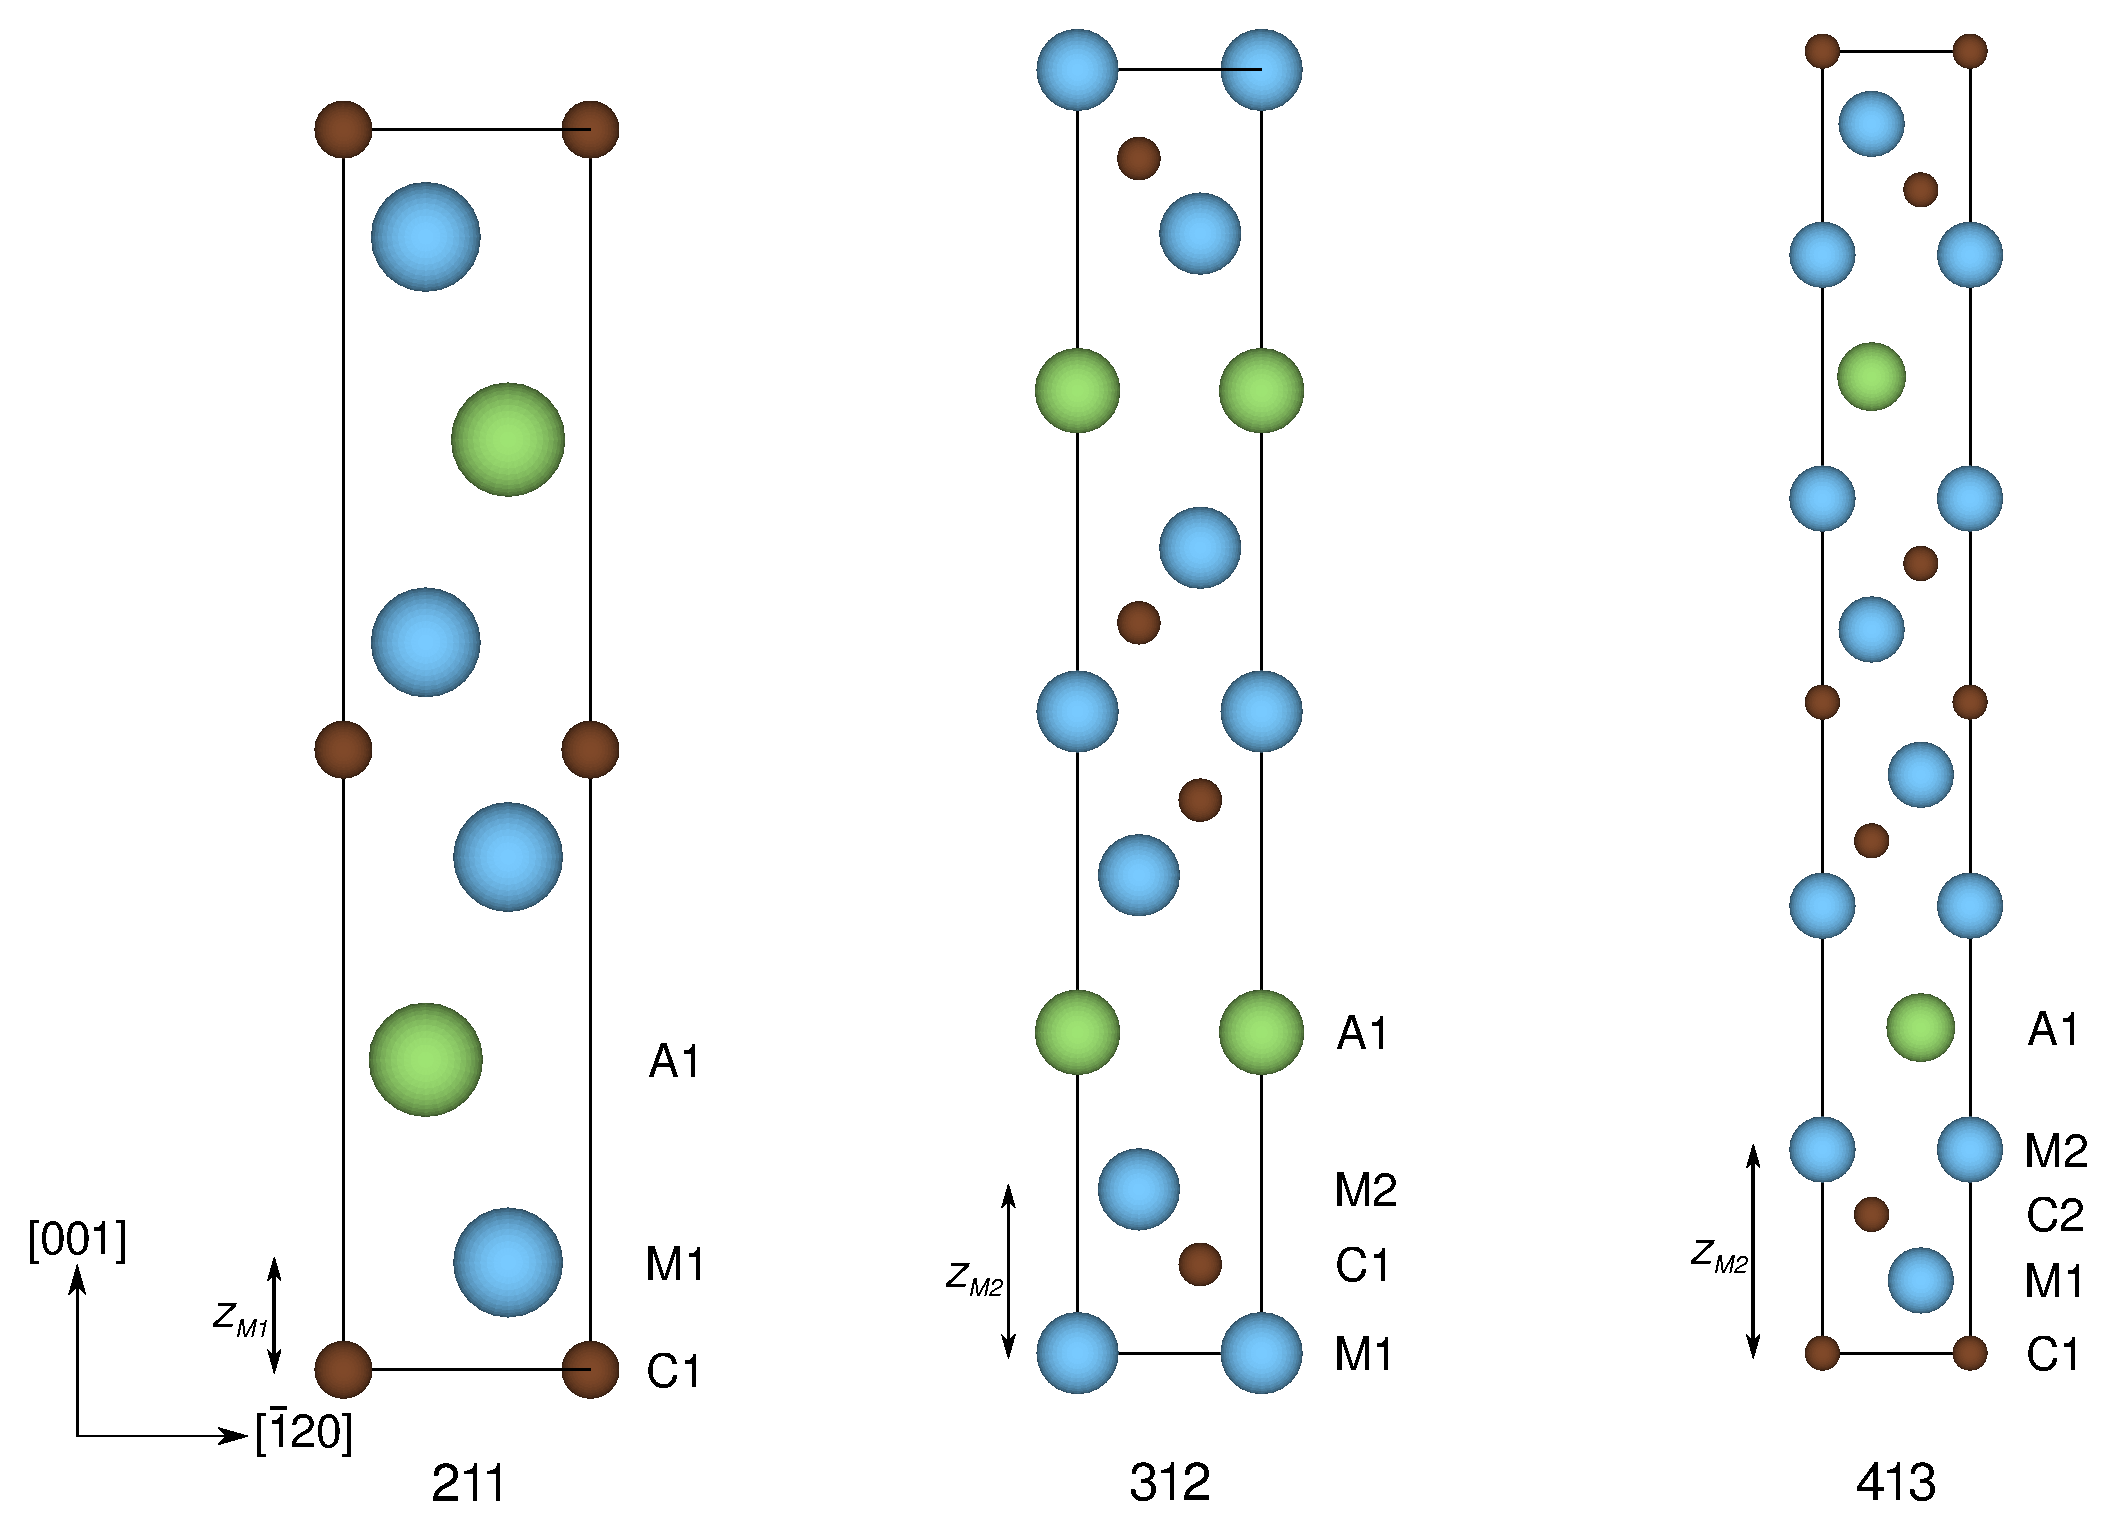
\includegraphics[width=\textwidth]{MAX_unit_cells}
\caption[The MAX phase unit cells.]{The unit cells of the first three possible MAX phases. Graphics prepared with VESTA \cite{Momma2011}.\label{fig:MAX_unit_cells}}
\end{figure}




\begin{figure}
\centering
\captionsetup{width=0.6\textwidth,font={sf,scriptsize},labelfont=bf}
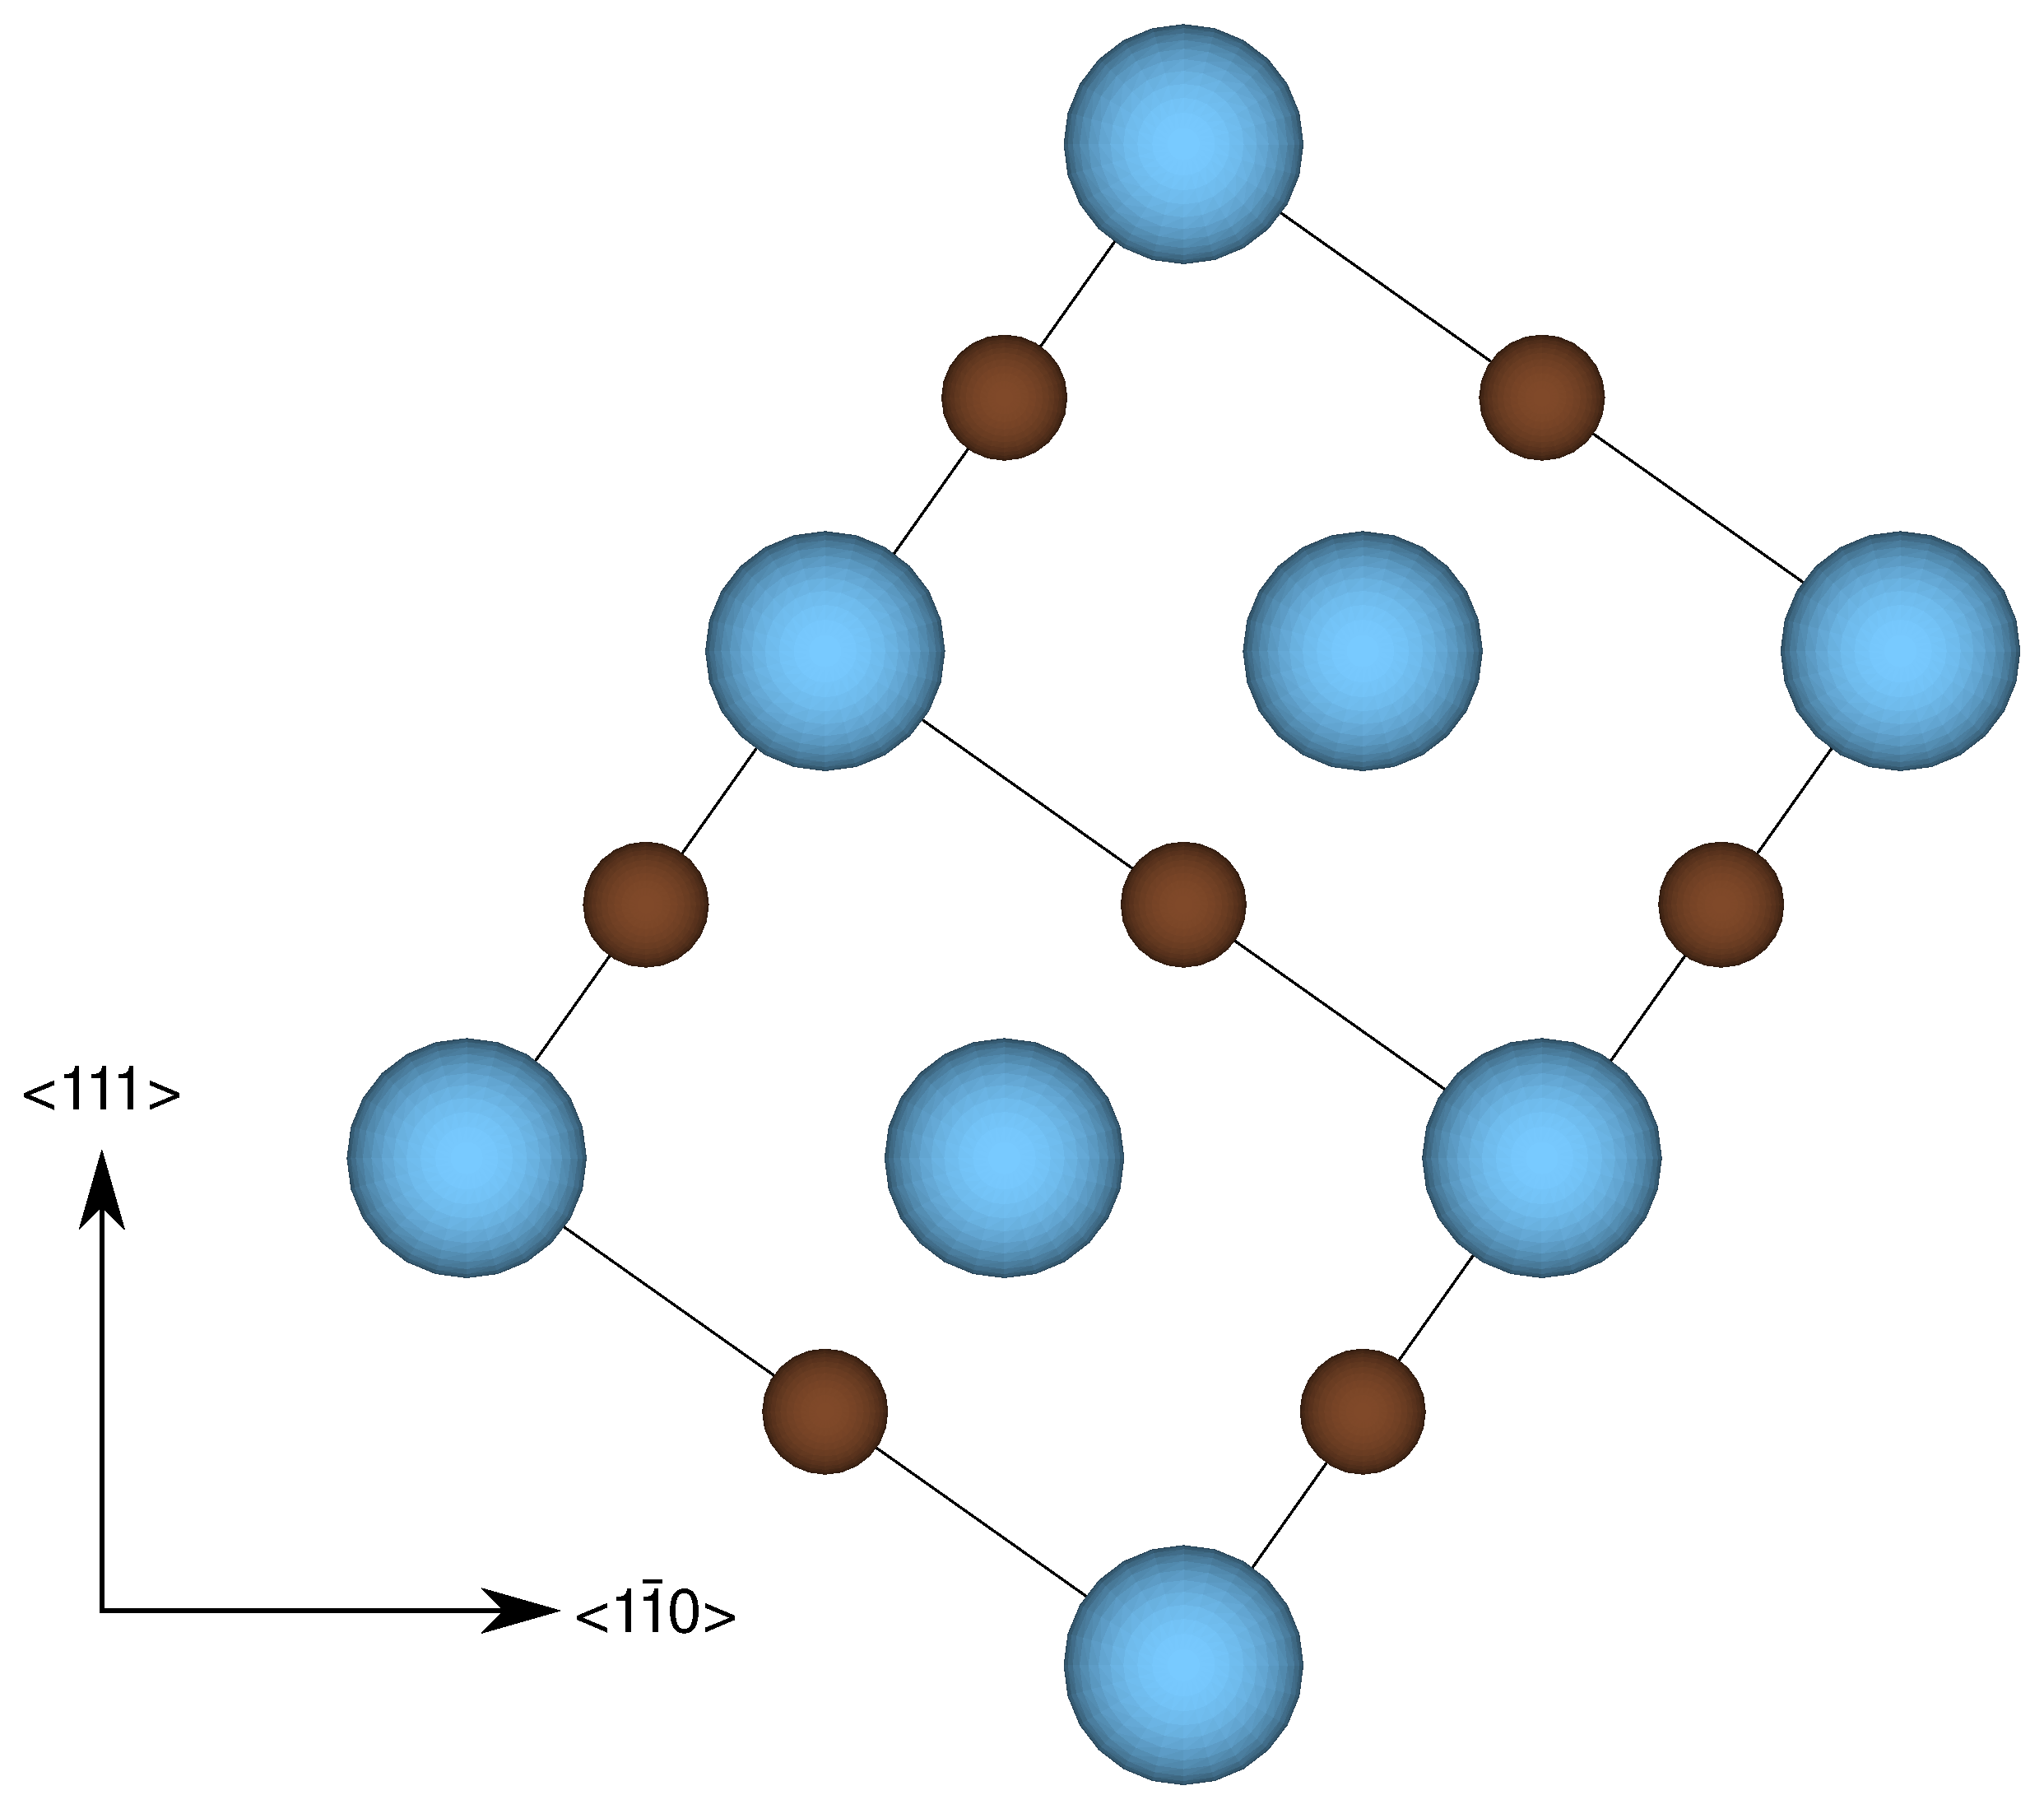
\includegraphics[width=0.5\textwidth]{TiC_111}
\caption[The unit cell of \ce{TiC}.]{The unit cell of \ce{TiC}, which has the rock salt structure, oriented to show the \{1\,1\,1\} planes which are equivalent to the MX layers of the MAX structure shown in \autoref{fig:MAX_unit_cells}. Graphic prepared with VESTA \cite{Momma2011}.\label{fig:TiC_111}}
\end{figure}


The description of complex crystals is often in terms of clusters of atoms that appear to pack together and fill space. The clusters may or may not have physical significance: for example clusters of up to 55 atoms of \ce{Ni}-\ce{Al} are stable on surfaces and so are clearly physically significant, but geometric descriptions of clusters can be made of simple materials like FCC aluminium \cite{Steurer2006}. Care must be taken therefore not to ascribe undue significance to purely geometric features, but the description of the MAX crystal structure as layers is not simply geometric but can be justified on the basis of heterogeneity in the chemical environments, i.e. the layers are meaningful.

The bonding in MAX phases has been shown, by density functional theory (DFT) calculations, to be a combination of metallic, covalent and ionic bonding but with covalent bonding predominant in the MX layer and metallic bonding in MA layers. Large variations in structural and mechanical properties are observed to depend on changes in the nature of this heterogeneous bonding character \cite{Radovic2013,Sun2011}. Notably the extreme (among MAX phases) properties of \ce{Ti2SC} are ascribed to the unusual strong bonding between \ce{Ti} and \ce{S} in addition to the strong bonding between \ce{Ti} and \ce{C} in contrast with most other MAX phases. This unusual bonding is taken to underlie the high elastic constants, $E =$~\SI{316}{\giga\pascal} the highest of any 211 MAX phase, and hardness of \SI{8}{\giga\pascal}, very nearly the highest of any bulk MAX phase \cite{Feng2010,Sun2011}.

\subsection{Deformation in MAX phases}

Deformation in \ce{Ti3SiC2} has been widely studied, particularly by Barsoum \cite{Farber1998,Barsoum1999,Farber1999,Barsoum1999dislocs_kinkbands,Barsoum2001}, and was found to readily occur by the glide of dislocations. Room temperature deformation was shown to increase the density of perfect basal dislocations with a Burgers vector equal to the lattice parameter $a$, so $b =$~<1\,1\,\={2}\,0>. 

Using heavily textured bulk samples of \ce{Ti3SiC2} the critical resolved shear stress of \ce{Ti3SiC2} was estimated by compression test. A sample with the basal planes of the sample oriented at approximately \SI{65}{\degree} to the compression axis and a yield stress of \SI{200}{\mega\pascal} was measured. Schmid's law is 

\begin{equation}
\tau_y = \sigma_y \cos{\phi} \cos{\lambda}
\end{equation}

where $\tau_y$ is the shear yield stress on the slip plane in question, $\sigma_y$ is the uniaxial yield stress\ $\phi$ is the angle between the slip plane normal and the loading axis, and $\lambda$ is the angle between the slip direction and the loading axis. The $\phi$ must be \SI{25}{\degree} ($=\SI{90}{\degree} - \SI{65}{\degree}$) but $\lambda$ is not known but if taken to be the maximum possible value, given $\phi=\SI{25}{\degree}$, of \SI{115}{\degree} then $\tau_y = \SI{77}{\mega\pascal}$, providing an upper bound \cite{Humphrey2012}. While this is higher than the estimate made by the original authors \cite{Barsoum1999}, \citet{Humphrey2012} points out that this is likely an overestimate due to the variation in Schmid factor across the sample and load redistribution between soft and hard grains but in any case is very low for a ceramic and approaches the flow stresses of pure cubic close-packed metals.


%%%%%%%%%%%%%%%%%%%%%%%%%%%%%%%%%%%%%%%%%%%%%%%%%%%%%%%%%%%%%%%%%%
%
%
%
%
%
%
% Figure about compression test here?
%
%
%
%
%
%
%%%%%%%%%%%%%%%%%%%%%%%%%%%%%%%%%%%%%%%%%%%%%%%%%%%%%%%%%%%%%%%


As discussed in \autoref{sec:tailor_peierls}, attempts have been made to explain and hence control the lattice resistance of materials, and this has been done for the MAX phases too. One study on MAX phases \cite{Music2007ductility} with the chemistry \ce{M2AlC} (M = Ti, V, Cr) used the more recent ductility criteria, namely Zhou-Carlsson-Thomson \cite{Zhou1994} and Rice \cite{Rice1992} which are discussed in detail in \autoref{sec:ductility_criteria}. There is recognition that the lattice resistance of a single dislocation, which is the limiting factor on ductility in most ceramics, is not simply dependent on bulk elastic constants. The authors therefore calculate ductility criteria based on stacking fault energies and surface energies, which necessitates choosing which plane to fault or cleave. In the MAX phases there are two natural choices: between the M atom and the A atom or between the M atom and the X atom. However there is no direct link, in these studies, between these properties and dislocation behaviour, and hence no direct link to the ductility. 

Some studies have considered the Peierls stress in complex crystals with layered structures \cite{Music2008,Emmerlich2009,Gouriet2015} but usually these have simply applied the result for an isotropic elastic material:
\begin{equation}
\tau_p = \frac{2G}{1-\nu} \exp \left( - \frac{2 \pi d}{b(1-\nu)} \right)
\end{equation}
where $G$ is the shear modulus, $\nu$ is the Poisson ratio, $d$ is the slip plane spacing and $b$ is the Burgers vector.


The result is therefore based on polycrystalline bulk elastic properties and the specifics of the MAX crystal structure are disregarded save the values of $d$ and $b$ chosen. These have tended to give high values of the Peierls stress, e.g. \SI{980}{\mega\pascal} for \ce{Ti2AlC} \cite{Music2008} which we can compare with \SI{700}{\mega\pascal} for \ce{TiC} \cite{Clegg2006}. The strength of \ce{TiC} should be an upper bound on the flow stress in the MAX phase, since the MAX phases contain planes of \ce{TiC}. Furthermore these planes of TiC in the MAX phases are equivalent to the slip planes in \ce{TiC} \cite{Hollox1966}. 

The GSF calculated by DFT has been used in at least one study \cite{Gouriet2015} but assumed that no change in confining elastic field occurred during dislocation motion, which has been shown to be significant \cite{Lubarda2007,Clegg2006}. \citet{Gouriet2015} also found Peierls stresses that are more similar to \ce{TiC}, of between \SI{611}{\mega\pascal} and \SI{957}{\mega\pascal}.

There is clearly a large effect of the crystal chemistry on the lattice resistance of the MAX phases which has not been adequately explained. If the effect can be understood it may allow a general route to tailoring the Peierls stress of a material and the introduction of a degree of ductility and toughness to otherwise brittle materials.



























































\section{Alternative energy formulations}

\label{sec:empirical_potentials}



The Peierls model is based on the assumption that energy changes can be largely approximated on elastic energy changes as a dislocation moves through a crystal lattice, but many materials do not fit this assumption well. While a full quantum-mechanical treatment of electronic structure by density functional theory calculations gives very accurate results for a very wide range of atoms and conditions the computational difficulty of describing all the valence electrons limits this to systems with hundreds or maybe a few thousands of atoms. Empirical potentials have been developed for a wide range of materials and conditions for the field of molecular dynamics and are more tractable computationally while hopefully retaining enough fidelity to elucidate the problem at hand \cite{martinez2013}.

Various potentials exist for different types of materials, usually according to the bonding present, for example the embedded atom method applies well to metals \cite{Daw1984}, the Lennard-Jones  and Buckingham potentials describe dispersion interactions and the short range exchange interaction arising from Pauli exclusion \cite{Jones1924,Buckingham1938} and bond order potentials describe covalent bonding, e.g. the Tersoff potential \cite{Tersoff1988}. 


Ionic solids are an obvious class of materials with which to demonstrate the application of alternative energy calculations by applying empirical potentials, although some modelling of dislocation motion by the conventional Peierls-Nabarro model, using the elastic properties and the generalised staking fault energy, have been undertaken for \ce{MgO} \cite{Miranda2005}, most ionic materials are not well represented by linear elasticity. 

There are large numbers of ionic solids with the same simple crystals structures, e.g. rocksalt, caesium chloride \cite{Kelly2012app7} and the primary contribution to the energy of these materials is the electrostatic interaction which is very simple:
\begin{equation}
U^{\text{electro}}_{ij} = \frac{1}{4\pi\epsilon_0} \frac{q_i q_j}{r_{ij}}
\end{equation}
where $\epsilon_0$ is the permittivity of free space, $q_i$ is the charge on atom $i$ and $r_{ij}$ is the separation between atoms $i$ and $j$.


The Lennard-Jones potential along with the electrostatic interaction is one of the simplest formulations to represent the interactions in ionic solids and has the form
\begin{equation}
\phi_{ij}(r_{ij}) = 4\epsilon_{ij} \left[ \left( \frac{\sigma_{ij}}{r_{ij}}\right)^{12}-     \left( \frac{\sigma_{ij}}{r_{ij}}\right)^6   \right]
\end{equation}
or in the ``A--B'' form
\begin{equation}
\phi_{ij}(r_{ij}) = \frac{A_{ij}}{r_{ij}^{12}} - \frac{B_{ij}}{r_{ij}^{6}}
\end{equation}
where $r_{ij}$ is the atomic separation, $\epsilon_{ij}$ is the depth of the energy minimum, $\sigma_{ij}$ is the (finite) atomic separation at which the energy is zero and $A_{ij}$ and $B_{ij}$ are simply parameters to be fitted and are related to $\epsilon_{ij}$ and $\sigma_{ij}$ by $A_{ij} = 4\epsilon_{ij}\sigma_{ij}^{12}$ and $B_{ij} = 4 \epsilon_{ij} \sigma_{ij}^{6}$. The total energy for a pair of atoms is then
\begin{equation}
U_{ij}(r_{ij}) = \frac{1}{4\pi\epsilon_0} \frac{q_i q_j}{r_{ij}} + \frac{A_{ij}}{r_{ij}^{12}} - \frac{B_{ij}}{r_{ij}^{6}}
\end{equation}




The energy of perfect ionic crystals is relatively easily calculated  via a Madelung or Ewald summation \cite{madelung1918,Ewald1921}, but usually these rely on an assumption of symmetry that is broken by the introduction of a defect. In the case of a dislocated crystal another approach is required. One option is a direct sum; the direct sum scales with the square of the number of atoms in the simulation, so if the distance from the dislocation line is considered the simulation time scales with the fourth power and can rapidly become intractable. However advances in computing power and efficient implementations of array operations in NumPy \cite{Numpy2011}, particularly an efficient implementation of the Einstein summation convention \cite{opt_einsum} may make this a workable solution.


An alternative is to use an implementation of a long range electrostatics solver that allows for non periodicity in two dimensions. One such implementation is the multiscale summation method in LAMMPS \cite{Hardy2009,LAMMPS_web}, which divides the problem into a short range potential and a series of smoothly vanishing long range potentials over increasingly coarse meshes at larger interatomic distances. The use of LAMMPS allows the inclusion of other energy terms such as polarisability of ions and so on.


\subsection{Dislocations in ionic crystals}
The rocksalt structure is particularly common in ionic solids and phases of this structure have been widely studied in terms of their plasticity. The slip direction is usually <110> and the active slip planes are \{001\} and \{1\={1}0\}, and sometimes \{1\={1}1\}. For edge dislocations the last would expose charged surfaces of atoms at free surfaces so despite being the closest packed plane it is not commonly seen \cite{Haasen1985}. Schematic illustrations of edge dislocations are shown in \autoref{fig:Schematic_NaCl_dislocs}.

\begin{figure}
\centering
    \begin{subfigure}{0.8\textwidth}
    \centering
    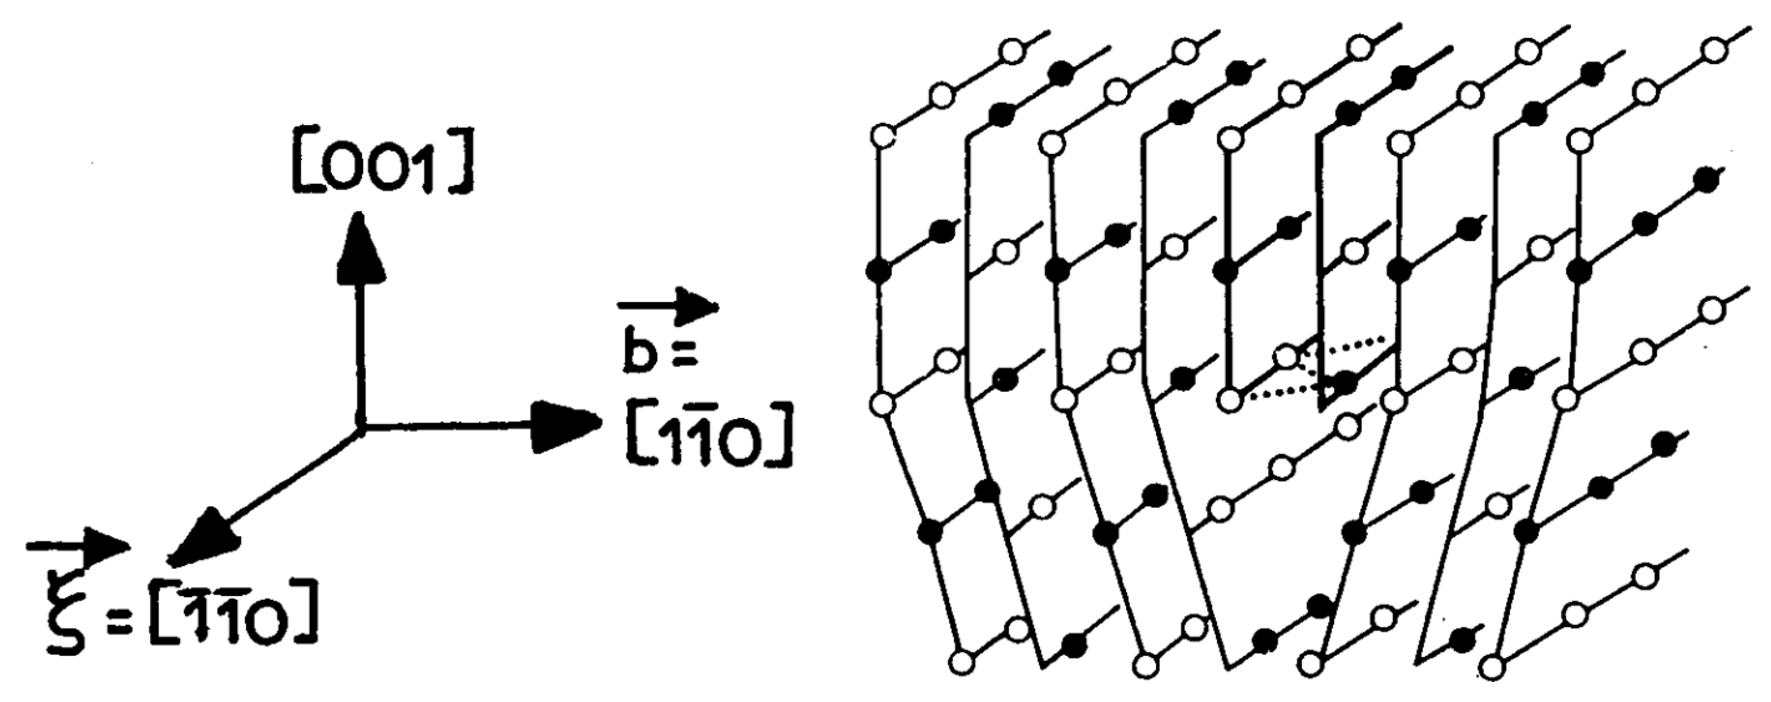
\includegraphics[width=\textwidth]{NaCl_001_1-10}
    \caption{The \{001\}<1\={1}0> slip system.}
    \end{subfigure}
\par\bigskip
    \begin{subfigure}{0.8\textwidth}
    \centering
    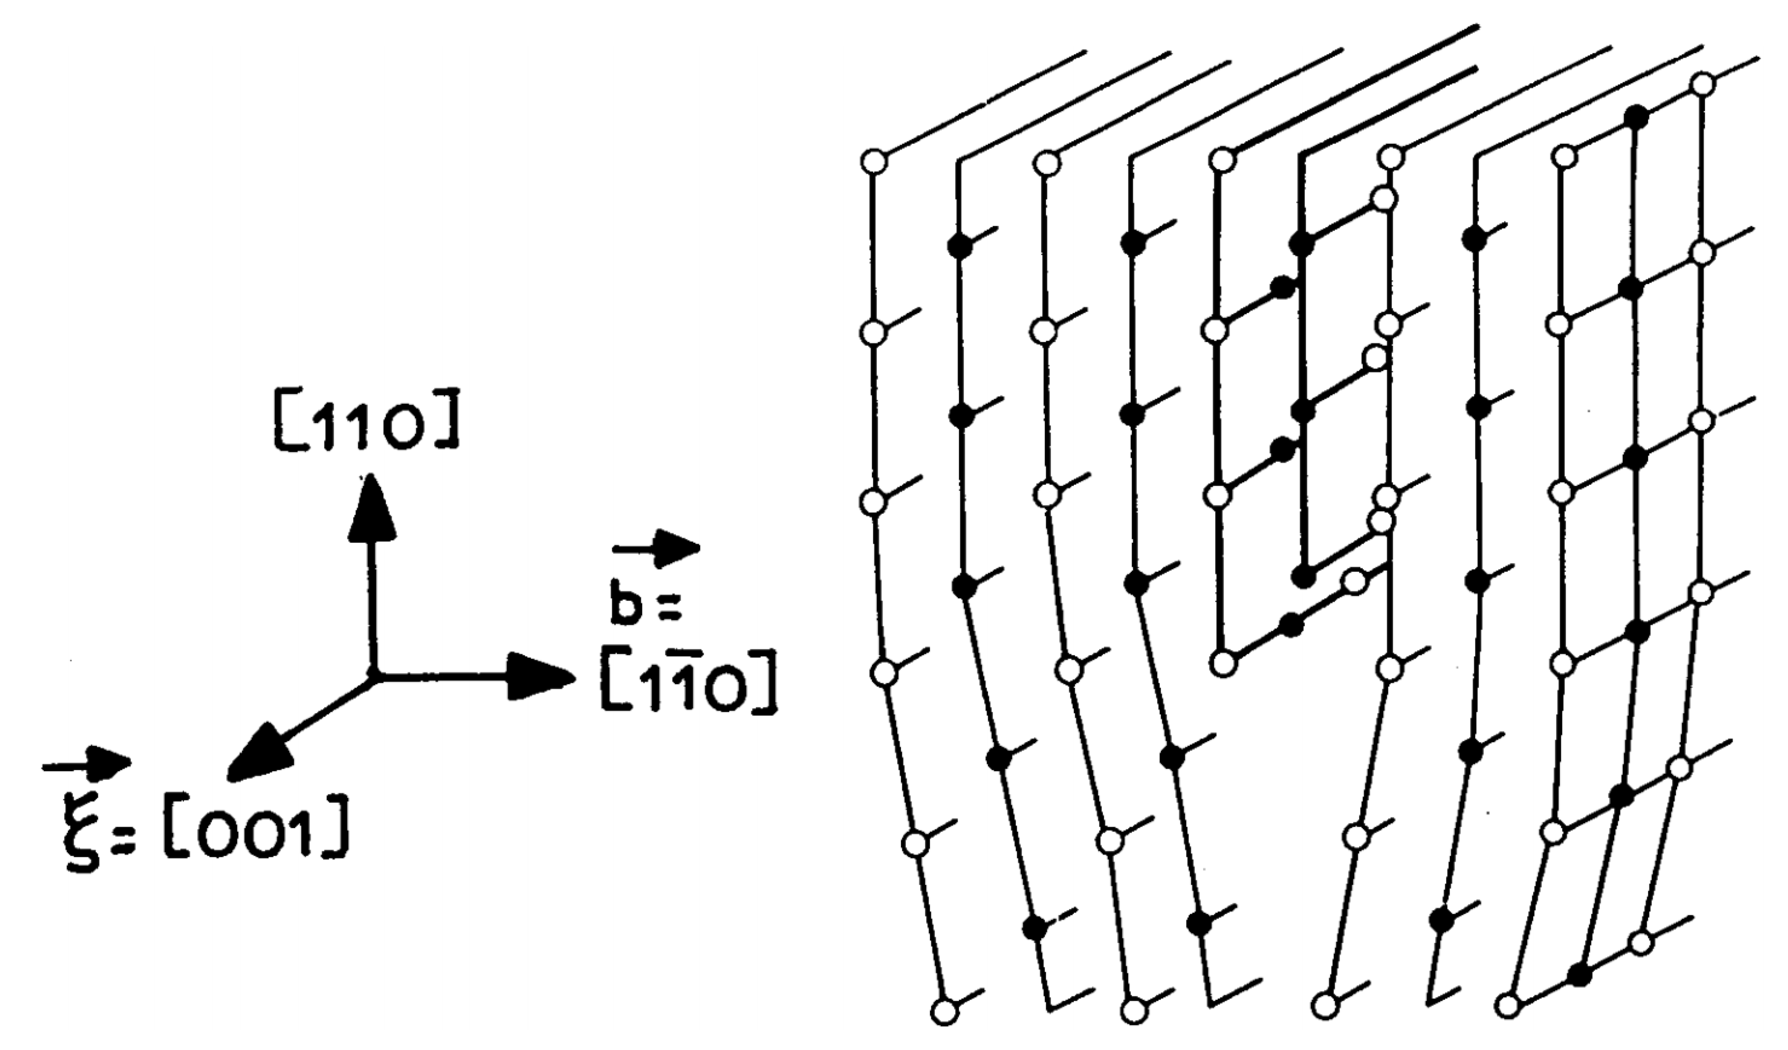
\includegraphics[width=\textwidth]{NaCl_110_1-10}
    \caption{The \{110\}<1\={1}0> slip system.}
    \end{subfigure}
\caption[Edge dislocations in the rock salt crystals.]{Schematic edge dislocations in the rocksalt structure reproduced from \cite{Haasen1985}. \label{fig:Schematic_NaCl_dislocs}}
\end{figure}





Experimental work has characterised flow stress of ionic solids with the rocksalt structure over a wide range of temperatures including very low temperatures using liquid helium (c.~\SI{4}{\kelvin}) and they deviate strongly from the prediction of elastic Peierls models. This makes them useful as a model system \cite{Haasen1985}.

Previous modelling of dislocations in ionic crystals has been undertaken, notably \citet{puls1976} who simulated edge \{001\}<1\={1}0> dislocations in \ce{MgO} and \citet{Woo1977} who modelled the same dislocation geometry in a range of ionic crystals with the rocksalt structure, among others \cite{Granzer1968,Woo1976,Hoagland1976,Brandt1987,Soullard1991,Foitzik1991}. These were limited by the computational resources available and used a variety of strategies to overcome these limits; one was to optimise only the equilibrium position and then assume linear trajectories for the atoms for intermediate states, as developed by \citet{Granzer1968}. This is similar to the assumption made by Peierls \cite{Peierls1940}, that the dislocation width does not vary between the equilibrium positions, which has been shown to have a very large effect on the results that are generated \cite{Clegg2006}.

Another method to overcome computational limitations was to simulate only small regions atomistically, applying a variety of boundary conditions, usually derived from elasticity both linear and non-linear in nature, to constrain the atomistic region and modelling material outside this core region as elastic, such conditions were used in \cite{Woo1977}. The use of conditions like these prevents the separation of the different energetic components since there is always a large contribution from the elastic region as well as the electrostatics and short-range interactions. A fully atomistic simulation would hopefully elucidate the energy contributions and aid insight into the dominant factors in controlling dislocation motion.

A fully atomistic model using suitable interatomic potentials will hopefully elucidate the factors that control dislocation motion in ionic solids.




























































































































\cleardoublepage
% the methods and results for building a new Peierls model
%*******************************************************************************
%****************************** Second Chapter *********************************
%*******************************************************************************

\chapter{A new Peierls model}
\label{chap:peierls_model}
\graphicspath{{peierls_model/Figs/}}

\epigraph{Complex is better than complicated}{\emph{The Zen of Python}}


Though there are a number \cite{Nabarro1947,Huntington1955, puls1976, Vitek1992,  Bulatov1997, Lubarda2007, Clegg2006,Gouriet2015} of Peierls models published in the literature over the decades since \citet{Peierls1940} first presented his solution, few have been applicable to situations beyond the initially envisaged problem, which is somewhat narrowly defined for an orthorhombic lattice that obeys linear elasticity. In this chapter a model is presented that allows  the consideration of energies defined by linear elasticity using the full elastic tensor, empirical potentials and generalised stacking fault energies. The model is also kept modular to allow extension to other formulations, e.g. a full quantum mechanical treatment using density functional theory.

The Python programming language was chosen for a number of reasons. Firstly the Python model is inherently modular, which provides a flexible structure, allowing parts of the model to be altered, extended or replaced quickly and easily. Secondly Python is also widely used for scientific computing, with a large body of documentation and a large support community. Finally Python has a very large number of extending modules providing advanced capabilities, particularly projects like NumPy and SciPy. NumPy provides a powerful and efficient implementation of arrays and a range of simple functions as well as more advanced linear algebra operations. SciPy is a project built on the basic data structure of the NumPy array and provides advanced algorithms and convenience functions including differential equations, numerical solvers and optimisers, image processing and statistical functions. The code written in this work has been published on-line \cite{code}. 

To calculate the Peierls stress we must find the changes in the dislocation energy as a dislocation moves from one low energy position to the next. The variable $\alpha$ is used to denote the  displacement of the dislocation as a fraction of the Burgers vector, $b$. Since boundary conditions are insufficient to define the atomic configuration, for each value of $\alpha$ the atomic configuration of the dislocation that minimises the energy must be found. Once sufficient samples of $\alpha$ have been made the Peierls stress can be calculated by 
\begin{equation}
\tau_p = \frac{1}{lb^2}   \left. \frac{\partial U}{\partial \alpha} \right|_{max} .
\end{equation}
where $l$ is the length of dislocation line for which the energy, $U$, is calculated for and $b$ is the Burgers vector.

For a given value of $\alpha$ the lowest energy configuration is found via three steps: first the definition, creation and representation of an atomic configuration, second the evaluation of the overall energy, and third the iterative improvement of the configuration to find the minimum energy. Taken together the first two steps can be thought of as a function that takes the value of $\alpha$ along with some input parameters as arguments and returns the total energy:

\begin{equation}
U_{\text{total}} = f(\alpha, p_1, p_2,...,p_n )
\label{eqn:energy_as_function}
\end{equation}
The input parameters, $p_i$, could be as general as the coordinates of every atom in the configuration or as specific as the single parameter defined by Peierls in his original treatment, the width of the dislocation. The main difference is trade off between computational tractability and the risk of over-constraining the model. Algorithms exist for finding the minimum of functions of the form given in \autoref{eqn:energy_as_function}. Such algorithms are much faster for functions with small numbers of parameters and some algorithms are not reliable for large numbers of parameters. Hence decisions about how to define an atomic configuration will have consequences for the optimisation of that configuration to find the lowest energy.

Here we use the positions of the atoms to define the configuration and then apply constraints to those rather than find the model limited by an assumption later. Hence individual atoms are represented in space by coordinates as an array of the form:
$$ atoms = \begin{pmatrix}
x_1 & y_1 & z_1  \\
x_2 & y_2 & z_2  \\
.   &.    &.     \\
.   &.    &.     \\
x_n & y_n & z_n  \\
\end{pmatrix}
$$
where $x_i$, $y_i$ and $z_i$ are coordinates in Euclidean space of the $i$th atom, in units of \r{A}ngstr\"{o}ms, i.e. \emph{not} relative to any crystallographic axes.

This representation can be extended: for example in the case of ionic solids the charge on each ion would be a necessary parameter for any energy calculation and would be represented thus:
$$
atoms = \begin{pmatrix}
x_1 & y_1 & z_1 & q_1 \\
x_2 & y_2 & z_2 & q_2 \\
.   &.    &.    &.    \\
.   &.    &.    &.    \\
x_n & y_n & z_n & q_n \\
\end{pmatrix}
$$

This could be extended to an arbitrary number of parameters such as parameters for empirical potentials, labels for symmetrically distinct ions of the same species etc.





\section{Building a dislocation}
\FloatBarrier
\label{sec:build}




The model might be expected to start in the same way as Peierls; bringing together two half crystals as shown in \autoref{fig:semi_infinite_crystals} and simply allowing the structure to relax, leaving all the atomic positions as free variables. However there are two reasons to apply constraints to the atomic coordinates: firstly constraints reduce the number of parameters to search and secondly an unconstrained global optimisation might remove the dislocation entirely. This would create a perfect crystal, which would have a lower energy than a dislocated crystal. To achieve this a displacement field based on initial atomic coordinates is used to find a final atomic configuration.

For a given value of $\alpha$, there will be an initial configuration of atoms defined by two half crystals brought together at a slip plane with some relative displacement between them defined by $\alpha$ and the Burgers vector. The core of the dislocation is taken to be the line where $x,y = 0$. The position of the core with respect to the lattice of the half crystals is defined by $\alpha$, usually with $\alpha=0$ defining the configuration in which the extra half-plane of atoms aligns with the dislocation core, as shown in \autoref{fig:joined_half_crystals}. 

The final, in the sense of ready to be evaluated energetically rather than optimised, configuration is the combination of  the initial positions and an array of displacements defined by some displacement field, $\bm{\delta}(x_0, y_0, z_0)$, i.e.
\begin{equation}
\mathbf{r}_i = \mathbf{r}_i^0 + \bm{\delta}(\bm{r}_i^0)
\end{equation}
where $\mathbf{r}_i$ is the position vector defining the final position of the $i$th atom, $\mathbf{r}_i^0$ is the vector defining the initial position of the $i$th ion and $\bm{\delta}$ is a vector displacement field.


%%%%%%%%%%%%%%%%%%%%%%%%%%%%%%%%%%%%%%%%%%%%%%%%%%%%%%%%%%%%%%%%%%%%%%%%%%%5
%
%                      Initial half crystals
%
%%%%%%%%%%%%%%%%%%%%%%%%%%%%%%%%%%%%%%%%%%%%%%%%%%%%%%%%%%%%%%%%%%%%%%%%%%%%%%
\subsection{Defining the initial atomic positions}


Firstly we must define the initial positions of the atoms in the half crystals. In the Peierls model the material was assumed to be a simple orthorhombic lattice; i.e. a misaligned  bond across the slip plane has a minimum energy when the bond is normal to the slip plane. To consider the effects of the particular structure the atomic configuration must be generated from the lattice and motif of the perfect crystal.

To create a crystal conveniently oriented with respect to the Cartesian reference axes and the crystal slip system, unconventional unit cells were defined. Directions and planes defined relative to the unconventional or dislocation cell will be marked prime, e.g. $[1\,0\,0]'$. The Burgers vector $\mathbf{b}$ is taken to be the $[1\,0\,0]'$, the shortest slip plane normal that is a full lattice vector is taken to be $[0\,1\,0]'$ and the $[0\,0\,1]'$, parallel to the line vector, is the shortest lattice vector that is perpendicular to both the Burgers vector and the slip plane normal and its sign is such that the axes are right handed. Filling space by combining a motif and a lattice defined according to these axes is convenient because most of the mathematical results of dislocation theory, stress and strains fields etc., are defined taking $x$, $y$ and $z$ parallel to $[1\,0\,0]'$, $[0\,1\,0]'$, $[0\,0\,1]'$ respectively.

For example the \ce{NaCl} <1\,\={1}\,0>\{1\,1\,0\} slip system gives a new unit cell aligned with the slip system:

\begin{equation*}
\begin{aligned}[c]
{[1\,0\,0]}' &=\, ^{1}\!/_{2} [1\,1\,0]   \\
{[0\,1\,0]}' &=\, ^{1}\!/_{2} [1\,\overline{1}\,0]   \\
{[0\,0\,1]}' &=\, [0\,0\,1]   
\end{aligned}[c]
\qquad
\begin{aligned}[c]
&\parallel \mathbf{b} \\
&\parallel \mathbf{d} \\
&\parallel \mathbf{l}
\end{aligned}
\end{equation*}
where $\mathbf{l}$ is the line vector of the dislocation.


The atoms in this non-conventional unit cell are
$$
motif = \begin{pmatrix}
0 & 0 & 0 & +1 \\
^{1}\!/_{2} & ^{1}\!/_{2} & ^{1}\!/_{2} & +1 \\
0 & 0 & ^{1}\!/_{2} & -1 \\
^{1}\!/_{2} & ^{1}\!/_{2} & 0 & -1 \\
\end{pmatrix}
$$
where a $+1$ in the final column denotes the positive charge of a sodium ion and a $-1$ denotes the negative charge of a chloride ion.



\begin{figure}
\centering


    \begin{subfigure}{0.55\textwidth}
    \centering
    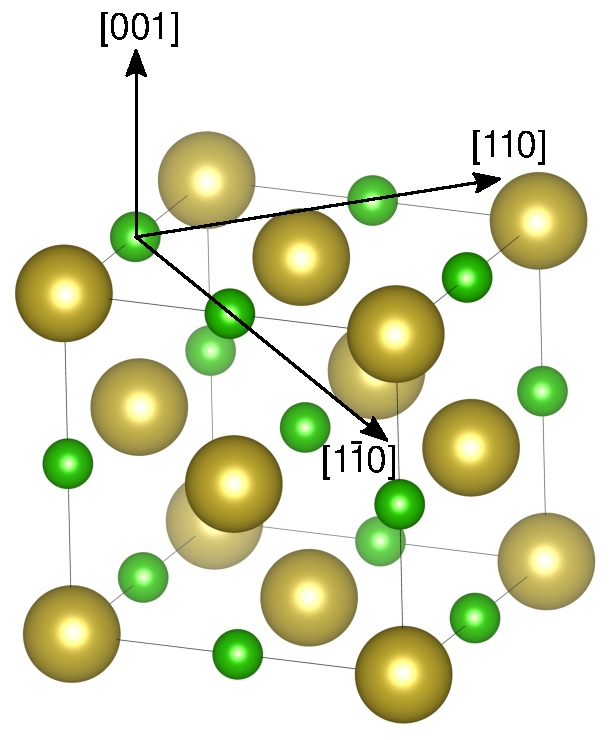
\includegraphics[width=\textwidth]{NaCl_conventional_unit_cell}
    \caption{The conventional unit cell of sodium chloride with the salient slip directions and plane normals highlighted. \label{fig:NaCl_conventional_cell_slip_system_marked}}
    \end{subfigure}

    \begin{subfigure}{0.4\textwidth}
    \centering
    \includegraphics[height=2.0in]{NaCl_110_110}
    \caption{The sodium chloride unit cell best aligned with the <1\,1\,0>\{1\,\={1}\,0\} slip system. \label{fig:NaCl_110_110_unit_cell}}
    \end{subfigure}
    ~
    \begin{subfigure}{0.4\textwidth}
    \centering
    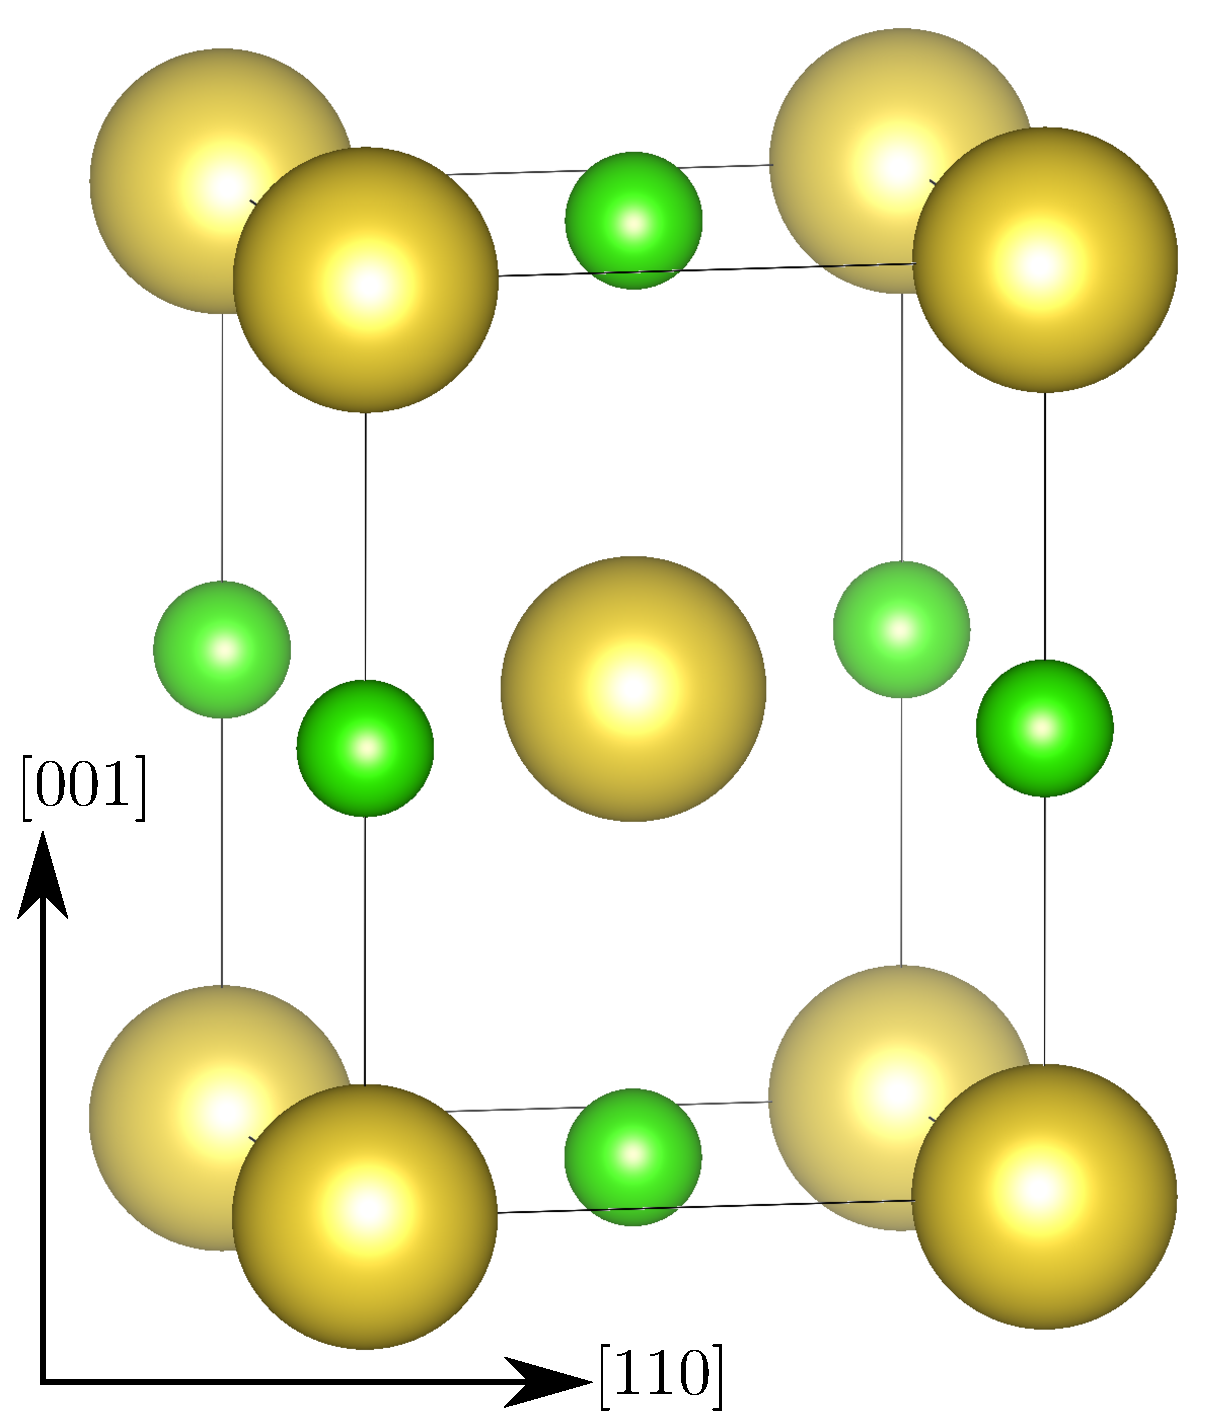
\includegraphics[height=2.5in]{NaCl_110_001}
    \caption{The sodium chloride unit cell best aligned with the <1\,1\,0>\{0\,0\,1\} slip system. \label{fig:NaCl_110_001_unit_cell}}
    \end{subfigure}

\caption[Unconventional unit cells of rock salt to build a dislocation.]{Possible unit cells for sodium chloride showing the conventional unit cell and two unconventional unit cells with the new crystallographic axes aligned to slip system, i.e. the Burgers vector and slip plane normal. Graphics prepared with VESTA \cite{Momma2011}.\label{fig:unconventional_NaCl_unit_cells}}
\end{figure}






Similarly the \ce{NaCl} <1\,\={1}\,0>\{0\,0\,1\} slip system is defined by the unit cell:
\begin{equation*}
\begin{aligned}[c]
 {[1\,0\,0]}' &=\, ^{1}\!/_{2} [1\,1\,0] \\
 {[0\,1\,0]}' &=\,  [0\,0\,1] \\
 {[0\,0\,1]}' &=\; ^{1}\!/_{2} [1\,\overline{1}\,0] \\
\end{aligned}
\qquad
\begin{aligned}[c]
&\parallel \mathbf{b} \\
&\parallel \mathbf{d} \\
&\parallel \mathbf{l}
\end{aligned}
\end{equation*}
and the atoms are
$$
motif = \begin{pmatrix}
0 & 0 & 0 & +1 \\
^{1}\!/_{2} & ^{1}\!/_{2} & ^{1}\!/_{2} & +1 \\
^{1}\!/_{2} & 0 & ^{1}\!/_{2} & -1 \\
0 & ^{1}\!/_{2} & 0 & -1
\end{pmatrix}
$$


These unit cells are shown in relation to the conventional cell in \autoref{fig:unconventional_NaCl_unit_cells}. With these unit cells we can convolve the motif with a lattice to generate an initially perfect crystal defined with respect to Cartesian axes aligned with the slip system. Two offsets are then applied; firstly the half crystal below the slip plane, which is defined by $y < 0$, will be offset in the positive $x$ direction by $b/2$ and then the entire crystal is offset to put the dislocation core in the desired location. The latter will require an offset along the slip direction, $[0\,0\,1]'$ of $\alpha b$ and an additional offset in the $[0\,1\,0]'$ direction. While the magnitude of this offset is not necessarily predictable, in the case of \ce{NaCl} the core must be at a height of $d/4$ in order to be halfway between the two (0\,2\,0) layers.

The initial positions of the atoms in the dislocated crystal are related to those of an initially perfect crystal by
\begin{equation}
\bm{r_i^0} = \bm{r_i^{\text{perfect}}} +\begin{cases}
[-\alpha{}b, h, 0] & \quad \text{if } y_i^{\text{perfect}} > 0\\
[b(1/2 - \alpha{}), h, 0] & \quad \text{if } y_i^{\text{perfect}} < 0\\
\end{cases} 
\end{equation}

The offset to the atomic coordinates in $-\alpha{}b$ such that as $\alpha$ increases the dislocation motion is in the positive $x$ direction.





\FloatBarrier












%%%%%%%%%%%%%%%%%%%%%%%%%%%%%%%%%%%%%%%%%%%%%%%%%%%%%%%%%%%%%%%%%%%%%%%%%%%%%%%%%%%

                          % Displacement fields

\subsection{Displacement fields}

A suitable displacement field is required. First we can take a Volterra dislocation, which in a continuous isotropic elastic medium has a displacement field \cite{Hirth1982Straight_dislocs}:
\begin{subequations}
\begin{align}
u &= \frac{b}{2\pi}\left[ \arctan\left(\frac{x}{y}\right) + \frac{xy}{2(1-\nu)(x^2 + y^2)} \right] \\[0.5ex]
v &= -\frac{b}{2\pi} \left[ \frac{1-2\nu}{4(1-\nu)} \ln(x^2 + y^2) + \frac{x^2 + y^2}{4(1-\nu)(x^2 + y^2)} \right]
\end{align}
\end{subequations}
where $u$ and $v$ are the components of the displacement field parallel to $x$ and $y$ respectively, $x$ is the initial position parallel to the Burgers vector, $y$ is the initial position parallel to the slip plane normal, $b$ is the magnitude of the Burgers vector and $\nu$ is the Poisson ratio of the material. The terms all converge to fixed values at large $x$ or $y$ except the logarithmic component of $v$. This represents the bending of a single crystal that arises from the introduction of an extra half plane \cite{Hirth1982Straight_dislocs}.

This formulation of the displacement field and subsequent solution for an isotropic elastic continuum is discontinuous, diverging at $r=0$, where $r=\sqrt[]{x^2+y^2}$. To remove the discontinuity \citet{Eshelby1949} proposed considering a single dislocation to be composed of a continuous distribution of dislocations with infinitesimal Burgers vectors, the integral of which yields the Burgers vector of the full dislocation. 

By considering the local strains (a normal strain parallel to the slip plane) due to this distribution, the stress on the slip plane can be found. By applying a force balance condition with the stress arising due to the misalignments, the displacements at the slip plane can be found, following the arguments laid out in \cite{Hirth_Lothe1982lattice_periodicity}. 

Let $\mathbf{b}'dx'$ be the Burgers vector of an infinitesimal dislocation lying between $x'$ and $x'+dx'$. The dislocation corresponds to a displacement of $-2(du/dx)dx'$. The total Burgers vector can be found by integration:
\begin{equation}
b = \int_{-\infty}^{\infty} b'(x') \dd x' = -2\int^{\infty}_{-\infty} \left( \! \frac{\dd u}{\dd x} \right)_{x=x'} \dd x' 
\end{equation}

The shear stress due to a Volterra dislocation  is \cite{hirth_lothe1982peierls_displacements}
\begin{equation}
\sigma^{\text{Volterra}}_{xy} = \frac{\mu b}{2\pi (1-\nu)} \frac{x(x^2 - y^2)}{(x^2+y^2)^2}
\end{equation}
where $x$ relates to the the core of the single dislocation, centred on the origin, with Burgers vector $b$.

The shear stress on the slip plane due to a single Volterra dislocation is found, by setting $y=0$ and substituting for $b$, to be
\begin{equation}
\sigma^{\text{Volterra}}_{xy}(x,0) = -\frac{\mu}{2\pi(1-\nu)} \int^{\infty}_{-\infty} \frac{b'}{x-x'} \!\dd x' =  \frac{\mu}{\pi(1-\nu)} \int^{\infty}_{-\infty} \frac{1}{x-x'} \left(\!\frac{\dd u}{\dd x}\right)_{x=x'} \!\dd x'
\label{eqn:elastic_stress_at_slip_plane}
\end{equation}
where $x-x'$ is the distance between some point $x$ and the infinitesimal dislocation at $x'$.

At the minimum energy position the net stress on the slip plane, i.e all $(x,0)$, vanishes, so there must be a balancing stress arising from the misalignment of the material across the slip plane. By analogy with \citet{Frenkel1926}:
\begin{equation}
\sigma_{xy}^{\text{misalignment}}(x,0) = C \sin \left( \frac{2\pi \phi}{b} \right)
\end{equation}
or in terms of the displacements either side of the slip plane:
\begin{equation}
\sigma_{xy}^{\text{misalignment}}(x,0) = -C \sin \left( \frac{4\pi u}{b} \right)
\end{equation}
If Hooke's law is satisfied at small strains we can write
\begin{equation}
\sigma_{xy}^{\text{misalignment}}(x,0) = 2 \mu \varepsilon_{xy} = \frac{\mu{}\phi}{d}
\label{eqn:misalign_stress_at_slip_plane}
\end{equation}
We can combine \autoref{eqn:elastic_stress_at_slip_plane} and \autoref{eqn:misalign_stress_at_slip_plane} to give an integral equation thus:
\begin{equation}
\int^{\infty}_{-\infty} \frac{1}{x-x'} \left(\!\frac{\dd u}{\dd x}\right)_{x=x'} \dd x' = \frac{b(1-\nu)}{2d} \sin\left(\frac{4\pi{}u}{b}\right)
\end{equation}
A solution is \cite{hirth_lothe1982peierls_displacements, Eshelby1949}
\begin{equation}
u(x) = -\frac{b}{2\pi} \arctan \left( \frac{x}{w} \right)
\label{eqn:one_dimensional_displacements}
\end{equation}
where $w$ is the half width of the dislocation and, for an isotropic elastic solid, has the value
\begin{equation}
w = \frac{d}{2(1-\nu)}.\label{eqn:half_width}
\end{equation}
\autoref{eqn:one_dimensional_displacements} satisfies the boundary condition that $u(\infty) = - u(-\infty) = -b/4$. $x=w$ gives $u(w)=1/2\, u(\infty)$, i.e. in the region $-w < x < w$ the disregistry across the slip plane is greater than half the maximum that occurs at $x=0$.

The two dimensional case gives a displacement field \cite{Eshelby1949,Leibfried1949,nabarro1987theory}:
\begin{subequations}\label{eqn:displacements}
\begin{align}
u(x,y) &= \frac{b}{2\pi} \left( \arctan \left[ \frac{y +  w\frac{|y|}{y}}{x} \right] - \frac{\pi}{2} \frac{|y|}{y} \frac{|x|}{x} \right) + c_1 \frac{xy}{x^{2} + (y + w\frac{|y|}{y} )^2} \\
v^y(x,y) &= c_2 \frac{y(y +  w \frac{|y|}{y})}{x^2 + (y +  w \frac{|y|}{y})^2} + c_3 \ln \left| \frac{x^2 + (y +  w \frac{|y|}{y})^2}{b^2} \right|
\end{align}
\label{eqn:displacement_field}
\end{subequations}
The final atomic configuration is then defined by 
\begin{equation}
\bm{r}_i = \bm{r}_i^0 + [u_i\,\bm{\mathrm{\hat{i}}},\; v_i\,\bm{\mathrm{\hat{j}}},\; 0\,\bm{\mathrm{\hat{k}}}]
\end{equation}

These terms can be interpreted physically: the arctan term is the same as in the original Peierls treatment, representing displacements along the slip plane that alter the local misalignment across the slip plane. The terms with the prefactors $c_1$ and $c_2$ represent shear strains: the $xy$ and $yx$ shears respectively. The logarithmic term, with the prefactor $c_3$, represents the bending of the entire crystal that must arise from the introduction of an extra half plane of atoms. This logarithmic term does not converge to a constant value at large $x$ or $y$, but this is consistent with this physical interpretation \cite{hirth_lothe1982peierls_displacements}.

Hence the parameters have physical interpretations: The width of the dislocation still defines the region with large disregistries, while $c_1$ and $c_2$ define the magnitude of displacements associated with shear strains around the dislocation core and $c_3$ defines the magnitude of the bending of a crystal that must arise from the introduction of an extra half plane of atoms.
To illustrate the displacements produced by these different terms some exaggerated (by a factor of ten from that predicted for an isotropic elastic medium) dislocation configurations are shown in \autoref{fig:parameters_of_the_disloc_configuration}.




\begin{figure}
\centering

    \begin{subfigure}{0.4\textwidth}
    \centering
    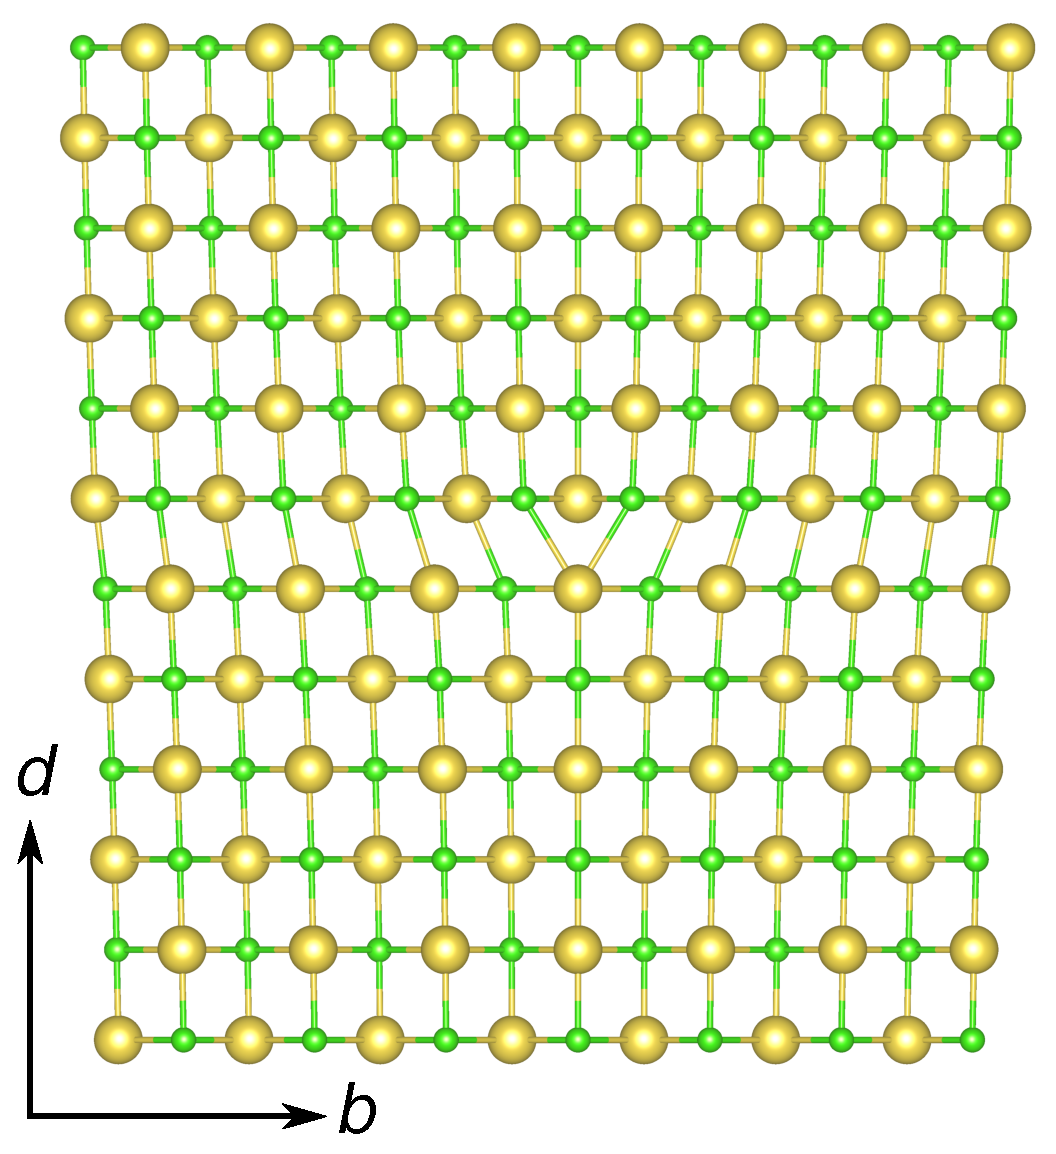
\includegraphics[width=0.6\textwidth]{wide_NaCl}
    \caption{A dislocation with a large width.}
    \end{subfigure}
    ~
    \begin{subfigure}{0.4\textwidth}
    \centering
    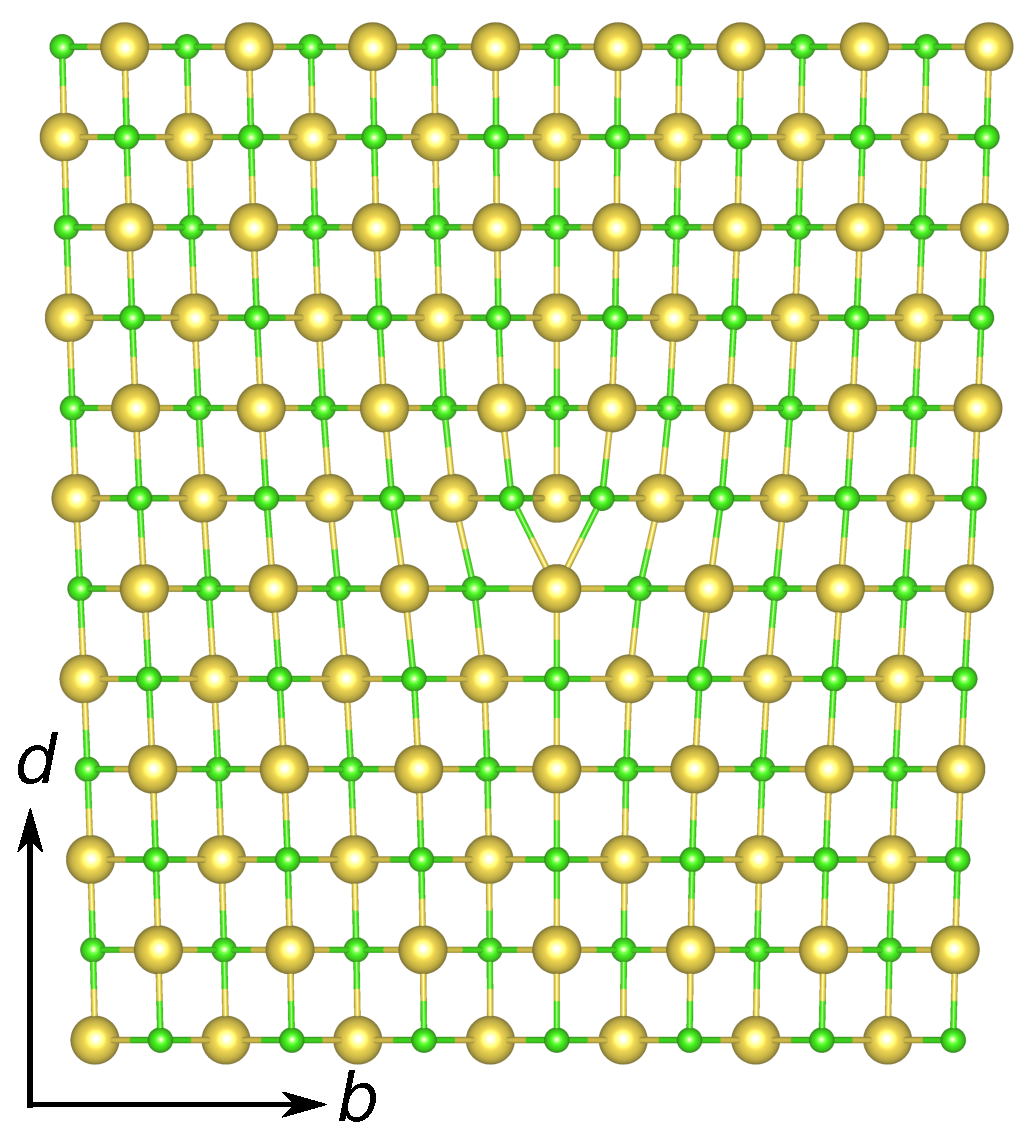
\includegraphics[width=0.6\textwidth]{narrow_NaCl}
    \caption{A dislocation with a small width.}
    \end{subfigure}

	\begin{subfigure}{0.4\textwidth}
	\centering
    \includegraphics[width=0.6\textwidth]{large_c1_NaCl}
    \caption{Large values of $c_1$ and $c_2$.}
	\end{subfigure}
    ~
	\begin{subfigure}{0.4\textwidth}
	\centering
    \includegraphics[width=0.6\textwidth]{large_c3_NaCl}
    \caption{A large value of $c_3$.}
	\end{subfigure}

    \begin{subfigure}{0.8\textwidth}
    \centering
    \includegraphics[width=0.5\textwidth]{typical_NaCl}
    \caption{A ``typical'' configuration.}
    \end{subfigure}

\captionsetup{width=0.8\textwidth}
\caption[The displacement field around an edge dislocation in rock salt.]{Various configurations of sodium chloride <1\,1\,0>\{0\,0\,1\} dislocations demonstrating the effects of the parameters of the displacement field defined in \autoref{eqn:displacements}, $w$, $c_1$, $c_2$ and $c_3$. Typical parameters are taken to be those predicted for an isotropic elastic material as given in  Equations~\ref{eqn:half_width} and \ref{eqn:disloc_params}, giving \SI{1.78}{\angstrom}, \SI{0.40}{\angstrom}, \SI{0.40}{\angstrom} and \SI{-0.12}{\angstrom} respectively for sodium chloride. Exaggerated values were ten times that. Calculated with $\nu =$~\num{0.207} and $a =$~\SI{5.644}{\angstrom} \cite{Theocaris1994,Rao1990}. Graphics prepared with VESTA \cite{Momma2011}.\label{fig:parameters_of_the_disloc_configuration}}
\end{figure}


The inclusion of $v(x,y)$ in the displacement field means that there will always be some finite displacement normal to the slip plane. This is expected and is be associated with phenomena such as pressure dependent yield stress \cite{frost1982pressure}. These displacements might also be responsible for the normal strains observed around line defects in layered crystals that have been ascribed to  a new class of defect called ripplocations \cite{Gruber2016}.




For an isotropic elastic medium the various parameters in \autoref{eqn:displacement_field} are found analytically  to have fixed values for the lowest energy dislocation. The half-width, $w$, takes the same value as in \autoref{eqn:half_width} and the three other parameters are defined by
\begin{subequations}\label{eqn:disloc_params}
\begin{align}
c_1 &= \frac{b}{4\pi{}(1-\nu)} \\
c_2 &= \frac{b}{4\pi{}(1-\nu)} \\
c_3 &= - \frac{b(1-2\nu)}{8\pi(1-\nu)}.
\end{align}
\label{eqn:expressions_for_the_ideal_disloca_parameters}
\end{subequations}
The terms of the form $|x|/x$ and $|y|/y$ are to give all the terms the right sense in the right regions of space, i.e. above and below the slip plane in $y$ and either side of the dislocation in $x$. This reduces to the simpler solution in \autoref{eqn:one_dimensional_displacements} if only the atoms adjacent to the slip plane are considered. This form is useful because it is continuous and finite for all values of $x$ and $y$. 


This gives a displacement field for a general material  which has four parameters: the width, $w$, and the scaling factors, $c_1$, $c_2$ and $c_3$. These parameters are varied to find the lowest energy dislocation. If the energy is calculated by an atomistic model, rather than by continuum elasticity, then there is no analytical solution for these parameters. Instead those values that minimise the energy are taken to be the correct solution.







A final note on the parametrisation of the dislocation structure is that the values $c_1$, $c_2$ and $c_3$ are not constrained. The purely isotropic case described above the parameters $c_1$, $c_2$ are positive and $c_3$ is negative, but there is no physical reason they cannot have a different sign. However a negative value of the width is not physically meaningful in this formulation. A negative width reintroduces the discontinuity at which displacements would diverge (in fact it would introduce two, one either side of the slip plane). Hence the constraint that $w>0$ is applied, but $c_1$, $c_2$ and $c_3$ are allowed to vary freely.





































\section{Evaluating the dislocation energy}
\label{sec:dislocation_energy}



Since there are insufficient boundary conditions to completely define a dislocation configuration with even four parameters the energy of the dislocation is the only way to identify a``correct'' or true configuration. Hence we must characterise the energy of arbitrary configurations. One obvious method to calculate the energy is to try and replicate the model based on elastic energy in the two half crystals and misalignment energy across the slip plane, there is the opportunity to calculate the full strain tensor and along with single crystal elastic constants the effects of elastic anisotropy can be taken into account. Another would be to use empirical potentials similar to those used in molecular dynamics; this would allow the exploration of dislocation properties in materials that are not well modelled by elasticity, ionic solids or compound semiconductors are examples of materials where elasticity is probably less appropriate. Both of these approaches are explored.

\subsection{Strain energy and misalignment energy}

This approach builds on the original approach of \citet{Peierls1940} and then \citet{Nabarro1947} and explains how the dislocation is stable due to a balancing of two forces, there is a force that attempts to spread the dislocation out into a planar defect, this arises due to the elastic stored energy in the bonds either side of the slip plane which would be zero in the case of a planar defect, which can be described by an infinitely wide dislocation. The other force tends to narrow the dislocation, this arises due to the misfit or misalignment across the slip plane. This would be a maximum for the planar defect where the entire slip plane is misaligned and would decrease monotonically as the width decreases.

Using this approach to the energy has a number of advantages. A two dimensional model is sufficient since for a long dislocation the condition of plane strain can be applied. If elastic theory can be applied at the scale of the unit cell then displacements need only be considered between unit cells rather than within them, which simplifies the model considerably.

\subsection{Strain energy}

Firstly the elastic energy can be easily calculated for a small volume if the strain and the elastic tensor is known. A good discussion of tensors and elasticity is given by \citet{kelly_knowles2012chapter5_tensors,kelly_knowles2012chapter6_stress_strain} and a discussion of elasticity in the context of dislocation theory is given by \citet{hirth_lothe1982elasticity}. The salient results are drawn together here.

Hookes law can be written as a tensor relationship using the einstein summation convention:
\begin{equation}
\sigma_{ij} = c_{ijkl} \epsilon_{kl}
\end{equation}
where $\sigma_{ij}$ is the stress tensor, $c_{ijkl}$ is the elastic tensor defining the properties of the material and $\epsilon_{kl}$ is the strain tensor. Strain is defined, for $i=j$, by
\begin{equation}
\epsilon_{ii} = \frac{\partial u_i}{\partial x_i}
\end{equation}
and for $i\neq j$ by
\begin{equation}
\epsilon_{ij} = \frac{1}{2} \left( \frac{\partial u_i}{\partial x_j} + \frac{\partial u_j}{\partial x_i} \right).
\end{equation}
%In Voigt notation the equation can be written
%\begin{equation}
%\sigma_i = c_{ij} \epsilon_{j}
%\end{equation}
%where 
%\begin{equation}
%\sigma_i = \begin{bmatrix}
%\sigma_{11} \\
%\sigma_{22} \\
%\sigma_{33} \\
%\sigma_{23} \\
%\sigma_{31} \\
%\sigma_{12} 
%\end{bmatrix}
%\qquad\qquad
%\epsilon_i = \begin{bmatrix}
%\epsilon_{11} \\
%\epsilon_{22} \\
%\epsilon_{33} \\
%\gamma_{23} \\
%\gamma_{31} \\
%\gamma_{12} 
%\end{bmatrix}
%\end{equation}
%This allows the reduction of the $3\times3\times3\times3$ tensor $c_{ijkl}$ to a $6\times6$ matrix $c_{ij}$. Note that to preserve the symmetry across the leading diagonal in $c_{ij}$ the strain components for $i\neq j$ are defined by $\gamma_{ij} = 2 \epsilon_{ij}$.
If Hooke's law holds then the stored elastic energy per unit volume is
\begin{equation}
u_{\text{elastic}} =\, ^{1}\!/_{2}\, \sigma_{ij} \epsilon_{ij} =\, ^{1}\!/_{2}\, c_{ijkl} \epsilon_{ij} \epsilon_{kl}.
\end{equation}
Hence to find the elastic energy we must evaluate \({\partial u_i}/{\partial x_j}\) for $i, j = 1, 2, 3$.
Assuming that we consider displacements between unit cells, and not within them, and assuming an orthogonal lattice estimating the components of strain is not difficult. The  condition of plane strain constrains $\epsilon_{ij} = 0$ for $i\, \text{or}\, j=3$. In the $1$--$2$ (or $x$--$y$) plane the strains can be identified from the vectors between neighbouring unit cells. For simplicity a primitive lattice is assumed and these vectors can be conceived of as bonds.

For this simple case for each atom two bonds are identified, one to the nearest neighbour in the $x$~direction and one to the nearest neighbour in the $y$~direction as shown in \autoref{fig:bonds}. The simplest estimate of the stress components is
\begin{alignat}{2}\label{eqn:estimate_strains}
\left. \frac{\partial u_x}{\partial x}\right|_i &= \frac{\mathbf{p}_i \cdot \mathbf{\hat{i}}}{b} &\qquad\qquad
\left. \frac{\partial u_x}{\partial y}\right|_i &= \frac{\mathbf{q}_i \cdot \mathbf{\hat{i}}}{d} \nonumber\\
\left. \frac{\partial u_y}{\partial y}\right|_i &= \frac{\mathbf{q}_i \cdot \mathbf{\hat{j}}}{d} &
\left. \frac{\partial u_y}{\partial x}\right|_i &= \frac{\mathbf{p}_i \cdot \mathbf{\hat{j}}}{b}
\end{alignat}


\begin{figure}
\centering
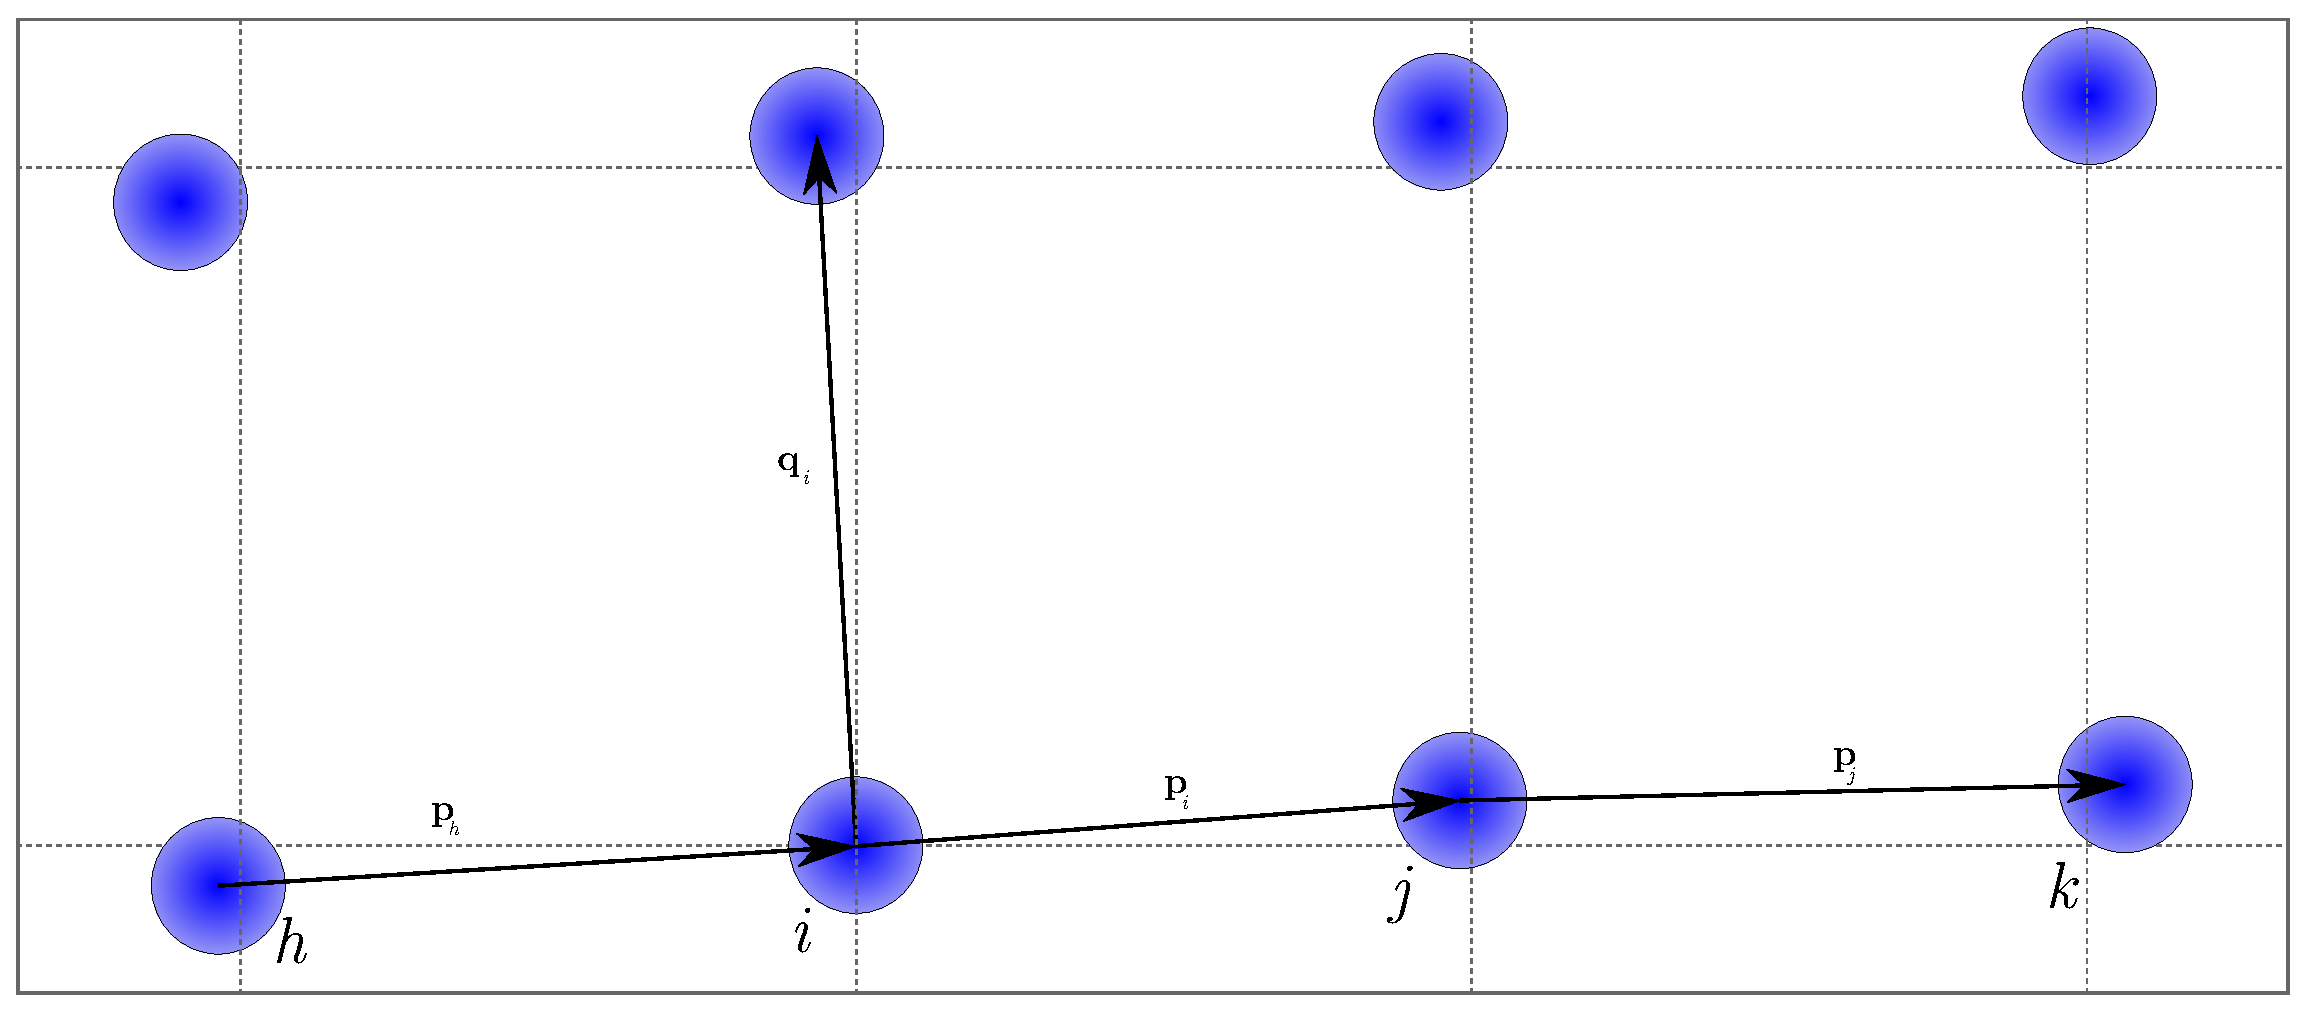
\includegraphics[width=\textwidth]{bonds}
\caption[Strained bonds in a dislocated crystal.]{The bonds that are considered for the $i$th atom in a region of crystal away from the slip plane; there is one bond to the nearest neighbour in the positive $x$~direction, $\mathbf{p}_i$, and one to the nearest neighbour in the positive $y$~direction, $\mathbf{q}_i$, to avoid double counting.\label{fig:bonds} }
\end{figure}





However there is a problem with this formulation. This assumes that every bond would, in equilibrium, be parallel to either the $x$ or the $y$ axis. This assumption is valid for the original Peierls model in which only displacements parallel to the $x$ direction were considered but the logarithmic term here represents a change in lattice orientation with position. A more nuanced approach requires some estimate of the local lattice orientation, if this is not done then the logarithmic term in \autoref{eqn:displacements} will mean that the strain in each bond will diverge, increasing with increasing distance from the dislocation core, whereas in reality the strains must be largest at the core.

There are clearly many possible ways of estimating the local lattice resistance, one possible method is to take the ideal orientation of the bond parallel to the slip plane for a particular bond to be paralell to the bonds on either side, i.e. as shown in \autoref{fig:bonds} the ideal orientation of $\mathbf{p}_i$ would be  parallel to $(\mathbf{p}_h + \mathbf{p}_j)$. The ideal orientation for $\mathbf{q}_i$ can be taken to be at \SI{90}{\degree} to this. So $\mathbf{\hat{i}}$ and $\mathbf{\hat{j}}$ in \autoref{eqn:estimate_strains} can be replaced with 
\begin{align}
\mathbf{\hat{i}}' &= \frac{(\mathbf{p}_h + \mathbf{p}_j)}{|\mathbf{p}_h + \mathbf{p}_j|} \nonumber \\
\mathbf{\hat{j}}' &= {\mathbf{\hat{i}}' \times \mathbf{\hat{k}}}
\end{align}
and the strain tensor can be calculated for each atom/unit cell, and hence the strain energy for each unit cell.



\FloatBarrier
\subsection{Misalignment energy}
\FloatBarrier

At the slip plane there is clearly going to be a break down of method highlighted above. For an atom immediately below the slip plane the identification of the nearest neighbour above the slip plane is perhaps not obvious. If the bond is taken to be simply  to the nearest atom above the slip plane ambiguities can arise 
It is possible that there will be two atoms equally close above the slip plane and such a simple criterion can lead to some atoms being bonded more than once and some atoms not being bonded. 

Instead a less arbitrary and more predictable method is to use the initial positions and assume that the $i$th atom can be bonded to two atoms in the layer above the slip plane. Since initially the horizontal spacing between atoms is $b$ for all atoms the two atoms must be within an interval $x_i^0 - b < x \leq x_i^0 + b$, as shown in \autoref{fig:slip_plane}. The energy for atom $i$ can be estimated from the average of the two bonds $\mathbf{q}_{i,\text{b}}$ and $\mathbf{q}_{i,\text{f}}$

\begin{figure}
\centering
\begin{subfigure}{\textwidth}
\centering
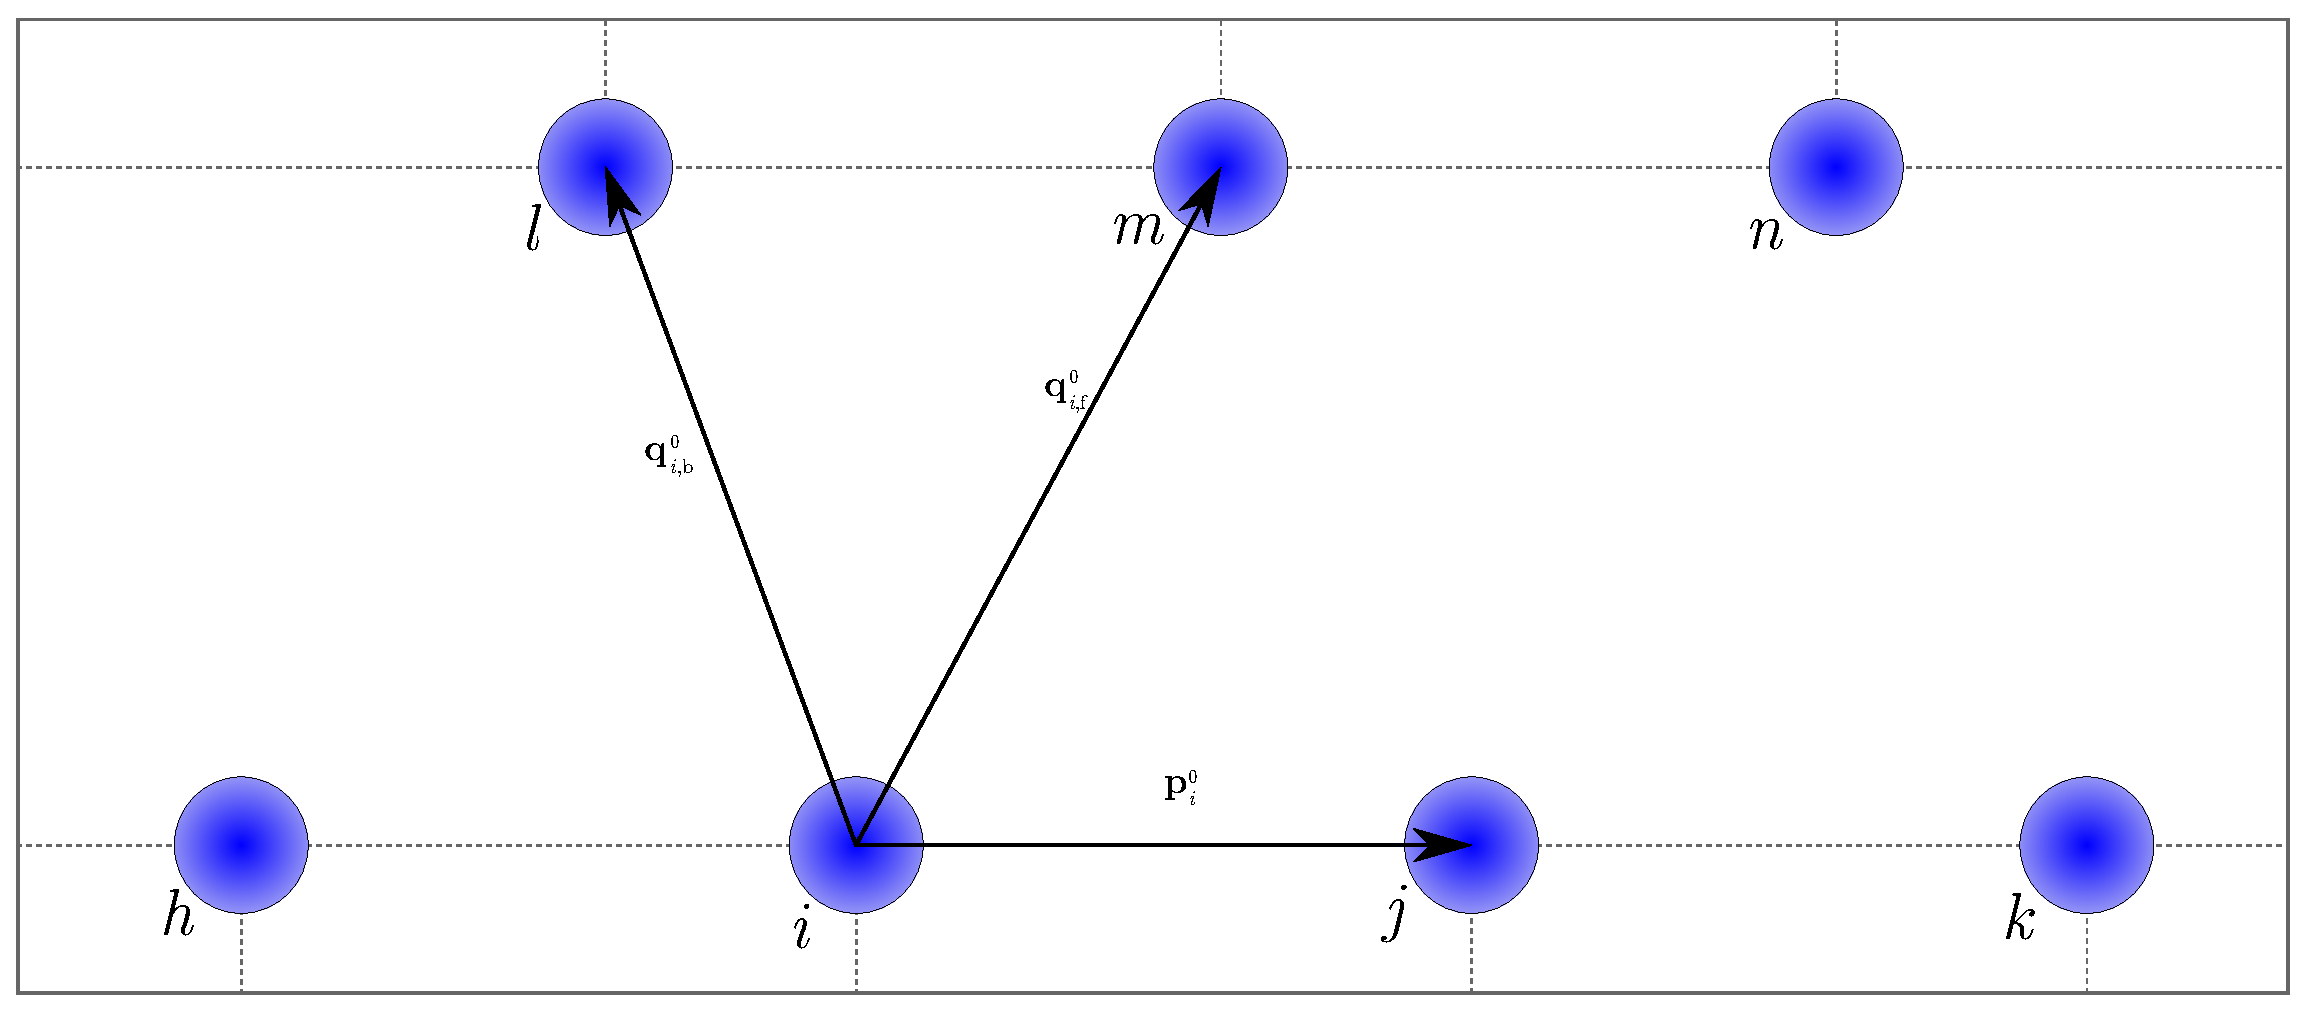
\includegraphics[width=\textwidth]{initial_slip_plane_bonds}
\caption{The initial positions of atoms either side of the slip plane.\label{fig:slip_plane_initial_positions}.}
\end{subfigure}
\par\medskip
\begin{subfigure}{\textwidth}
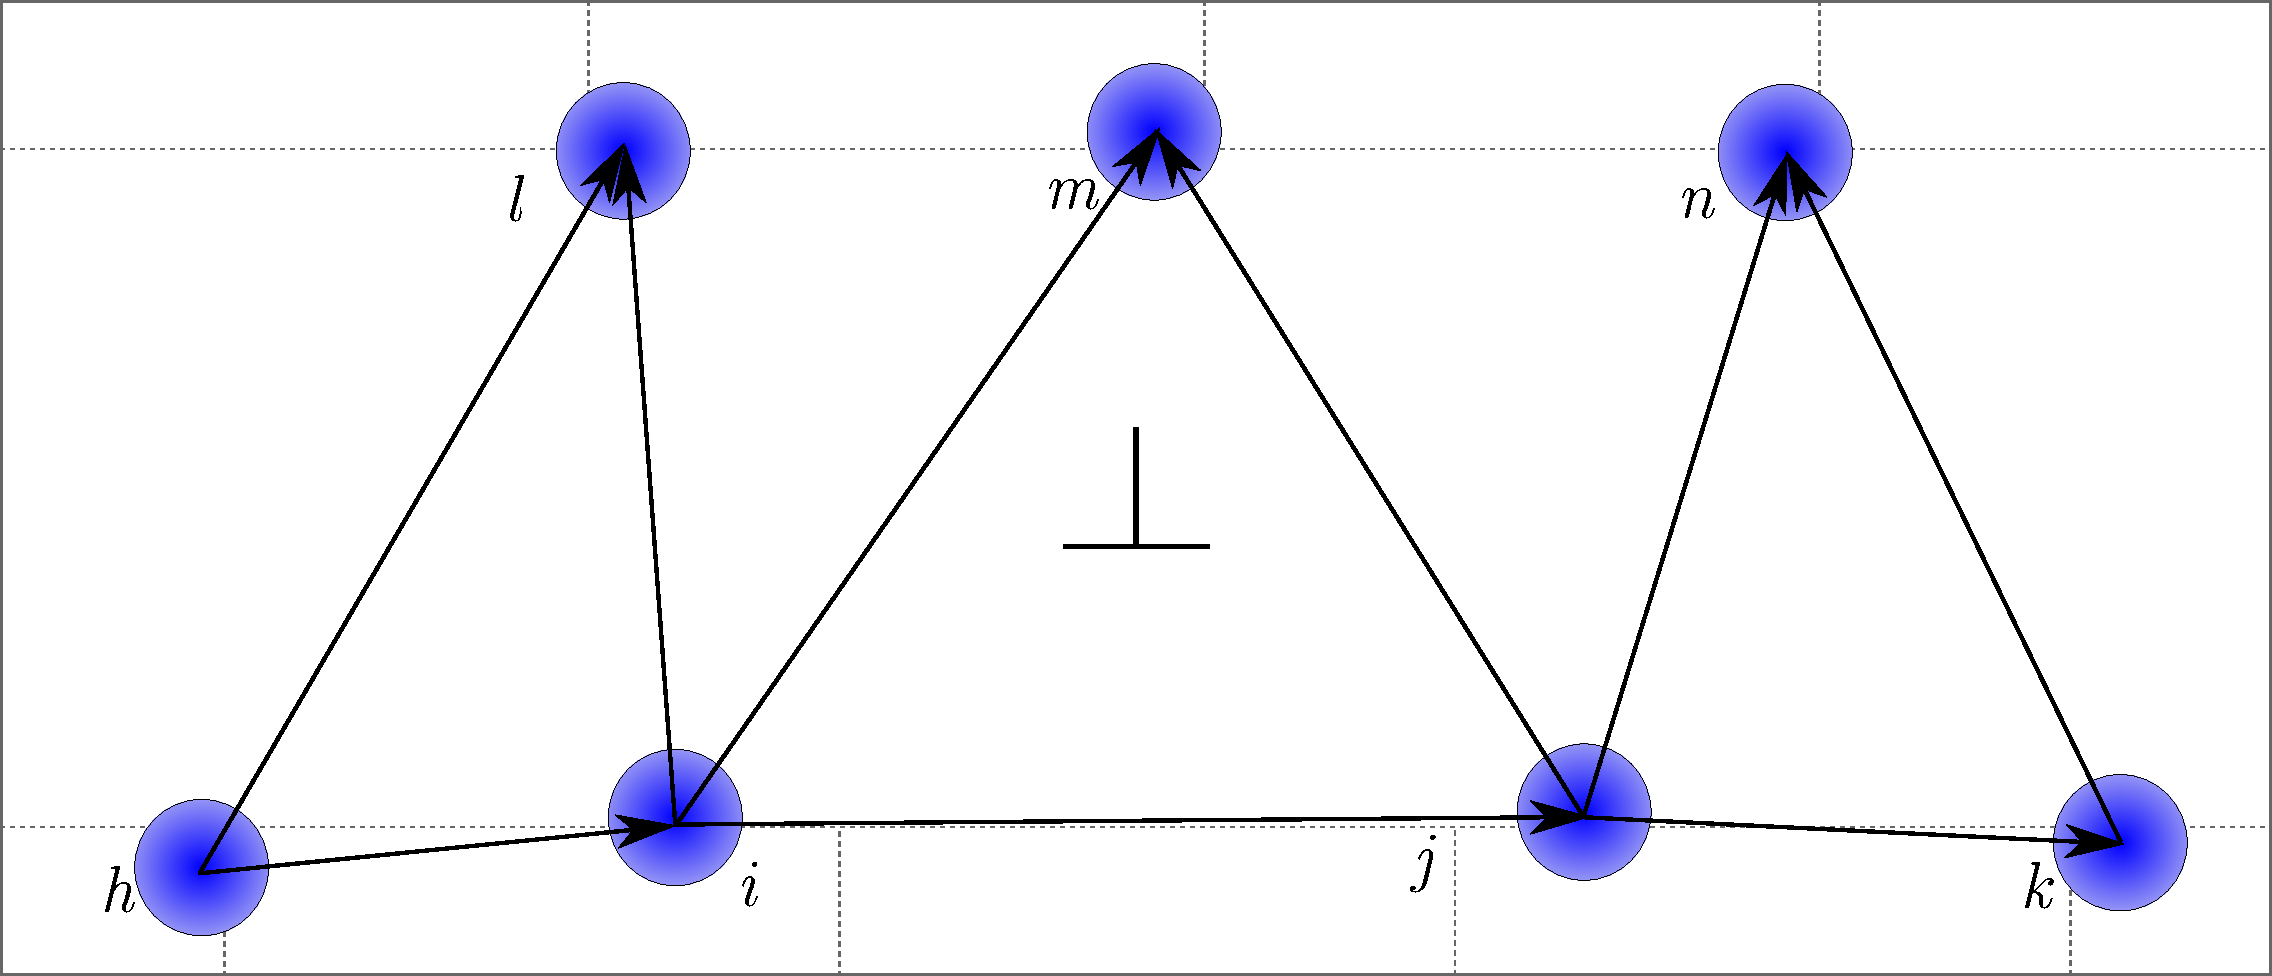
\includegraphics[width=\textwidth]{slip_plane_bonds}
\caption{The final positions of the atoms either side of the slip plane.\label{fig:slip_plane_final_positions}}
\end{subfigure}
\caption[Misaligned bonds cross the slip plane in a dislocated crystal.]{The slip plane before and after the application of the displacement field. The two atoms, $l$ and $m$, that can be considered bonded to the atom $i$ are shown along with the initial and final bonds, $\mathbf{q}_{i,\text{b}}$ and $\mathbf{q}_{i,\text{f}}$ which are backwards and forwards in the $x$ direction respectively. Also shown are the bonds $\mathbf{p}_h$ and $\mathbf{p}_j$ which are required to estimate the local orientation of the slip plane. \label{fig:slip_plane}}
\end{figure}


There are several methods to calculate the misaligned bonds. The simplest is to use the Frenkel approximation which, for an isotropic elastic material is 
\begin{equation}
U_i^\text{mis} = \frac{Gb^2}{4\pi^2} \left[\frac{d}{b}\right] \left[ 1 - \cos \left( \frac{2 \pi \phi}{d} \right) \right]
\end{equation}

which in terms of single crystal elastic constants takes $G=C_{66}$ (in Voigt notation see \cite{kelly_knowles2012chapter6_stress_strain}).

A more complete method for the calculation of the energy is to use the generalised stacking fault energy. Density functional theory can be used to calculate the energy of a stacking fault at an arbitrary misalignment. This is calculated by applying a displacement to two half crystals in a DFT simulation with periodic boundary conditions which introduces two opposing planar faults. The displacement is applied along the Burgers vector and the atoms are allowed to relax perpendicular to that displacement. Although the displacement field does not include any lateral (i.e. parallel to the lone vector) motion, allowing the DFT simulation of the stacking faults to relax laterally means that the energetic implications of lateral motion are included in the misalignment potential, although with an implicit assumption that the strains along the line vector do not extend beyond the slip plane. 

The energy changes with respect to a perfect crystal were considered and fitted with a simple empirical function:
\begin{equation}
\gamma(\phi) = \sum^{M}_{m=1} C_m \left[ 1 - \cos \left( \frac{2m\pi \phi}{b} \right) \right]
\end{equation}
where $\phi$ is the misalignment in the same units as the Burgers vector $b$, $m$ is an integer from \num{1} to $M$ and $C_m$ are coefficients fitted by a least-squares method to the energies calculated by DFT for different values of $\phi$. This is in units of \si{\joule\per\square\meter}, so a factor of $b$ must be applied to convert to a line energy in \si{\joule\per\meter}.


%%%%%%%%%%%%%%%%%%%%%%%%%%%%%%%%%%%%%%%%%%%%%%%%%%%%%%%%%%%%%%%5555%%%%%%%%%%%%%%%%%%%%%%%%%%%%%%%%%%%%%%%%%






%%%%%%%%%%%%%%%%%%%%%%%%%%%%%%%%%%%%%%%%%%%%%%%%%%%%%%%%%%%%%%%%%%%%%%%%%%%%%%%%%%%%%%%%%%%%%%%%%%%




\subsection{Empirical potentials}

Some materials can be described in a more physically insightful way than linear elasticity; as described in \autoref{sec:empirical_potentials}, empirical potentials have been developed for the field of molecular dynamics to be computationally convenient while at the same time approximating reality to a sufficient degree to gain insight into a system \cite{martinez2013}. One way to incorporate such potentials into the Peierls model described here is to write a simple python implementation of the potentials using the SciPy and NumPy packages and associated tools \cite{Numpy2011,Ipython2007,Millman2007,SciPy2001}; another way is to use the Atomic Simulation Environment \cite{ASE2017} or the python interface to the LAMMPS software package \cite{Plimpton1995,LAMMPS_web}.



To demonstrate the principle of using more physically informed potentials and hopefully capture more details of the energy changes as dislocations move the ionic solids were investigated using the Lennard-Jones potential:
\begin{equation}
\phi_{ij}(r_{ij}) = 4\epsilon_{ij} \left[ \left( \frac{\sigma_{ij}}{r_{ij}}\right)^{12}-     \left( \frac{\sigma_{ij}}{r_{ij}}\right)^6   \right]
\end{equation}
where $\epsilon_{ij}$ is the depth of the energy well and $\sigma_{ij}$ is the radius at which the energy is equal to zero or in the A--B form:
\begin{equation}
\phi_{ij}(r_{ij}) = \frac{A_{ij}}{r_{ij}^{12}} - \frac{B_{ij}}{r_{ij}^{6}}
\end{equation}
where $A_{ij} = 4\epsilon_{ij}\sigma_{ij}^{12}$ and $B_{ij} = 4 \epsilon_{ij} \sigma_{ij}^{6}$. The energy for any two atoms is then 
\begin{equation}
U_{ij}(r_{ij}) = \frac{1}{4\pi\epsilon_0} \frac{q_i q_j}{r_{ij}} + \frac{A_{ij}}{r_{ij}^{12}} - \frac{B_{ij}}{r_{ij}^{6}}
\end{equation}
where $\epsilon_0$ is the permittivity of free space.

The Lennard-Jones has been chosen as a simple example to demonstrate the application of empirical potentials for which fitted parameters are readily available \cite{Mao2014} and applicable to a class of materials for which the dislocation properties are not well explained by linear elasticity, the alkali halides.



\begin{table}
\centering
  \begin{tabular}{| m{3cm} | d{4} | d{-1} |}
  \hline
   Ion \rule{0pt}{3ex} & \multicolumn{1}{c|}{$\sigma_i$/\si{\angstrom}} & \multicolumn{1}{c|}{$\epsilon_i$/\si{\joule\per\mole}  }\\ \hline
   \ce{Li+} \rule{2ex}{0pt} & 1.715 & 241.25 \\
   \ce{Na+} & 2.497 & 327.44 \\
   \ce{K+} & 3.184 & 494.97 \\
   \ce{Rb+} & 3.302 & 1006.25 \\
   \ce{Cs+} & 3.440 & 2097.44 \\
   \ce{F-} & 3.954 & 27.05 \\
   \ce{Cl-} & 4.612 & 104.68 \\
   \ce{Br-} & 4.812 & 150.46  \\
   \ce{I-} & 5.197  & 176.56 \\
  \hline
  \end{tabular}
\caption[Lennard-Jones parameters.]{\rule[3ex]{0pt}{0pt} Parameters used for Lennard-Jones calculations from \cite{Mao2014}.\label{tab:LJ_params}}
\end{table}


The parameters used for the Lennard-Jones potential are shown in \autoref{tab:LJ_params}. They are calculated for each ion individually, to best reproduce lattice properties, and must be combined according to Lorentx-Berthelot rules:
\begin{align}
\epsilon_{ij} &= \sqrt[]{\epsilon_i \epsilon_j} \nonumber\\
\sigma_{ij} &= \frac{\sigma_i + \sigma_j}{2}
\end{align}

A na\"{\i}ve brute force implementation is given in Section~\ref{sec:ionic_energy_code} and an example input file is given for LAMMPS in Section~\ref{sec:lammps_input}. The LAMMPS pair style used was ``\texttt{lj/long/coul/long}'', the parameters for which are given in the example input file and is described in the LAMMPS documentation in \cite{LAMMPS_web}.

\subsection{Optimisation of the dislocation structure}
\label{sec:optimisers}
Given one of the above cases, or a similar one, that provides energy as a function of a small number of parameters, an optimisation routine is required. The original version of this Peierls model included a simple binary search algorithm to find the width of the dislocation. However for a multi-parameter space this is not appropriate.

Fortunately the open source project SciPy has a number of optimisers built in. The one chosen was the quasi-Newton method of Broyden, Fletcher, Goldfarb, and Shanno \citep{SciPy2001,nocedal2006}, or BFGS. This method uses the first derivative, methods such as this are known as hill-climbing optimisers, seeking a stationary point.

While the derivative of the energy with respect to the parameters is not simple to find, the atomic positions are defined as smooth functions of the input parameters and the energy is (at least likely to be) a smooth function of the atomic positions. Hence the overall behaviour of the energy as a function of the input parameters should be well suited to a gradient based method. The SciPy implementation of the BFGS algorithm includes the ability to approximate the first derivative numerically.

If it is found that the energy function is not well behaved SciPy also includes the Nelder-Mead simplex algorithm that does not make use of gradient information. This method calculates the objective function, here the energy, at $n+1$ points in parameter space where $n$ is the number of parameters. This defines a ``simplex'', i.e. a triangle in two dimensions, a tetrahedron in three and so on. A search direction is defined along the vector joining the worst of these $n+1$ points and the centroid of the rest, and a small number of point along this line are trialled. The worst point of the initial simplex is then replaced and the process repeated \citep{Nelder1965,Gao2012}.




























































\section{Results and Discussion}

\subsection{Elastic Energy Calculations}
\label{sec:elastic_results}

The equilibrium dislocation configuration for a given dislocation position was calculated by optimisation of the dislocation structure with respect to the calculated energy, the sum of the strain energy in the half crystals either side of the slip plane and the misalignment energy in the slip plane. As discussed in section~\ref{sec:optimisers} the choice of optimiser is affected by the behaviour of the function. The BFGS was found to be faster than the Nelder-Mead, though both algorithms produced very similar results, within the tolerance (i.e. the error that can be tolerated) set for the algorithms to terminate. It was found that only a very small error in the result could be tolerated in deciding the algorithm had converged. Tolerating larger errors led to inconsistent results. A relative error of around \num{1e-7} was usually sufficiently low. This is important because small changes in the energy are being studied. 

The variation of the dislocation energy with respect to the dislocation parameters, as defined in \autoref{eqn:displacement_field}, was investigated. These calculations were performed for a dislocation in copper at $\alpha=0$. The simulation cell used extended to \num{800} Burgers vectors from the dislocation core, which is approximately \SI{0.4}{\micro\meter} across the whole simulation.

First the dislocation structure was optimised to find the equilibrium configuration, then the  various parameters were varied away from these equilibrium values individually. The results are shown in \autoref{fig:variation_of_U_with_params}. 


\begin{figure}
\centering
\begin{subfigure}{0.4\textwidth}
\centering
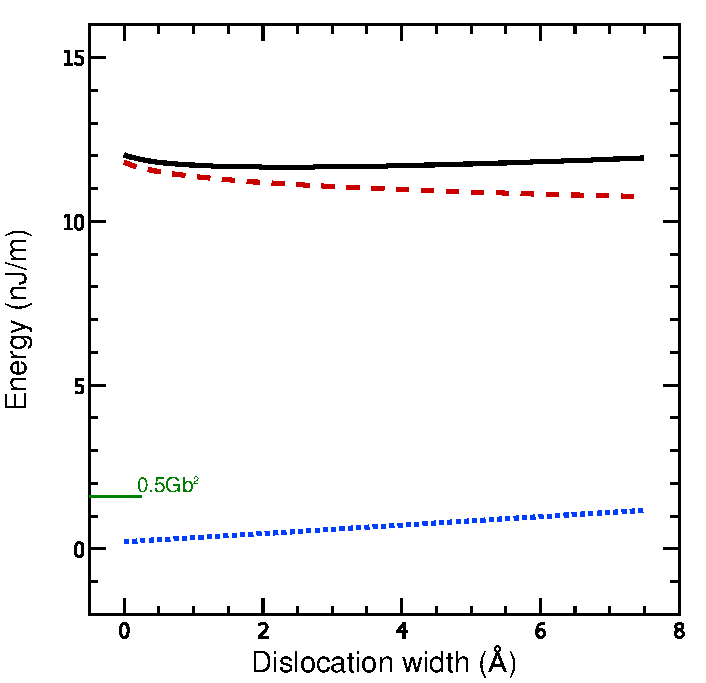
\includegraphics[width=\textwidth]{U_vs_w}
\caption{The variation in the dislocation energy with the dislocation width.\label{fig:U_vs_w}}
\end{subfigure}
~
\begin{subfigure}{0.4\textwidth}
\centering
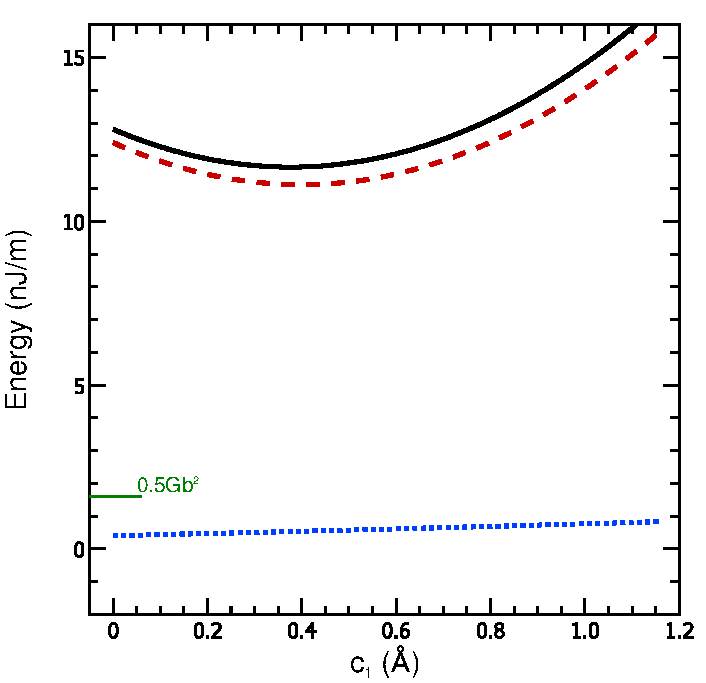
\includegraphics[width=\textwidth]{U_vs_c1}
\caption{The variation in the dislocation energy with the dislocation parameter $\mathbf{c_1}$.}
\end{subfigure}

\begin{subfigure}{0.4\textwidth}
\centering
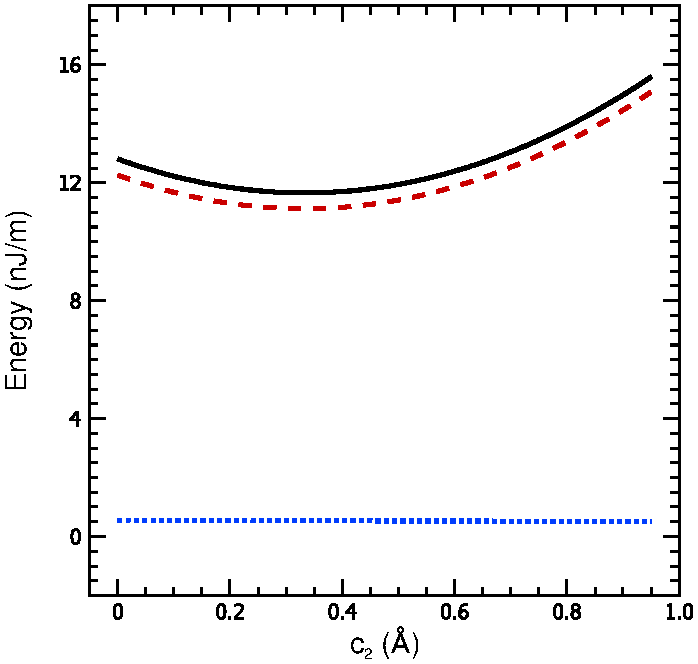
\includegraphics[width=\textwidth]{U_vs_c2}
\caption{The variation in the dislocation energy with the dislocation parameter $\mathbf{c_2}$.}
\end{subfigure}
~
\begin{subfigure}{0.4\textwidth}
\centering
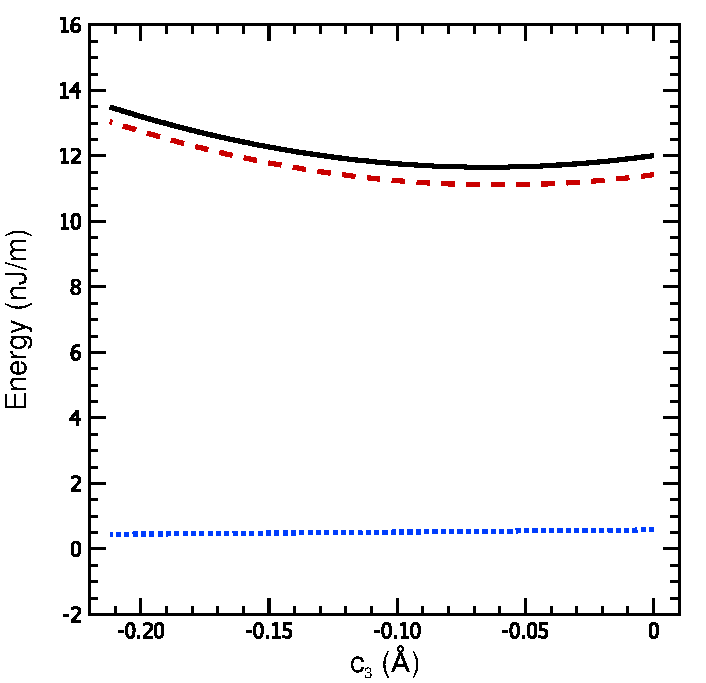
\includegraphics[width=\textwidth]{U_vs_c3}
\caption{The variation in the dislocation energy with the dislocation parameter $\mathbf{c_3}$.}
\end{subfigure}
\captionsetup{width=0.9	\textwidth,font={sf,scriptsize},labelfont=bf}
\caption[The variation of the line energy with the displacement parameters.]{The variation of the calculated energy of a dislocation in copper at the $\mathbf{\alpha=0}$ position, calculated for a simulation extending \SI{0.4}{\micro\meter} from the dislocation core. The parameters are as defined in \autoref{eqn:displacement_field}. Only one parameter was varied at a time, all the others were held constant at their equilibrium values. The total energy is the solid black line, the strain energy in the two half crystals is the dashed red line and the misalignment energy in the slip plane is the dotted blue line. \label{fig:variation_of_U_with_params}}
\end{figure}


\begin{table}


\centering
\begin{tabular}{ l c c c }
\hline
\rule[2.5ex]{0pt}{0pt}Parameter                & Ideal             & Simulated $\alpha=0$  & Simulated $\alpha=0.5$  \\
\hline
$w$ (\si{\angstrom})  \rule[2.5ex]{0pt}{0pt}   & 1.581             & 2.441                 & 2.431 \\
$c_1$ (\si{\angstrom})                         & 0.308             & 0.36268                & 0.36270 \\
$c_2$ (\si{\angstrom})                         & 0.308             & 0.293070               & 0.293075 \\
$c_3$ (\si{\angstrom}) \rule[-0.5ex]{0pt}{0pt} & -0.0493           & -0.061864               & -0.061862 \\
Energy (\si{J/m})                              &  \num{1.56795e-9} & \num{1.20965e-08}      & \num{1.20963e-08} \\
\hline
\end{tabular}
\caption[A comparison between the ideal and simulated dislocation parameters]{A comparison of the ideal dislocation parameters and those found by optimising the energy of a simulated dislocation, the ideal values of $c_1$, $c_2$, $c_3$ and $w$ are calculated from the elastic constants using \autoref{eqn:expressions_for_the_ideal_disloca_parameters}. The ideal energy is taken to be $^1\!/_2 Gb^2$.\label{tab:dislocation_params}}
\end{table}

As expected all the parameters showed a single minimum and the variation was smooth, so a variational approach is applicable and the optimiser is likely to be reliable, i.e. the lowest energy configuration can be said to be the configuration a dislocation would take. 






The values of these parameters have simple solutions for the case of an isotropic elastic medium, given in \autoref{eqn:half_width} and \autoref{eqn:expressions_for_the_ideal_disloca_parameters}. These only depend on the Poisson's ratio, which for copper is \num{\sim0.34} \cite{Koster1961}, and the lattice parameters. These ideal values are compared with the optimised values in \autoref{tab:dislocation_params}. The energy of the dislocation is approximately $4Gb^2$, higher than the $\sim0.5 G b^2$ that might be expected. However the values of the dislocation configuration parameters are similar to the ideal values, as calculated from \autoref{eqn:expressions_for_the_ideal_disloca_parameters}. The atomistic model differs from the isotropic elastic continuum in that the values of the parameters vary as a function of $\alpha$ and the symmetry between $c_1$ and $c_2$, which are equal for an isotropic material, is broken.

The small variations in the values of the dislocation parameters and the dislocation energy, both as relative and absolute values, require that care is taken in the computation not to introduce errors. One example that has already been mentioned is the tolerance, or relative error that can be tolerated before the optimisation is terminated. If the tolerance is not tight enough,  this manifests as noise that depends on the initial guess to start the optimisation search, or the exact choices of parameters in the optimisation algorithm. This apparent noise would be deterministic but unpredictable so would to appear random. 

Another problem was the precision of the floating point arithmetic. It was found that \num{64} bit precision was usually sufficient, but some systems had such drastically different magnitudes for the strain and misalignment energies that the sum rounded to the strain energy. The dislocation energy would then be wrongly optimised to reduce that term alone. While the strain energy term dominated the line energy for these materials, principally silicon, the changes in the misalignment energy and the changes in the strain energy term were not nearly as different as the values themselves. The problem was addressed by using NumPy's \num{128} bit precision.  





\begin{figure}
\centering
% \begin{subfigure}{\textwidth}
% \centering
% 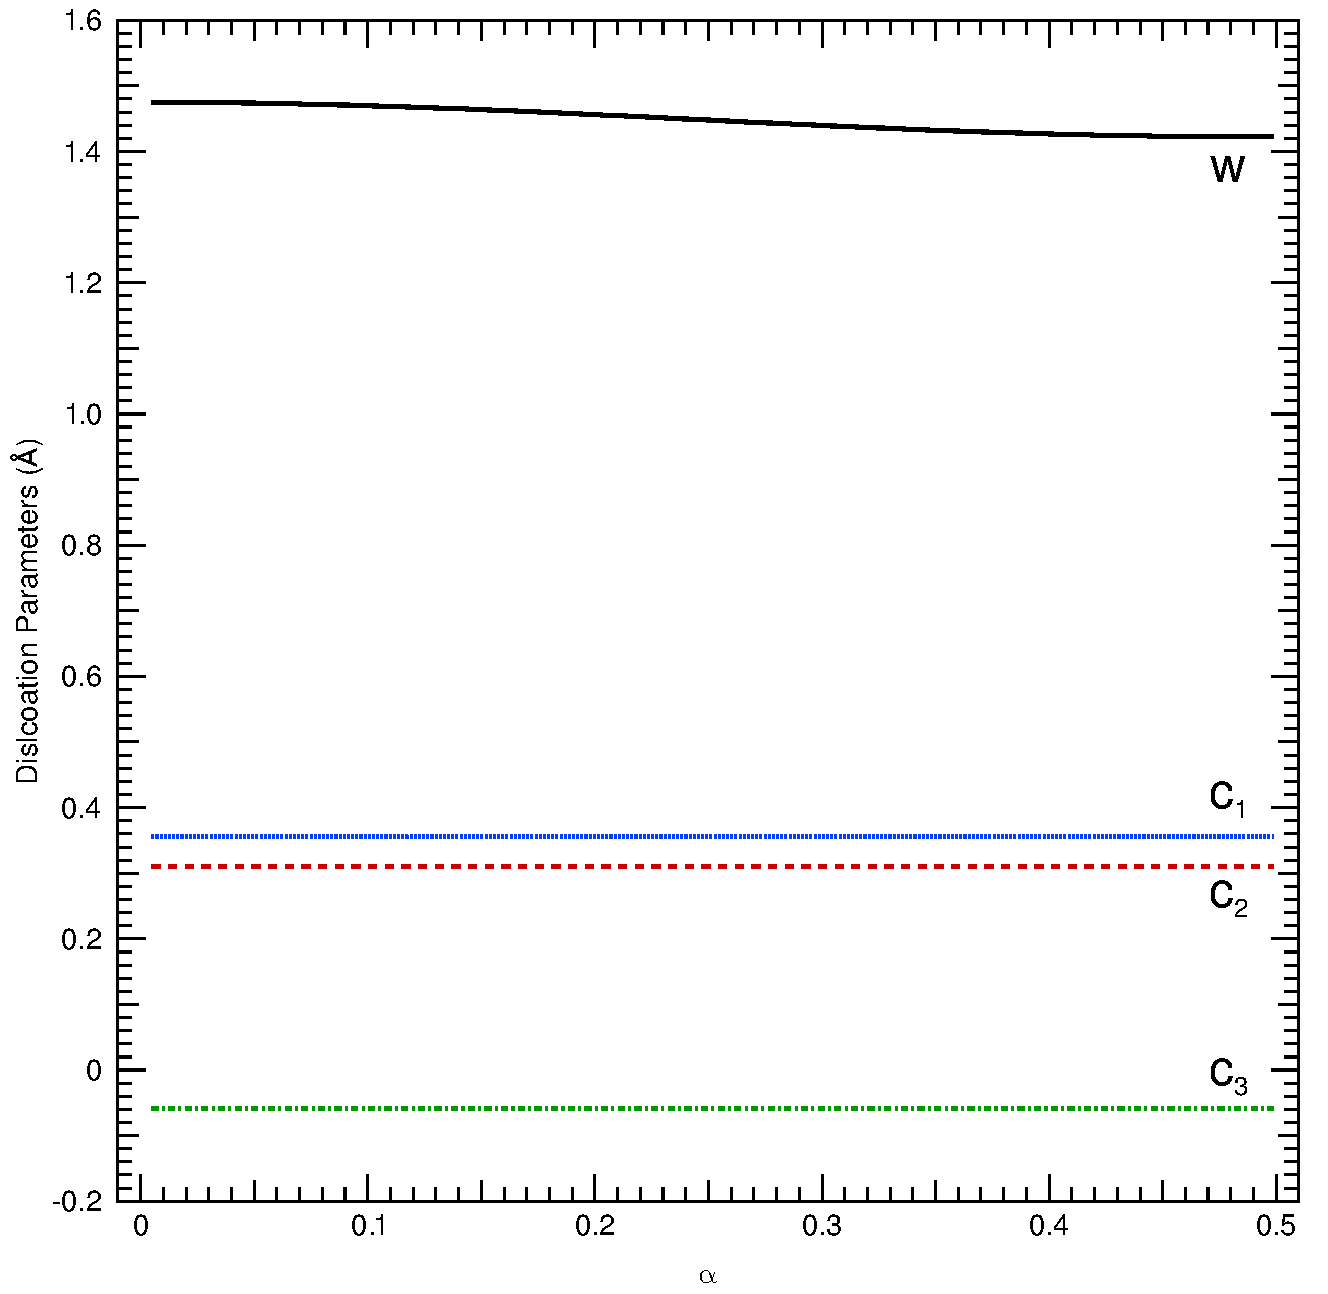
\includegraphics[width=0.6\textwidth]{disloc_params_vs_alpha}
% \caption{The variation of the dislocation configuration parameters, $\mathbf{w}$, $\mathbf{c_1}$, $\mathbf{c_2}$ and $\mathbf{c_3}$, as a function of $\mathbf{\alpha}$.}
% \end{subfigure}

\begin{subfigure}{0.45\textwidth}
\centering
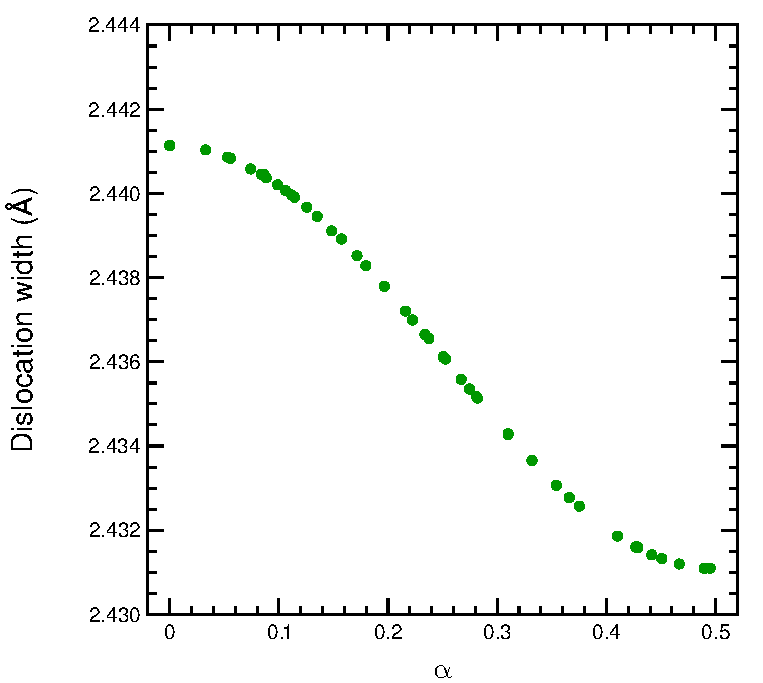
\includegraphics[width=\textwidth]{w_vs_alpha}
\caption{The variation of the dislocation width, $w$, as a function of $\alpha$. The width defines the region of the slip plane where the misalignments are greater than half the maximum value.}
\end{subfigure}
~
\begin{subfigure}{0.45\textwidth}
\centering
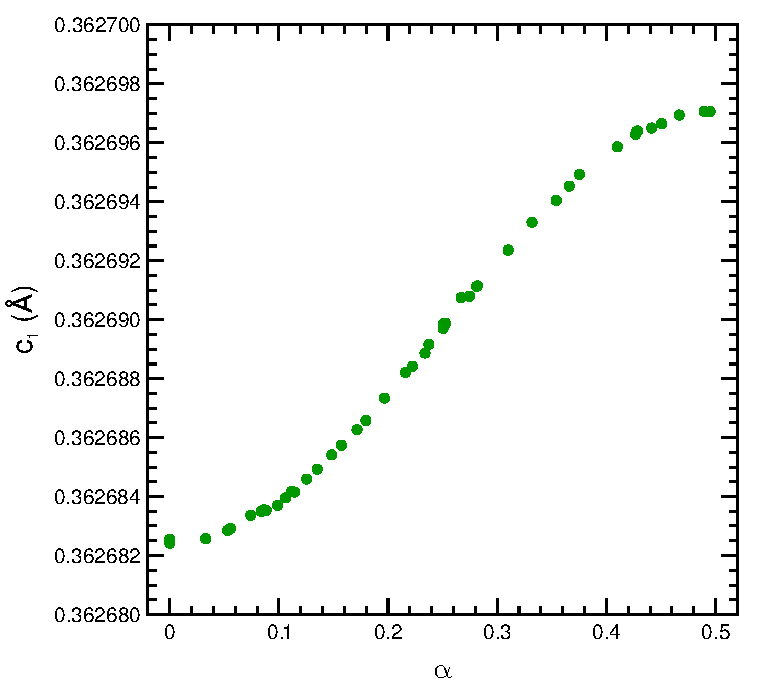
\includegraphics[width=\textwidth]{c1_vs_alpha}
\caption{The variation of the dislocation width, $c_1$, as a function of $\alpha$. The parameter $c_1$ represents the magnitude of the $xy$ strains.\rule[-\baselineskip]{0pt}{0pt}}
\end{subfigure}

\begin{subfigure}{0.45\textwidth}
\centering
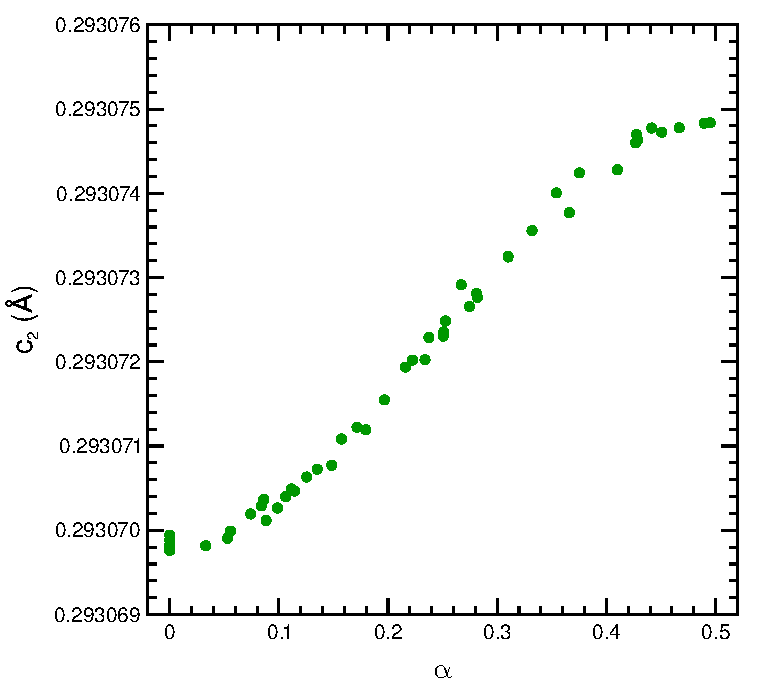
\includegraphics[width=\textwidth]{c2_vs_alpha}
\caption{The variation of the dislocation width, $c_2$, as a function of $\alpha$. The parameter $c_2$ represents the magnitude of the $yx$ strains.\rule[-\baselineskip]{0pt}{0pt}\label{fig:c2_vs_alpha}}
\end{subfigure}
~
\begin{subfigure}{0.45\textwidth}
\centering
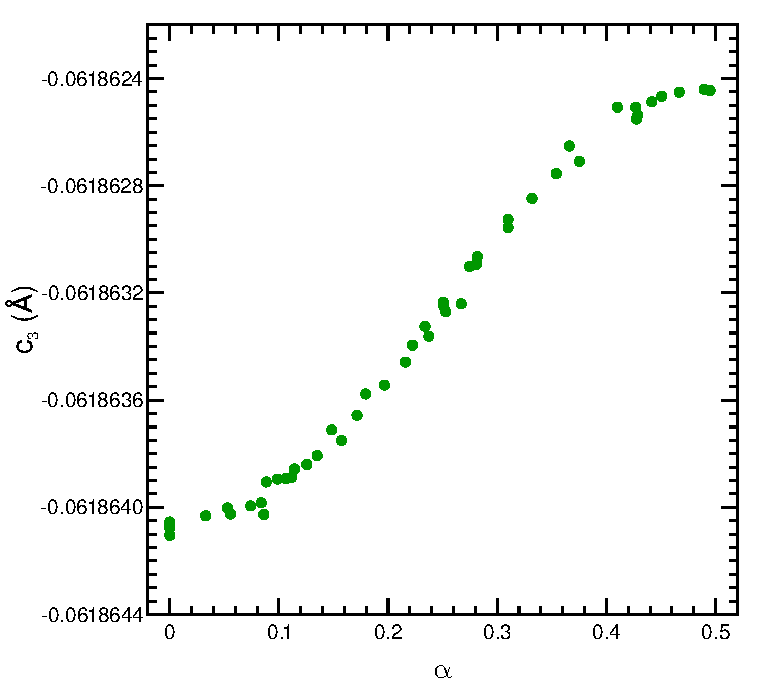
\includegraphics[width=\textwidth]{c3_vs_alpha}
\caption{The variation of the dislocation width, $c_3$, as a function of $\alpha$. The parameter $c_3$ represents the magnitude of the bending that arises in a crystal as a result of the introduction of an extra half plane of atoms.}
\end{subfigure}

\caption[The variation of the displacement parameters with dislocation position.]{The variation of the displacement field configuration parameters with $\mathbf{\alpha}$. Only small changes in the parameters were seen, the largest changes were seen in $w$ and the smallest in $\mathbf{c_3}$. The parameter all vary smoothly and approach $\mathbf{\alpha=0, 0.5}$ with no gradient, as required for equilibrium. Some noise was observed in the value of $\mathbf{c_2}$ and $\mathbf{c_3}$. \label{fig:disloc_params_vs_alpha}}
\end{figure}


The variation of the dislocation parameters and the dislocation energy were investigated by randomly sampling $\alpha$ in the range \numrange{0}{0.5} and optimising the dislocation configuration to give the lowest energy. The variation in the dislocation configuration parameters is given in \autoref{fig:disloc_params_vs_alpha}, while the variation of the total energy is given in \autoref{fig:Copper_U_tot_vs_alpha} and the relative changes in the different energy components is shown in \autoref{fig:copper_800_rel_energies}.

An important observation is that the periodicity of the dislocation energy, and indeed the dislocation configuration, predicted by this model is $b$, not $^b\!/_2$ as predicted by \citet{Peierls1940,Clegg2006}. As discussed in Chapter~\ref{chap:plastic_deformation}, this is expected based on the symmetry inherent in the model. 

Peierls introduced an implicit symmetry by assuming that the dislocation configuration does not change as the dislocation moves and thus predicted a period of $^b\!/_2$. The formulation was changed by \citet{Huntington1955} to predicted a period of $b$. The model presented by \citet{Clegg2006} included an implicit symmetry since motion of atoms was limited to the slip direction and the strain energy was calculated from strains in the atomic bonds rather than as an integral over an elastic medium. This meant that there was no distinction between the atoms above the slip plane and the atoms below the slip plane, and thus no distinction between the $\alpha = 0$ and $\alpha = 0.5$ position. The current model has no such symmetry across the slip plane, due to the logarithmic term in \autoref{eqn:displacement_field}, and so the periodicity of $b$ is expected.

The dislocation parameters vary smoothly from $\alpha = 0$ to $\alpha = 0.5$ and approach the two equilibrium positions with zero gradient as required by equilibrium. There is some noise in the value of $c_2$, as shown in \autoref{fig:c2_vs_alpha}. This is likely due to the changes in the dislocation parameters being close to the tolerance of the optimisation algorithm. This is not sufficiently noisy to present a problem, but highlights the need for care in deciding the trade off between computational time and the accuracy of the calculated values.



\begin{figure}
\captionsetup{width=0.6\textwidth,font={sf,scriptsize},labelfont=bf}
\centering
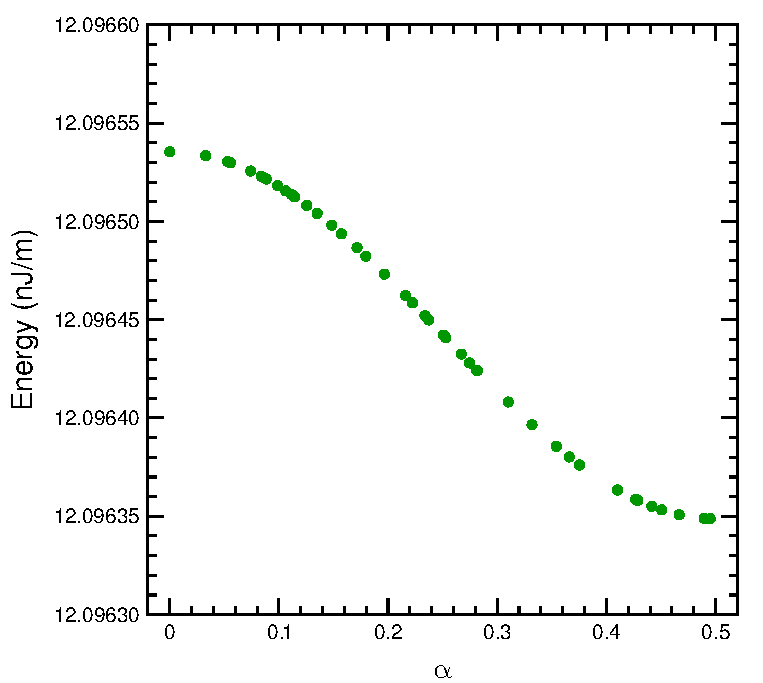
\includegraphics[width=0.5\textwidth]{Copper_800_U_tot}
\caption[Energy variation of a dislocation in copper with the dislocation position.]{The variation of the dislocation energy with position for a dislocation in copper. The results shown are for a model including atoms to a distance of 800 Burgers vectors from the dislocation core, i.e. a distance of $\sim$\SI{300}{\nano\metre}.  Note that the changes in energy are small relative to the absolute value of the dislocation energy, at around \num{1e-5}\,$U_{\text{disloc}}$.\label{fig:Copper_U_tot_vs_alpha}}
\end{figure}

The variation of the energy with $\alpha$, \autoref{fig:Copper_U_tot_vs_alpha}, was qualitatively as expected from previous work \cite{Bulatov1997,Clegg2006}: a smooth but very small variation in the energy, some five orders magnitude smaller than the value of the dislocation energy. The variation of the two components of the energy was also as expected. This is most easily seen as changes by setting the energy at $\alpha=0$ to be zero, as shown in \autoref{fig:copper_800_rel_energies}. The strain energy and the misalignment energy vary out of phase with each other, thus the two components of the energy experience larger variations than the total. It is also possible that the relative magnitude of the two components will alter which of the two equilibrium positions is stable and which is unstable.


\begin{figure}
\captionsetup{width=0.6\textwidth,font={sf,scriptsize},labelfont=bf}
\centering
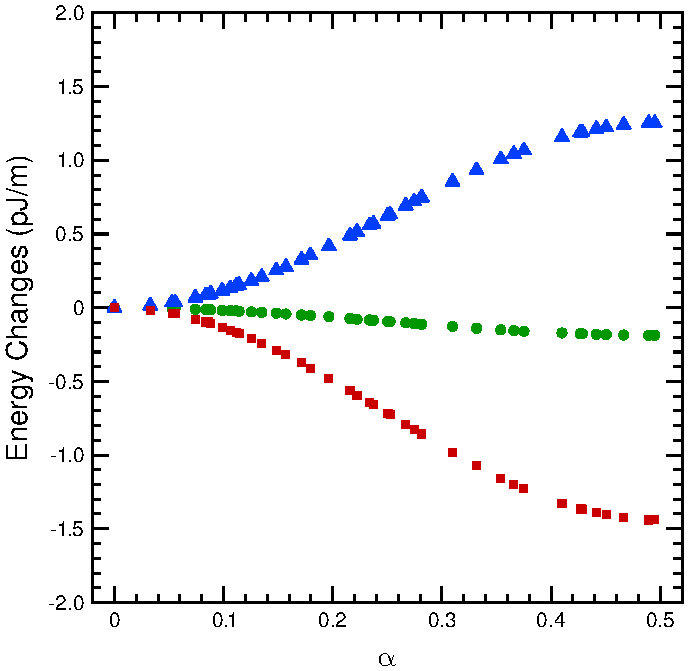
\includegraphics[width=0.5\textwidth]{Copper_800_rel_energies}
\caption[The energy changes with dislocation position for  copper.]{The energy changes with position for a dislocation in copper showing the two components of the energy, the strain energy and the misalignment energy, and the total energy. This simulation extended \num{800} Burgers vectors from the dislocation core, or around \SI{04}{\micro\meter}.\label{fig:copper_800_rel_energies}}
\end{figure}




To undertake further analysis the energy variation can be fitted with a simple empirical function:
\begin{equation}
U = \sum^N_n C_n \cos (2 \pi n \alpha) \label{eqn:empirical_function}
\end{equation}
where $C_n$ are the parameters to be fitted, $n$ is an integer between $0$ and $N$ and $\alpha$ is the displacement of the dislocation from the initial position as a fraction of the Burgers vector. Usually it was found that $N=4$ gave a good fit to the calculated energy variations. Since this is an easily differentiable function, the stress can be calculated in a straightforward manner from the gradient:
\begin{equation}
\tau = \frac{dU}{d\alpha} \frac{1}{lb^2}
\end{equation}
where $l$ is the length of dislocation line and $b$ is the Burgers vector. The gradient is readily calculated by
\begin{equation}
\frac{dU}{d\alpha} = \sum_n^N - 2 \pi C_n \sin ( 2 \pi n \alpha )
\end{equation}

This provides a smooth and differentiable function that both allows for noise in the data and makes calculating the Peierls stress easier. The Peierls stress is the maximum value of the stress, which occurs at the point of maximum gradient $dU/d\alpha$, i.e. where
\begin{equation}
\frac{d^2U}{d\alpha^2} = \sum_n^N -4 \pi^2 n^2 C_n \cos ( 2 \pi n \alpha ) = 0
\end{equation}

A script was written to do this fitting and gradient calculation automatically; the code is included in an archive which can be found in \cite{code}. An example of this sort of fit is shown in \autoref{fig:empirical_fit}. For the example of copper above, this yields a Peierls stress of \SI{8.98}{\mega\pascal} or, as a fraction of the shear modulus, \num{2.54e-4}\,$G$. This is approximately 10 times larger than the value estimated by experiment \cite{Wang1996}. However for very soft materials the error in such experiments can be very large as other effects can be as large or larger than the estimated lattice resistance.

\begin{figure}
\centering
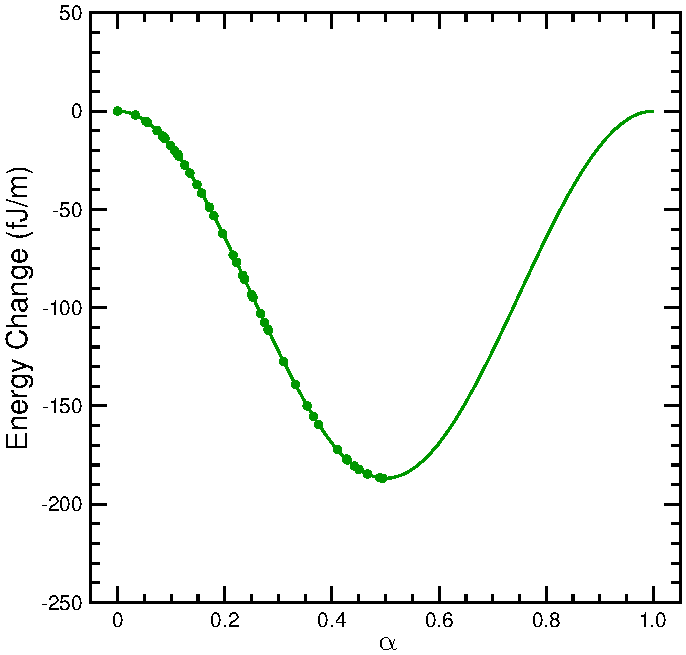
\includegraphics[width=0.5\textwidth]{Empirical_Fit}
\captionsetup{width=0.6\textwidth,font={sf,scriptsize},labelfont=bf}
\caption[Empirical fit to the variation in energy with dislocation position.]{Empirical fit to the dislocation energy as it varies with dislocation position using 4 terms. The fit is good, so can be reliably used for further analysis.\label{fig:empirical_fit}}
\end{figure}


To characterise the dependence of the model on the volume of crystal modelled, various simulation sizes were modelled for dislocations in copper. The size here is the range about the core of the dislocation in the slip direction and normal to the slip planes, while symmetry was exploited along the dislocation line to model only one repeat unit. The resulting simulated crystal therefore has a rectangular cross-section, rather than, say, cylindrical.

%Schematic?

\begin{figure}
\centering
\begin{subfigure}{0.4\textwidth}
\centering
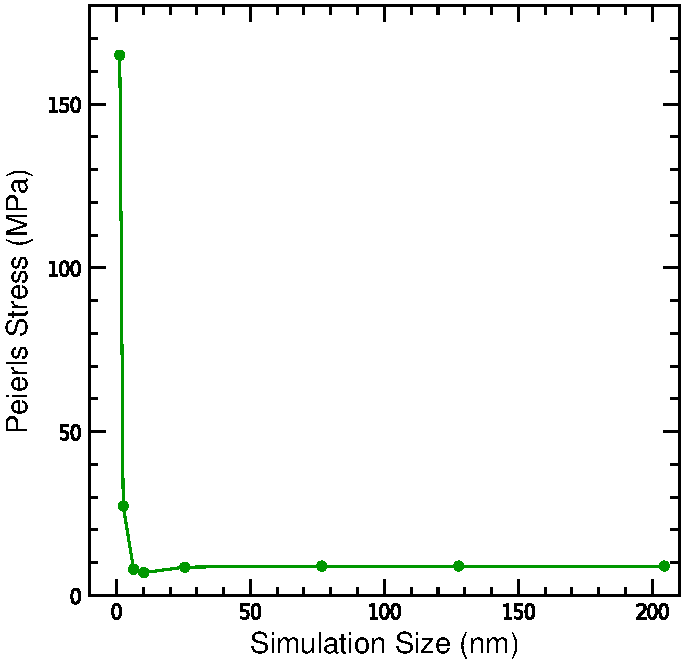
\includegraphics[width=\textwidth]{Tp_vs_size}
\caption{The variation of the calculated Peierls stress with simulation size.}
\end{subfigure}
~
\begin{subfigure}{0.4\textwidth}
\centering
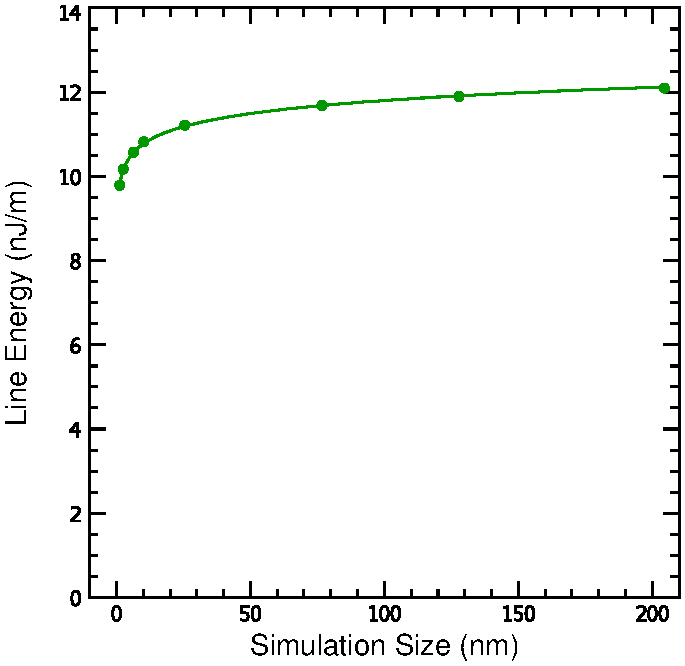
\includegraphics[width=\textwidth]{Energy_vs_size}
\caption{The variation of the calculated dislocation line energy with the simulation size and a best fit line for a logarithmic function.\label{fig:energy_vs_size}}
\end{subfigure}
\captionsetup{width=0.9\textwidth,font={sf,scriptsize},labelfont=bf}
\caption[The effect of simulation size on dislocation energy and Peierls stress.]{Plots characterising the sensitivity of the model to the simulation size. The value of the Peierls stress is quite quickly converged to a constant, the energy in fact increases logarithmically, as shown by the best fit line.\label{fig:effect_of_size_on_simulation}}
\end{figure}

\begin{figure}
\captionsetup{width=0.6\textwidth,font={sf,scriptsize},labelfont=bf}
\centering
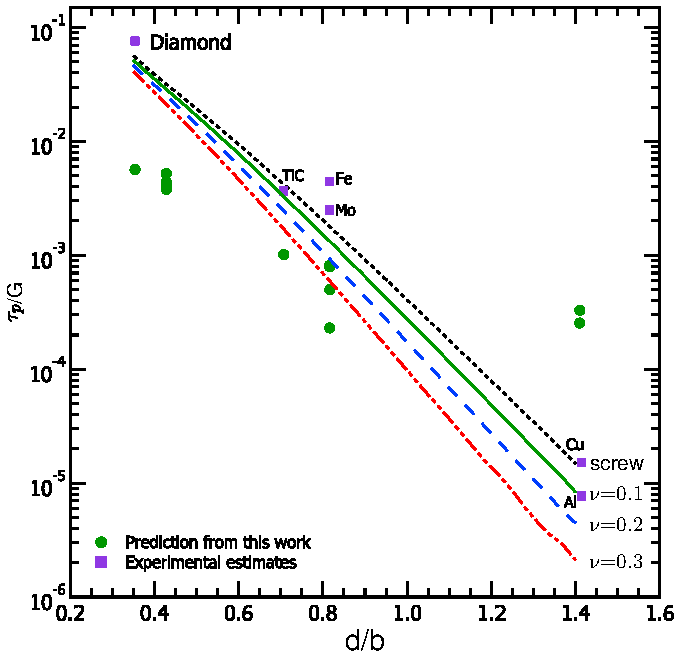
\includegraphics[width=0.5\textwidth]{tp_G_vs_d_b}
\caption[A comparison of predicted Peierls Stresses against previous estimates.]{A comparison of predicted Peierls Stresses against experimental estimates \cite{Wang1996} and a previous model \cite{Clegg2006} for an isotropic material, the highest for a screw dislocation and the others are for edge dislocations where $\nu=$ 0.1, 0.2 and 0.3. \label{fig:tp_vs_d_b}}
\end{figure}


The energy and Peierls stresses were calculated and are presented in \autoref{fig:effect_of_size_on_simulation}. The effects of size are limited to a small range for this elastic simulation, with the Peierls stress converging to \SI{1}{\percent} when the simulation is  \SI{\sim 30}{\nano\meter} across, which is around a hundred Burgers vectors.

The variation of energy with respect to simulation size does not converge, as can be seen in \autoref{fig:energy_vs_size}. However this is expected: as derived by \citet{Nabarro1947} the energy of a single dislocation in an otherwise perfect cylindrical crystal will vary logarithmically with the radius of the crystal. A best fit line is shown in \autoref{fig:energy_vs_size}, with an equation of the form
\begin{equation}
y = c_1 + c_2 \log \left( x \right)
\end{equation}
which fits the results well. This is seen in the current work because the displacement field, \autoref{eqn:displacement_field},  includes a logarithmic term, whereas previous models have usually been limited to displacements parallel to the slip direction, at least in the far field.



The Peierls stress was calculated for a number of phases and compared with experiment and previous models, and is shown in \autoref{fig:tp_vs_d_b}. As can be seen the qualitative trends are preserved, with the same trend in Peierls stress with lattice geometry observed. However the values predicted  differ systematically from experiment: at low values of $d/b$ the current model underestimates the Peierls stress and at high values of $d/b$ the model overestimates the Peierls stress. This weaker influence of lattice geometry on the Peierls stress is consistent with previous Peierls models that have a periodicity of $b$ rather than $^b\!/_2$ \cite{Lu2000peierls}. The model is therefore limited as a quantitative predictive tool, but should allow qualitative comparisons to be undertaken.

The effect of changes in the single crystal elastic tensor were assessed for the \ce{Fe3C} structure, cementite. Work by Miles Stopher and David Bombac on the effects of hydrogen embrittlement in steels have assessed the effects of hydrogen on the elastic tensor \cite{Stopher2017}. It is expected from experiment \cite{Stopher2017} that a softening of the cementite phase occurs, allowing dislocation mediated dissolution. The elastic tensors for the four compositions, \SI{0}{at\percent}, \SI{5}{at\percent}, \SI{7}{at\percent}, \SI{10}{at\percent} hydrogen, that were investigated are given in \autoref{sec:elastic_tensors}.



The Peierls analysis results are shown in \autoref{fig:tp_cementite}. There is little to no change in the Peierls stress at hydrogen loadings of below \SI{7}{\percent}, but there is a clear and large drop in the Peierls stress for cementite between \SI{7}{\percent} and \SI{10}{\percent}. While, as seen earlier, the quantitative results of the model may not be directly comparable with experiment, the relative changes in behaviour are reliable. This is consistent with the idea that cementite is softened by the addition of hydrogen.
\begin{figure}
\captionsetup{width=0.6\textwidth}
\centering
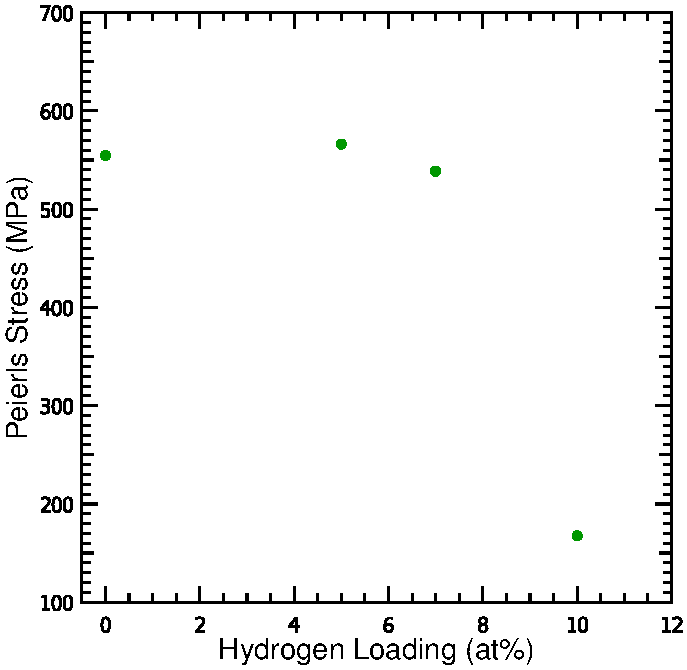
\includegraphics[width=0.5\textwidth]{Peierls_Stress_Cementite}
\caption[The effect of hydrogen on the Peierls stress of cementite]{The effect of hydrogen loading on the predicted Peierls stress of cementite on the [100](010) slip system.\label{fig:tp_cementite}}
\end{figure}


\FloatBarrier
\subsection{Dislocations in ionic solids}
\FloatBarrier


Energy changes in ionic solids were fitted with an empirical function in a similar manner to that described in section~\ref{sec:elastic_results} except now the energy components are not misalignment and strain energy terms but electrostatic and short-range terms. This was done for the two slip systems known to operate in crystals with the rocksalt structure, the <1\,1\,0>\{0\,0\,1\} and the <1\,1\,0>\{1\,\={1}\,0\}.


First the energy was calculated via a Python program, the code is available online \cite{code}, that used a simple approach: calculating the energy for all the interactions in the crystal with no cut offs. This gives the energy without the risk of artefacts that can be introduced by cut offs, but at the cost of computational time. Importantly the energy of the dislocation itself is difficult to estimate, since the energy calculated by this method includes the energy of the whole crystal, including the energy of the free surfaces and so on. This was addressed by assuming that the energy changes were due to the dislocation alone, which is reasonable because the faces of the dislocated crystal are far enough from the dislocation not to deform very much.


The energy changes calculated in this way, using the same optimisation procedure as described above, are shown in \autoref{fig:NaCl_energy_changes}. There is a curious result that the periodicity appears to be different for the two dislocations, a period of $b$ for the <1\,1\,0>\{1\,\={1}\,0\} slip system and $^b\!/_2$ for the <1\,1\,0>\{0\,0\,1\} slip system. This can be explained in terms of the crystal structure. 

Considering the core structures shown in \autoref{fig:Schematic_NaCl_dislocs}, for the <1\,1\,0>\{0\,0\,1\} slip system the $\alpha=0.5$ position is nearly equivalent to the $\alpha=0$ position. The two positions can be related by swapping all the cations for anions and vice versa. The result is that the electrostatic energy must be the same. Since the short range potential used here is symmetrical for anion-cation or cation-anion interactions, all the first neighbour interactions will also be the same since there are no cation-cation or anion-anion neighbours to swap. There will be differences in the second nearest neighbours, which change from anion-anion to cation-cation interactions and vice versa. This difference is observed; the halfway position is lower in energy than the initial position by \SI{1.4e-22}{\joule\per\meter}. This is a very small difference as expected, but is within the expected precision of the calculation. Thus strictly the period of the dislocation energy is $b$, but for practical purposes can be treated as $^b\!/_2$. Such a similarity does not exist for the <1\,1\,0>\{1\,\={1}\,0\} slip system, so the period is more plainly $b$ without extra minima.





\begin{figure}
\centering
\begin{subfigure}{0.4\textwidth}
\centering
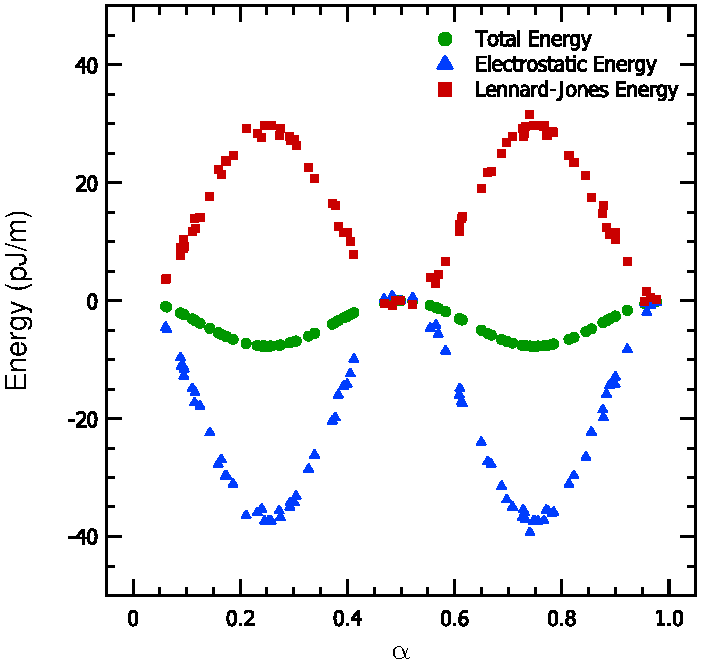
\includegraphics[width=\textwidth]{NaCl_110_001_U_vs_alpha}
\caption{The energy changes with displacement of a <110>\{001\} dislocation in NaCl.\label{fig:NaCl_110_001_energy_changes}}
\end{subfigure}
~
\begin{subfigure}{0.4\textwidth}
\centering
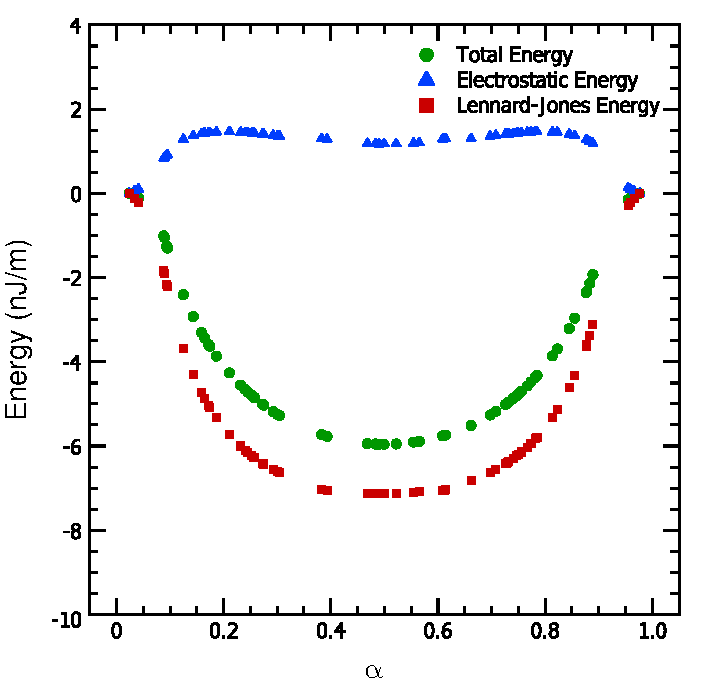
\includegraphics[width=\textwidth]{NaCl_110_110_U_vs_alpha}
\caption{The energy changes with displacement of a <110>\{1\={1}0\} dislocation in NaCl.\label{fig:NaCl_110_110_energy_changes}}
\end{subfigure}
\caption[The energy changes with position of dislocation in NaCl.]{The energy changes with position of dislocation in NaCl. Note that the scale of the energy changes is much larger for the <110>\{1\={1}0\} slip system.\label{fig:NaCl_energy_changes}}

\end{figure}



\begin{figure}
\centering
\begin{subfigure}{55mm}
\centering
\includegraphics[width=\textwidth]{zero}
\caption{}
\end{subfigure}
~
\begin{subfigure}{55mm}
\centering
\includegraphics[width=\textwidth]{half}
\caption{}
\end{subfigure}


\caption[The symmetrical positions of dislocations in NaCl.]{Dislocations in NaCl showing the similarity between the two symmetrical positions; if the short range potential were applied to only first neighbours these would be equivalent, related by reflection through the plane normal to the slip direction, in this case [1\,1\,0]. Graphics prepared with VESTA \cite{Momma2011}.\label{fig:NaCl_symmetry}}
\end{figure}


The data was fitted using the function given in \autoref{eqn:empirical_function}, and this gave the Peierls stress of the two systems as \SI{76.6}{\mega\pascal} for the <1\,1\,0>\{0\,0\,1\} slip system, and \SI{63.7}{\giga\pascal} for the <1\,1\,0>\{1\,\={1}\,0\} system. The value for <1\,1\,0>\{0\,0\,1\} system within a factor of 2 of experimental measurements of the Peierls stress, \citet{Haasen1985} estimated the Peierls stress of this slip system to be \SI{140}{\mega\pascal}. The value for the <1\,1\,0>\{1\,\={1}\,0\} slip system is clearly not in agreement with the estimated Peierls stress of \SI{10}{\mega\pascal}.



The variation of the dislocation width is shown in \autoref{fig:NaCl_w_vs_alpha}. The period of the variation of the width for the two slip systems is the same as that of the energy variation. The <1\,1\,0>\{0\,0\,1\} slip system shows the expected behaviour, small and smooth variation, \autoref{fig:NaCl_110_001_w_variation}, though there is some noise in the graph showing that perhaps the model has not fully converged on the lowest energy value. There is a much larger variation in the width for the <1\,1\,0>\{1\,\={1}\,0\} slip system, \autoref{fig:NaCl_110_110_w_variation}, and there is a discontinuity in the value at around $\alpha=0.1$. This corresponds to the very steep part of the energy variation shown in \autoref{fig:NaCl_110_110_energy_changes}.


\begin{figure}
\centering
\begin{subfigure}{0.4\textwidth}
\centering
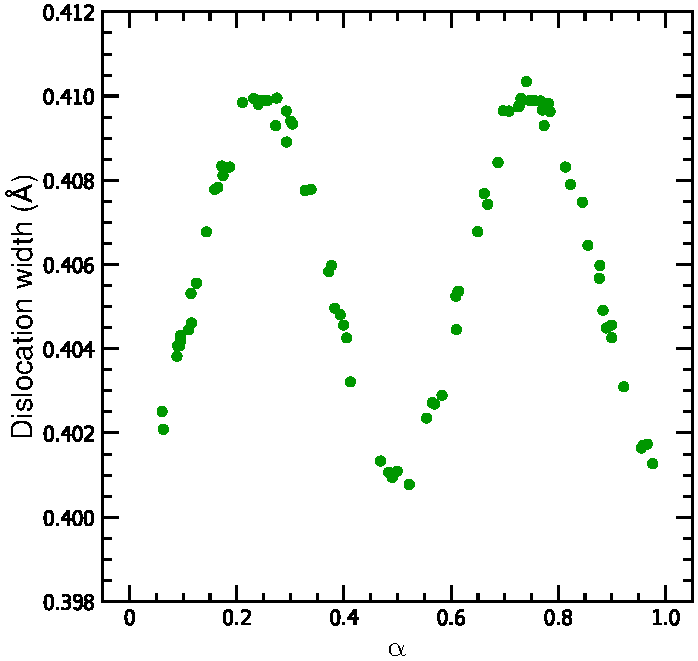
\includegraphics[width=\textwidth]{NaCl_110_001_w_vs_a}
\caption{The variation of the dislocation width with dislocation position for the <1\,1\,0>\{0\,0\,1\} slip system. \label{fig:NaCl_110_001_w_variation}}
\end{subfigure}
~
\begin{subfigure}{0.4\textwidth}
\centering
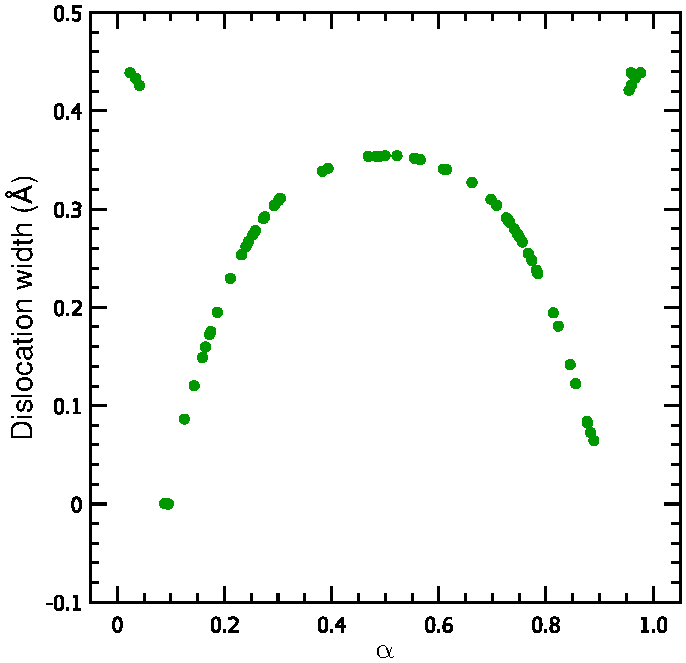
\includegraphics[width=\textwidth]{NaCl_110_110_w_vs_a}
\caption{The variation of the dislocation width with dislocation position for <1\,1\,0>\{1\,\={1}\,0\} slip system.\label{fig:NaCl_110_110_w_variation}}
\end{subfigure}
\caption[The variation of the dislocation width with position for NaCl.]{The variation of the dislocation width with position for the two slip systems of NaCl. The <1\,1\,0>\{0\,0\,1\} slip system shows the expected behaviour, showing relatively small variation in a smooth and continuous manner. The <1\,1\,0>\{1\,\={1}\,0\} slip system shows a much larger variation and a rapid if not discontinuous change at around $\alpha=0.1$.\label{fig:NaCl_w_vs_alpha}}
\end{figure}

One problem with modelling dislocations in ionic materials is the computational complexity compared to the elastic case. The model must be three dimensional since the interactions are three dimensional, which means the number of atoms is larger. Additionally the calculation scales more quickly with the size of the simulation, since now there are $n^2$ energy calculations to do for $n$ atoms rather than simply $n$ for the elastic energy calculation. Thus despite using the NumPy \citep{Numpy2011}, which is well optimised to efficiently undertake calculations, the scale of the simulation was much more limited, extending only tens of nanometers rather than hundreds from the dislocation core. Given the inherently long range nature of the electrostatic interaction this is potentially insufficient.

To address this, the model was adapted to use the LAMMPS \cite{LAMMPS_web} software package to undertake the energy calculation, using the Coulombic and Lennard-Jones calculators built in to the LAMMPS package. An example script and input files are included in \autoref{sec:lammps_input}. The principle is much the same, though now the energy calculation is using the highly optimised LAMMPS routines. These rely on choosing appropriate parameters and settings, which was done according to the LAMMPS manual \cite{LAMMPS_web}. One particular advantage is the ability to employ periodic boundary conditions along the length of the dislocation line, thus removing potential artefacts that might arise from the termination of the dislocation.

The results for the <1\,1\,0>\{1\,\={1}\,0\} slip system are shown in \autoref{fig:NaCl_110_110_U_vs_a_LAMMPS}. The variation is quite similar to that found using the na\"ive Python based energy calculator despite the periodic boundary conditions along the dislocation line and extending the simulation out from the core to \SI{\sim 100}{\nano\meter}. The maximum gradient of the best fit achievable using \autoref{eqn:empirical_function} gives the Peierls stress as \SI{63.8}{\giga\pascal}, which is very close to the the result obtained earlier, with an original calculator written in Python, as shown in \autoref{fig:NaCl_110_110_energy_changes}. 


\begin{figure}
\centering
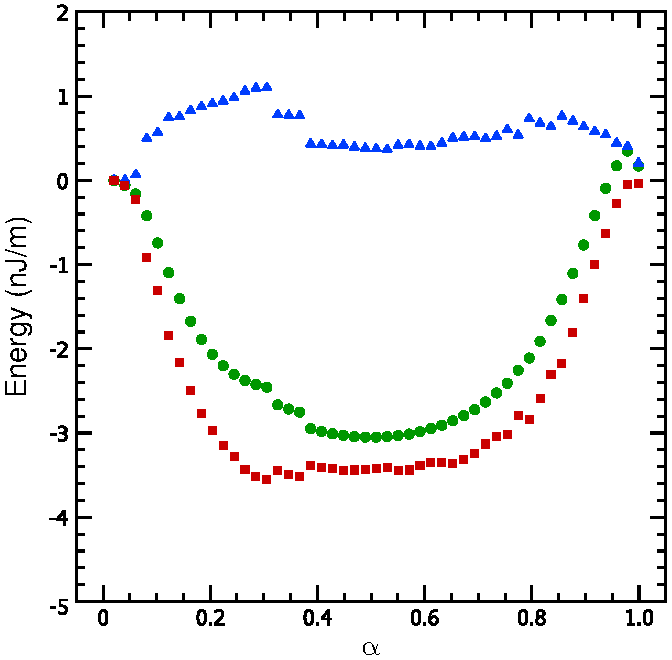
\includegraphics[width=0.5\textwidth]{NaCl_110_110_U_vs_alpha_LAMMPS}
\caption[The energy changes of a dislocation in NaCl via LAMMPS.]{The energy variation of a <1\,1\,0>\{1\,\={1}\,0\} dislocation in NaCl using the energy calculations available in LAMMPS. There is a lot of scatter, which does not appear to be random, but is likely due to insufficiently tight convergence criteria.\label{fig:NaCl_110_110_U_vs_a_LAMMPS}}
\end{figure}

The variation of the dislocation width with $\alpha$ is shown in \autoref{fig:LAMMPS_w_vs_a_NaCl}. There are some differences between the Python based model and the LAMMPS based model. Both models show a discontinuity in the width, dropping rapidly around $\alpha=0.1$, but the LAMMPS based model predicts zero width for $\alpha$ \numrange{\sim 0.1}{ 0.9}, where the Python based model predicted an increase to a maximum at $\alpha=0.5$. This might be attributable to the size of the simulation or the termination of the dislocation since those are the principle differences between the two models.

\begin{figure}
\centering
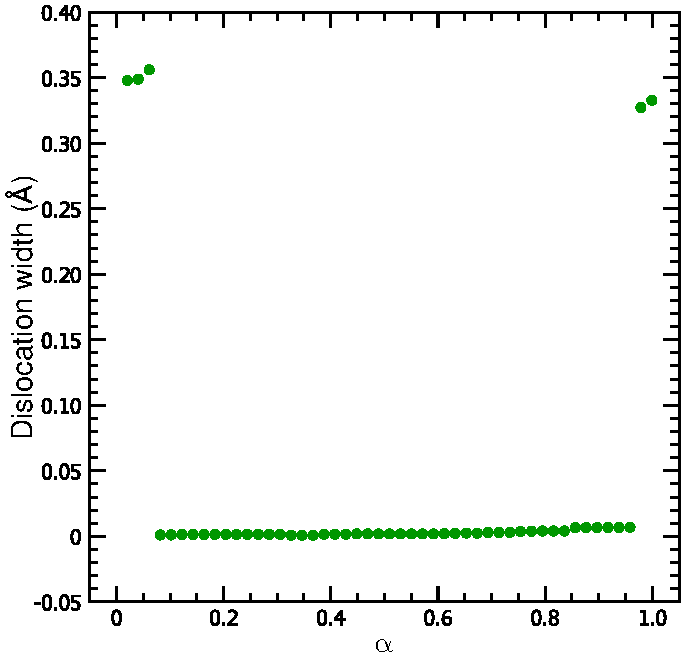
\includegraphics[width=0.5\textwidth]{NaCl_110_110_w_vs_a_LAMMPS}
\captionsetup{width=0.6\textwidth}
\caption[The variation of the dislocation width for the hard slip system in NaCl.]{The variation of the dislocation width with position for the <1\,1\,0>\{1\,\={1}\,0\} slip system in NaCl when using the energy as calculated by the LAMMPS software package.\label{fig:LAMMPS_w_vs_a_NaCl}}
\end{figure}


It therefore seems unlikely that simulation size or the termination of the dislocation at the free surface were major problems, instead some other factor is at fault. It is possible that core reconstruction occurs in NaCl such that the displacement field, \autoref{eqn:displacement_field}, is no longer appropriate. Other energetic considerations which have been neglected could be important, for example the polarisability of atoms has not been modelled. There are net dipoles around the <1\,1\,0>\{1\,\={1}\,0\} dislocation in NaCl but not around <1\,1\,0>\{0\,0\,1\} dislocations, which could explain the discrepancy. Since the Peierls model only deals in relatively small changes of a large value small factors such as this can be important.


\section{Conclusions}

A parametrised form of the displacement field around an edge dislocation has been reached by adapting the solution for an isotropic elastic medium. This allows the construction of atomic configurations in three dimensions rather than one. This formulation also reduces the parameter space that must be searched for the optimal dislocation structure to a tractable size.

A series of Python modules have been written to allow the modelling of dislocations in a variety of materials using a variational approach to minimise the energy of the atomic configuration for every dislocation position. The Peierls stress is calculated from the maximum gradient of the dislocation energy. The modular nature allows functionality to be added or altered easily. 

The first module builds the dislocation by constructing an array representation of atomic coordinates around the dislocation core via the adapted displacement field. This is deliberately left extensible to allow, for example, the addition of a screw dislocation or core reconstruction.

Two further modules have been written to calculate the energy of a dislocation as represented by an array of atomic coordinates. One builds on the existing Peierls models that use linear elasticity for strain energies away from the slip plane and a misalignment potential for the slip plane, either approximated as a sinusoid that obeys Hooke's law at low strains, or fitted empirically to \emph{ab initio} calculations of the $\gamma$-surface. This module extends the Peierls analysis to use the full stiffness tensor rather than simple elastic constants. The other uses the electrostatic interaction and the Lennard-Jones potential to calculate the energy of a dislocation in an ionic solid.

The elastic Peierls model is in agreement with the trends in material behaviour observed in experiment and predicted by previous models. However the effect of lattice geometry is not as strong in this model as is observed by experiment, consistent with previous models that have a periodicity of a full, rather than a half,  Burgers vector, thus only qualitative conclusions can be drawn. The model does predict a softening of the cementite structure when hydrogen is added, as predicted by experiment.

The ionic Peierls model successfully predicts the behaviour of the <1\,1\,0>\{0\,0\,1\} slip system in \ce{NaCl} as observed by experiment. The electrostatic and short-range repulsion energy components vary out of phase with each other, in a parallel to the strain energy and misalignment energy in traditional Peierls models. The behaviour of the <1\,1\,0>\{1\,\={1}\,0\} slip system is not successfully predicted. It was shown that this was not due to the size of the simulation or the termination of the dislocation line at a free surface by the use of LAMMPS as an energy calculator, which allowed much larger simulations and the use of periodic boundary conditions. Other explanations are the lack of polarisability in the atom potentials used or the possibility of dislocation core reconstruction, which were not treated by the model.






















\cleardoublepage

% The case for elastic heterogeneity in layered crystals
\chapter{Heterogeneity in the MAX phases}
\label{chap:hetero_max_phases}

\graphicspath{{hetero_max_phases/Figs/}}


As  discussed in \autoref{sec:ductility_criteria} the MAX phases are predicted to be brittle by a wide range of ductility criteria but they are in fact observed to be damage tolerant and to flow easily in the basal plane \cite{Barsoum1999}.
Predictions of the Peierls stress made using the methods described in \autoref{sec:dislocations} have been made previously \cite{Music2007ductility,Gouriet2015}, however these have had limited success, producing over estimates, for example \citet{Gouriet2015} reported the Peierls stress to be at least \SI{611}{\mega\pascal} which is similar to  that estimated for titanium carbide and other very hard brittle materials in which slip is limited at room temperature by the Peierls mechanism \cite{Chang1966,Clegg2006,Kamimura2011,Yadav2014}. Given that flow stresses in the region of a few tens of \si{\mega\pascal} have been observed at room temperature \cite{Humphrey2012,Barsoum1999}, which is more comparable with FCC metals than FCC carbides, it is reasonable to expect the Peierls stress of MAX phases to be lower than that of TiC.

The poor performance of Peierls models for MAX phases, and potentially for other complex phases, might be due to the treatment of the MAX phase unit cell as elastically homogeneous. This is surprising because many studies have discussed the heterogeneity of the bonding and electron structure, one recent review was written by \citet{Magnuson2017}, and discusses the complex and mixed nature of the bonding varying across the different atomic sites, more metallic in the MA layers, more covalent in the MX layers, and charge transfer contributing an ionic component to the bonding. 

The bonding is associated with many of properties of the MAX phases, for example high melting point, high specific stiffness, electrical and thermal conductivity, and a near zero Seebeck coefficient to name a few \cite{Yoo2000,Sun2011,Magnuson2017} but the clear and strong heterogeneity of the unit cell has largely been neglected when considering the mechanical properties of the MAX phases, the only consideration of the atomic environments  being the choice of plane at which the generalised stacking fault energy was calculated \cite{Music2007ductility}.


\section{Chemical heterogeneity}

Measuring single crystal elastic constants for the MAX phases is extremely difficult due to the difficulty of growing single crystals and experimentally determining the stiffness of sub-unit cell regions of the crystal presents an even greater challenge. Instead density functional theory can be employed. DFT has been widely used to calculate single crystal elastic constants of a large variety of materials and is considered reliable and reproducible \cite{Lejaeghere2016}. 



If the MAX phases are elastically heterogeneous there is the question of what might be the expected properties and how these might vary within the MAX phase unit cell. A simple way of characterising the chemical heterogeneity is the electronegativity, $\chi$, of regions within the unit cell. For both the M--X and M--A regions, an average electronegativity is easily calculated as once sharing of atoms between the regions is accounted for there are equal numbers of M and A atoms in the M--A region and similarly equal numbers of M and X atoms in the M--X region. The difference in electronegativity between the two regions is therefore defined by
\begin{equation}
\Delta \chi = \frac{\chi_{\text{X}} - \chi_{\text{A}}}{2}\label{eqn:MAX_electronegativity_diff}
\end{equation}
since the M atoms contribute to both regions. 

There are a variety of measures of electronegativity, but perhaps the most fundamental and transferable is the Mulliken scale \cite{Mulliken1934}, which takes the electronegativity of a species to be the average of the ionization energy, the energy change upon removing an electron, and the electron affinity, the energy change upon adding an electron. This scale is more fundamental than others because it is calculated from the fundamental properties of atoms, as opposed to more ``relative'' scales that are calculated from enthalpies of formation and covalent radii and so on \cite{huheey1983ch3_electronegativity}.

Since the elements that take the X site, carbon and nitrogen, are generally more electronegative than those that take the A site, elements like aluminium and silicon, it is expected that electron transfer into the M--X region from the M--A \cite{Sun2011}. Such a transfer would be expected to increase the strength of the bonding in the M--X layer and reduce it in the M--A, with a corresponding change in the moduli of the two regions.


\section{Density functional theory calculations}
\label{sec:DFT_method}



Measuring single crystal elastic constants for the MAX phases is extremely challenging due to the difficulty of growing single crystals and experimentally determining the stiffness of sub-unit cell regions of the crystal presents an even greater challenge. Instead density functional theory can be employed. DFT has been widely used to calculate single crystal elastic constants of a large variety of materials and is considered reliable and reproducible \cite{Lejaeghere2016}. 

%%% Better check I've referenced this correctly and that I understand it enough
The density functional theory calculations were performed with the SIESTA package \cite{soler2002}, a pseudopotential based LCAO package using semicore pseudopotentials with partial core corrections in the Perdew-Burke-Ernzhof (PBE) formulation generated and tested by the ATOM implementation \cite{soler2002} of the Troullier-Martins procedure \cite{Troullier1991,Troullier1991a} as described in the software documentation \cite{ATOM_manual}. A double-$\zeta$ polarised basis set including the semicore states was used, the cutoff radii of which were optimised with a variational simplex method.

The starting point for the calculations presented here were a series of optimised unit cells for a range of MAX phases produced by a procedure developed by Philip Howie. A optimisation approach to generating suitable pseudopetentials was taken using ATOM \cite{ATOM_manual}; pseudopotentials with a range of cut off radii were tested against all-electron calculations of the atomic ground state and a number of excited states and the cut off radius is improved until the best (i.e. closest to all-electron) pseudopotential is identified. 

Firstly some simulation parameters have to be optimised, the k-grid size and the mesh cut off. Suitable values are chosen to provide sufficient accuracy and ensure the energy converges \cite{SIESTA_manual}.

Once pseudopotentials and the simulation parameters have been generated the lattice parameters are optimised. The literature values are used as the starting point but the calculated equilibrium lattice parameter is typically \SIrange{1}{2}{\percent} bigger that the experimental value when using the generalised gradient approximation \cite{Staroverov2004,Wu2006}. Initially the lattice parameter ratio, $c/a$, is kept fixed and the lattice parameter $a$ is varied to reduce the hydrostatic pressure to zero.

The basis set was optimised with this roughly equilibrated unit cell. Most of the variables are taken to be suggested values  from examples provided by the authors of SIESTA \cite{SIESTA_manual}. The problem is variational, i.e. a lower energy means a better basis set; so the basis set is optimised by the simplex optimisation method, also known as the Nelder-Mead method \citep{Nelder1965}.

With an accurate basis set the lattice parameters are now optimised to find the true equilibrium point, relaxing both $a$ and $c$ to reduce the stresses to zero (or equivalently finding the minimum energy).


Many of the atomic positions are fixed by symmetry, but those parameters that are free to vary without breaking the structure's symmetry are relaxed. These are the heights in the $c$-axis of some of the atoms as shown in \autoref{fig:MAX_unit_cells}.


A comparison of the lattice parameters generated by DFT with Howie's method is shown in \autoref{fig:unit_cells_DFT_vs_literature} and the data are summarised in \autoref{tab:MAX_DFT_unit_cell_results}. The agreement is good as expected, particularly in the lattice geometry, $c/a$. The better agreement in $c/a$ than in the lattice parameters themselves is because the errors inm the lattice parameters are correlated, so that both $a$ and $c$ are in error (usually too large) by the same fraction. These equilibrated unit cells were used as the basis for further investigation of MAX phase behaviour.

\begin{figure}
\begin{subfigure}{\textwidth}

\centering
\captionsetup{width=10cm}
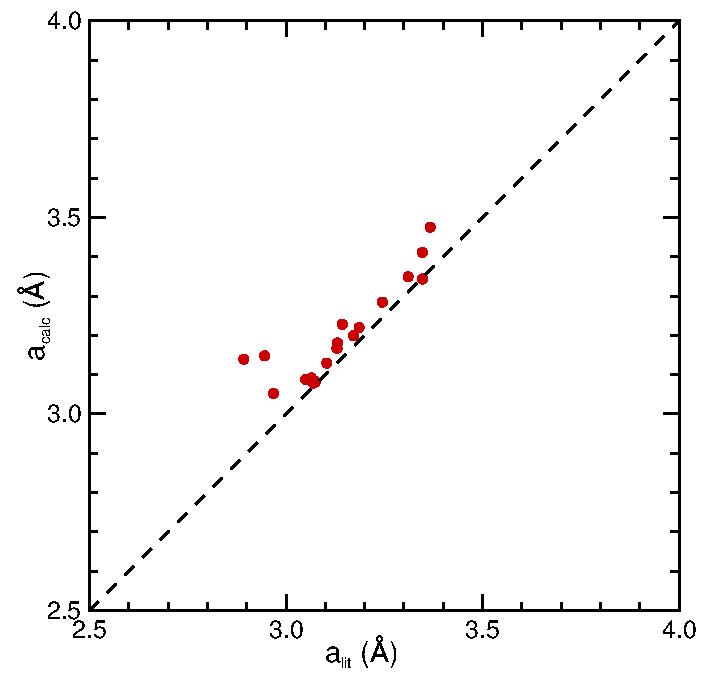
\includegraphics[width=8cm]{a_calc_vs_a_lit}
\caption[Calculated lattice parameters compared with literature values]{A comparison between the lattice parameter, $a$, calculated here with literature values.\label{fig:latt_params_DFT_vs_lit}}

\end{subfigure}

\begin{subfigure}{\textwidth}
\centering
\captionsetup{width=10cm}
\includegraphics[width=8cm]{c-a_calc_vs_lit}
\caption{A comparison between the calculated lattice parameter ratio, $c/a$, with literature values.\label{fig:c_a_ratio_DFT_vs_lit}}
\end{subfigure}

\caption[A comparison of the unit cells calculated by DFT with the literature.]{A comparison of the unit cells calculated by DFT with those reported in the literature. There is reasonable agreement between the lattice parameters $a$ calculated here and found experimentally in the literature. The lattice geometry, $c/a$, is in excellent agreement with reported values.\label{fig:unit_cells_DFT_vs_literature}}
\end{figure}



\begin{sidewaystable}
\begin{tabular}{|l|c|c|c|c|c|c|c|c|c|c|c|c|c|c|}
\hline
Phase &       $a$ &     $a_{\text{lit}}$ &     $c/a$ & $c/a_{\text{lit}}$ &       $z_1$ &    $z_{1,\text{lit}}$ &       $z_2$ &   $z_{2,\text{lit}}$ &      $z_3$ &    $z_{3,\text{lit}}$ &       $d/b$ &     $z_{\text{M--A}}$ &      $d_{\text{M--A}}$ \\
\hline
   \ce{Nb2AlC}\rule[3ex]{0pt}{0pt} &  3.1297 &  3.1035 &  4.5215 &  4.5213 &  0.0898 &  0.0880 &       - &       - &       - &       - &  0.7243 &  0.1602 &  2.2479 \\
   \ce{Nb2GaC}                     &  3.1806 &  3.1310 &  4.3322 &  4.3325 &  0.0887 &  0.0880 &       - &       - &       - &       - &  0.6988 &  0.1613 &  2.1880 \\
   \ce{Nb2InC}                     &  3.1987 &  3.1720 &  4.5303 &  4.5303 &  0.0827 &  0.0860 &       - &       - &       - &       - &  0.7579 &  0.1673 &  2.4041 \\
    \ce{Nb2SC}                     &  3.3484 &  3.3100 &  3.4862 &  3.4864 &  0.0944 &  0.0990 &       - &       - &       - &       - &  0.5425 &  0.1556 &  1.7956 \\
   \ce{Nb2SnC}                     &  3.2844 &  3.2450 &  4.2441 &  4.2435 &  0.0833 &  0.0850 &       - &       - &       - &       - &  0.7074 &  0.1667 &  2.2954 \\
   \ce{Ti2AlC}                     &  3.0517 &  2.9680 &  4.5422 &  4.4554 &  0.0844 &  0.0882 &       - &       - &       - &       - &  0.7378 &  0.1656 &  2.1898 \\
   \ce{Ti2GaC}                     &  3.0914 &  3.0640 &  4.3431 &  4.3424 &  0.0855 &  0.0880 &       - &       - &       - &       - &  0.7143 &  0.1645 &  2.1887 \\
   \ce{Ti2InC}                     &  3.1481 &  2.9450 &  4.4905 &  4.4852 &  0.0790 &  0.0829 &       - &       - &       - &       - &  0.7670 &  0.1710 &  2.2587 \\
    \ce{Ti2SC}                     &  3.2279 &  3.1432 &  3.5172 &  3.5158 &  0.0977 &  0.0998 &       - &       - &       - &       - &  0.5355 &  0.1523 &  1.6830 \\
   \ce{Ti2SnC}                     &  3.2196 &  3.1860 &  4.2786 &  4.2781 &  0.0807 &  0.0790 &       - &       - &       - &       - &  0.7243 &  0.1693 &  2.3076 \\
   \ce{Zr2InC}                     &  3.3434 &  3.3470 &  4.4541 &  4.4547 &  0.0874 &  0.0860 &       - &       - &       - &       - &  0.7243 &  0.1626 &  2.4243 \\
    \ce{Zr2SC}                     &  3.4755 &  3.3663 &  3.5711 &  3.5714 &  0.0998 &  0.1013 &       - &       - &       - &       - &  0.5364 &  0.1502 &  1.8058 \\
   \ce{Zr2SnC}                     &  3.4110 &  3.3470 &  4.3590 &  4.3591 &  0.0854 &  0.0860 &       - &       - &       - &       - &  0.7175 &  0.1646 &  2.4015 \\
  \ce{Ti3AlC2}                     &  3.0831 &  3.0730 &  6.0390 &  6.0387 &  0.0710 &  0.0691 &  0.1305 &  0.1276 &       - &       - &  0.7216 &  0.1224 &  2.2714 \\
  \ce{Ti3SiC2}                     &  3.0820 &  3.0747 &  5.7642 &  5.7620 &  0.0727 &  0.0722 &  0.1355 &  0.1353 &       - &       - &  0.6600 &  0.1147 &  2.0321 \\
  \ce{Nb4AlC3}                     &  3.1674 &  3.1296 &  7.7081 &  7.7073 &  0.0549 &  0.0552 &  0.1088 &  0.1086 &  0.1575 &  0.1574 &  0.7130 &  0.0926 &  2.2345 \\
  \ce{Ti4GaC3}                     &  3.0781 &  3.0690 &  7.6371 &  7.6377 &  0.0516 &  0.0558 &  0.1091 &  0.1068 &  0.1549 &  0.1564 &  0.7263 &  0.0936 &  2.1940 \\
 \ce{Ti4SiC3}\rule[-1ex]{0pt}{0pt} &  3.0878 &  3.0500 &  7.3627 &  7.3614 &  0.0535 &  0.0532 &  0.1120 &  0.1118 &  0.1603 &  0.1599 &  0.6604 &  0.0901 &  2.0230 \\
\hline
\end{tabular}
\caption{The unit cell parameters as modelled by density functional theory and some literature values for comparison.\label{tab:MAX_DFT_unit_cell_results}}
\end{sidewaystable}

\section{Calculating the local stiffness}


One method for calculating the elastic constants via DFT is simply to simulate the unit cell with periodic boundary conditions and apply a stress/strain state and fit either the equation
\begin{equation}
\sigma_{ij} = C_{ijkl} \epsilon_{kl}
\end{equation}
or 
\begin{equation}
u = \frac{1}{2} C_{ijkl} \epsilon_{ij} \epsilon_{kl}
\end{equation}
where $\sigma_{ij}$ is the stress tensor, $\epsilon_{ij}$ is the strain tensor, $u$ is the strain energy per unit volume and $C_{ijkl}$ is the stiffness tensor. This was applied by \citet{Aryal2014} to a very wide range of MAX phases. Care must be taken to reproduce the physically realistic situation where the stress is equal throughout the unit cell but the strain can vary, i.e. the strain must be applied macroscopically to whole the simulation cell but the atomic positions must then be allowed to relax into the lowest energy configuration.

The latter equation was used to find the local stiffness within a region of the unit cell. The single crystal elastic constants must be dropped since a tensor formulation of heterogeneous elasticity is not the aim, instead local shear moduli are calculated. The unit cell is divided naturally into two distinct regions that are obvious from the geometry of the crystal structure, the local chemistry and nature of bonding, there is a more metallic layer, the M--A layer, and a more covalent layer, the M--X layer, see \autoref{fig:MAX_unit_cells}. The layer of M-atoms that are bonded to both A-atoms and X-atoms is the natural boundary.

To localise the strain in, say, the M--A layer all the bonding, that is the relative atomic positions, in the M--X layer are held rigid and are displaced as a whole such that in each M--A layer the appropriate strain is applied. The relative positions of the atoms within the M--A layer are then allowed to relax to achieve the minimum energy. The equation that must then be fitted is
\begin{equation}
u = \frac{1}{2} G_{i} \gamma^2
\end{equation}
where $\gamma$ is the applied strain and $G_i$ is the local shear modulus, namely either $G_{M\text{--}A}$ or $G_{M\text{--}X}$. The procedure is applied vice versa to calculate the M--X properties.




\begin{figure}
\centering
\captionsetup{width=0.5\textwidth,font={sf,scriptsize},labelfont=bf}
\includegraphics[height=0.3\textheight]{slab_model}
\caption[Hetergeneous strain in a sheared MAX phase unit cell.]{Schematic of non-uniform elastic deformation in a ``211'' MAX phase showing the regions that might be considered distinct, the M--A and M--X layers.\label{fig:slab_model}}
\end{figure}


\captionsetup{width=\textwidth,font={sf,scriptsize},labelfont=bf}


The overall shear modulus for the whole crystal structure is calculated in the same manner with no restrictions on the atomic positions, all the atoms are allowed to relax fully. Since this relaxed shear is equivalent to a uniform applied stress an analogy is possible with the assumptions made to calculate the transverse stiffness of long fibre composite materials, the so called slab model \cite{Hull1996ch4}. The slab model is illustrated in \autoref{fig:slab_model}. The results of the local calculations can be compared with the overall case using the equation:
\begin{equation}
G_{\text{slab}} = \left[ \frac{f_{M\text{--}X}}{G_{M\text{--}X}} + \frac{f_{M\text{--}A}}{G_{M\text{--}A}} \right]^{-1} \label{eqn:slab_model}
\end{equation}
where $G_{\text{slab}}$ is the estimate for the overall shear modulus, $f_i$ is the volume fraction of the region $i$ and $G_i$ is the shear modulus of region $i$. The volume fractions are estimated from the crystal structures of the MAX phases. In particular the fractional coordinate in the $c$ direction of the M1 site in the 211 phases, $z_1$, and the position of the M2 site in the 312 and 413 phases, $z_2$, as shown in \autoref{fig:MAX_unit_cells}, determines the volume fraction of the regions of the unit cell:

\begin{subequations}
\begin{align}
f_{\text{M--A}} &= 
\begin{cases}
1-4z_1 & \qquad \text{for 211 phases} \\
4z_2 & \qquad \text{for 312 and 413 phases}
\end{cases}  \\[1ex]
f_{\text{M--X}} &= 
\begin{cases}
4z_1 & \qquad \text{for 211 phases} \\
1 - 4z_2 & \qquad \text{for 312 and 413 phases}
\end{cases}
\end{align}
\end{subequations}

\section{Results and Discussion}

The moduli of the separate layers are presented in \autoref{fig:Gma_variation} and summarised in \autoref{tab:MAX_DFT_elastic_results}. The M--X layer is stiffer than the M--A layer for all the MAX phases studied here, as expected from the nature of the bonding in the MAX phases as discussed in \autoref{sec:layered_crystals}. There is an overall increase in the stiffness of the M--X layer and an overall decrease in the stiffness of the M--A layer as the electronegativity difference between these layers increases, although the data is scattered around that correlation, presumably as more complex chemical factors operate in addition to electronegativity differences.


The trend is clearer when the ratio of the moduli is considered, as shown in \autoref{fig:ratio_of_Gma_to_Gmx}. The ratio $G_{\text{M--A}}/G_{\text{M--X}}$ varies with the electronegativity difference between the layers, so even where other chemical effects cause the overall bonding to be stronger the \emph{relative} moduli of the two layers are altered by electrons being drawn from the M--A layer into the M--X layer to varying extents. In the case of A atoms like indium or gallium electrons are easily lost from the M--A layer to the M--X layer, reducing the ratio, while in the case of sulphur occupying the A site there is almost no electronegativity difference between the layers and the ratio is higher.


\begin{figure}
\centering

\begin{subfigure}{0.4\textwidth}
\centering
\captionsetup{font={sf,scriptsize},labelfont=bf}
\includegraphics[width=\textwidth]{Gmx_and_Gma_dX_MAX}
\caption{The variation of shear moduli of the M--A and the M--X layers.  \label{fig:Gma_variation}}
\end{subfigure}
~
\begin{subfigure}{0.4\textwidth}
\centering
\captionsetup{font={sf,scriptsize},labelfont=bf}
\includegraphics[width=\textwidth]{Gma_Gmx_vs_dX}
\caption{The variation of the ratio of the shear moduli of the M--A and the M--X layers. \label{fig:ratio_of_Gma_to_Gmx}}
\end{subfigure}

\begin{subfigure}{0.4\textwidth}
\centering
\captionsetup{font={sf,scriptsize},labelfont=bf}
\includegraphics[width=\textwidth]{dma_vs_dX}
\caption{The variation of the M--A bond length. \label{fig:bond_length}}
\end{subfigure}
~
\begin{subfigure}{0.4\textwidth}
\centering
\captionsetup{font={sf,scriptsize},labelfont=bf}
\includegraphics[width=\textwidth]{Grel_vs_dX}
\caption{The variation of the overall shear modulus, $G_{\text{rel}}$. \label{fig:overall_G_vs_dX}}
\end{subfigure}

\begin{subfigure}{\textwidth}
\centering
\captionsetup{width=0.6\textwidth,font={sf,scriptsize},labelfont=bf}
\includegraphics[width=0.4\textwidth]{Gslab_vs_Grel}
\caption{A comparison of the overall shear modulus of the MAX phases, $G_{\text{rel}}$, and the shear modulus calculated from the local shear moduli using the slab model, $G_{\text{slab}}$. The dotted line is $y=x$. \label{fig:Gslab_vs_Grel}}
\end{subfigure}

\caption[The local elastic properties of the MAX phases.]{The results of modelling by DFT the elastic properties of the MAX phases. $\Delta \chi$ is the electronegativity difference between the M--A and M--X layers. Circles, squares and triangles represent 211, 312, and 413 phases respectively.}

\end{figure}

\begin{table}
\centering
\begin{tabular}{|l|c|c|c|c|c|c|}
\hline
Phase \rule[3ex]{0pt}{0pt} &  $G_{\text{rel}}$ &     $G_{\text{M--A}}$ &    $G_{\text{M--X}}$ &  $G_\text{slab}$ &  $G_{\text{M--A}}/G_{\text{M--X}}$ &  $\Delta \chi$ \\
\hline
\ce{Nb2AlC} \rule[3ex]{0pt}{0pt}   &     137.7 &  101.9 &  230.4 &  127.4 &      0.442 &   1.5260 \\
\ce{Nb2GaC}                        &     113.4 &   79.1 &  236.6 &  103.6 &      0.334 &   1.5233 \\
\ce{Nb2In}                         &     112.2 &   82.3 &  251.6 &  105.9 &      0.327 &   1.5880 \\
\ce{Nb2SC}                         &     141.8 &  103.9 &  225.1 &  130.4 &      0.462 &   0.0214 \\
\ce{Nb2SnC}                        &     107.4 &   81.2 &  229.5 &  103.5 &      0.354 &   1.0166 \\
\ce{Ti2AlC}                        &     123.0 &   89.3 &  289.5 &  116.5 &      0.308 &   1.5260 \\
\ce{Ti2GaC}                        &     107.0 &   77.0 &  262.2 &  101.5 &      0.294 &   1.5233 \\
\ce{Ti2InC}                        &      95.5 &   71.4 &  248.0 &   92.1 &      0.288 &   1.5880 \\
\ce{Ti2SC}                         &     169.8 &  129.3 &  220.8 &  154.3 &      0.586 &   0.0214 \\
\ce{Ti2SnC}                        &      98.8 &   78.6 &  200.2 &   97.8 &      0.393 &   1.0166 \\
\ce{Zr2InC}                        &      75.4 &   48.1 &  209.3 &   65.8 &      0.230 &   1.5880 \\
\ce{Zr2SC}                         &     140.3 &   89.7 &  225.4 &  118.1 &      0.398 &   0.0214 \\
\ce{Zr2SnC}                        &      88.2 &   59.5 &  179.1 &   77.1 &      0.332 &   1.0166 \\
\ce{Ti3AlC2}                       &     129.1 &   83.3 &  230.9 &  101.8 &      0.361 &   1.5260 \\
\ce{Ti3SiC2}                       &     165.9 &  102.5 &  241.0 &  144.5 &      0.425 &   0.7453 \\
\ce{Nb4AlC3}                       &     167.6 &   95.8 &  262.2 &  159.5 &      0.365 &   1.2117 \\
\ce{Ti4SiC3} \rule[-1ex]{0pt}{0pt} &     161.4 &   84.3 &  215.6 &  138.1 &      0.391 &   0.7453 \\
\hline
\end{tabular}


\caption[Summary of the elastic properties calculated by density functional theory calculations.]{Summary of the elastic properties calculated by density functional theory calculations.\label{tab:MAX_DFT_elastic_results}}
\end{table}

This change is reflected in the bond lengths in the M--A layers, the bonds getting longer as electronegativity increases. This reflects a weakening of the bonds in the M--A layer as electrons are removed to the M--X layer.




The overall shear modulus was calculated in the same manner and also shows some variation with the electronegativity difference. The overall modulus is calculated by imposing an overall strain the unit cell and allowing the atomic positions to relax, hence this is termed the relaxed modulus, $G_{\text{rel}}$. There is an overall decrease in the shear modulus of the MAX phases as the electronegativity difference across the structure increases, the contribution of the weakening M--A bond lowering the overall shear modulus more than the strengthening of the M--X bonding raises it.


The slab model was used to compare the local moduli, $G_{\text{M--A}}$ and $G_{\text{M--X}}$,  with the overall modulus, $G_{\text{rel}}$, using \autoref{eqn:slab_model}. The results are plotted in \autoref{fig:Gslab_vs_Grel}. The correlation is very good, showing that the local properties are in agreement with the macroscopic properties.

\captionsetup{font={sf,scriptsize},labelfont=bf}


\section{Conclusions}

The MAX phases have been modelled with density functional theory calculations. The unit cells were optimised and found to be in good agreement with the literature. These unit cells formed the basis of further investigation.

The shear modulus of the M--A and M--X regions of the structure were investigated as well as that of the entire MAX phase structure. The shear modulus was calculated by examining the energy changes for a range of applied shear strains up to \SI{2}{\percent} and fitting to Hooke's law.

The shear moduli of both the M--A layer and the M--X layer varied with the electronegativity difference between them, as the difference increased (M--X becoming more electronegative) the M--A layer became more compliant and the M--X layer became stiffer. In particular the ratio of these moduli was well correlated with the electronegativity difference between the M--X and M--A layers.

The moduli of these regions of the unit cell were combined with the slab model to estimate the overall shear modulus, which matched well with DFT simulations of strains applied to the whole unit cell.






























\cleardoublepage
% The dislocations in MAX phases

\chapter{Dislocations in MAX phases}

\label{chap:dislocations_in_max_phases}
\graphicspath{{dislocations_in_max_phases/Figs/}}






In \autoref{chap:hetero_max_phases} elastic heterogeneity of the unit cell was discussed and the local elastic properties were shown to have a strong dependence on the chemical environment. As discussed in  \autoref{chap:plastic_deformation} and shown in \autoref{chap:peierls_model} the Peierls stress, i.e. the lattice resistance at \SI{0}{\kelvin}, is very sensitive to the elastic properties of a crystal. Thus the elastic heterogeneity is expected to have a strong effect on the dislocations in the MAX phases.

The elastic properties of the different layers of the MAX phases are not in the form of full elastic tensors so the approach taken in \autoref{chap:peierls_model} to use the full strain state cannot be applied. Instead a simplified model, adapted from that presented by \citet{Clegg2006} is used that relies on only simple strains and elastic constants. This model was shown to be in good agreement with experiment across orders of magnitude of the Peierls stress for a wide range of materials and is used here to demonstrate the effects of elastic heterogeneity on the Peierls stress.


\section{Adapted Peierls model}

The lack of a full elastic tensor means that the Peierls model used in this case was adapted from the one published by \cite{Clegg2006}. This works in a similar way to the model described in \autoref{chap:peierls_model} except only the first layer of atoms either side of the slip plane are considered and the only displacements allowed are parallel to the Burgers vector, in analogy with the original Peierls model.

The calculation essentially the same; the energy is still a balance between two energy contributions, the elastic energy in the bonds outside the slip plane and the misalignment energy of those bonds across the slip plane. The Peierls stress is then the maximum gradient of the energy changes as the dislocation is displaced. However some aspects are different.


The original model was written to calculate the misalignment energy using the Frenkel approximation, as given in \autoref{eqn:Frenkel_approx}, but the adapted model was extended to use a parametrised $\gamma$-surface to represent the misalignment energies, as represented by the summation
\begin{equation}
\gamma = \sum_{m=1}^{M} C_m \left[ 1 - \cos \left( \frac{2m\pi \phi}{b} \right) \right]\label{eqn:gamma_surface}
\end{equation}
where $\gamma$ is the energy in \si{\joule\per\meter\squared}, $C_m$ are a series of parameters fitted by a least-squares method to a set of energies at different misalignments, $m$ is an integer between 1 and some maximum $M$ which is chosen to be the lowest number that adequately captures the energy profile of the $\gamma$-surface, $b$ is the burgers vector and $\phi$ is the misalignment in units of \si{\angstrom}, such that $\phi/b$ defines a sort of fractional misalignment. It was generally found that $M=3$ was sufficient to capture the shape of the $\gamma$-surface, but was sometimes extended to six.

The other major difference is that the model in \cite{Clegg2006} optimises the structure of the dislocation only at the equilibrium position, not at every sampled displacement. The adapted model optimises the structure of the dislocation for every position by searching for the dislocation width that yields the lowest dislocation energy.


The elastic moduli and unit cell geometries, both required for the Peierls model, of the regions of the MAX phase structures have been calculated in \autoref{chap:hetero_max_phases} so the only other required input for the model is the misalignment potential, derived from the $\gamma$-surface.

\section{Calculating the \texorpdfstring{$\gamma$}{gamma}-surface}


The density functional theory used the same initial set-up as discussed in \autoref{sec:DFT_method}, based on the equilibrated unit cells with periodic boundary conditions in all directions. To calculate the gamma surfaces a displacement across a plane must be imposed, the simplest way to do this is to maintain the periodic boundary conditions and introduce two opposing stacking faults, this is shown schematically in \autoref{fig:DFT_gamma_surface}. There will be a dependence of the stacking fault energy on the distance between stacking faults, and this must be converged, in practice the lattice parameter of the MAX phases is long enough that only one or two unit cell repeats were necessary.

\begin{figure}
\centering
\captionsetup{width=0.45\textwidth}
\includegraphics[width=0.3333\textwidth]{displacements_for_gamma_surface}
\caption[Schematic displacements during the simulation of the \texorpdfstring{$\gamma$}{gamma}-surface.]{Schematic showing the displacements applied to a slab of crystal within a periodic cell to create two opposing stacking faults and find the energy changes, which will be twice the $\gamma$-surface. \label{fig:DFT_gamma_surface}}
\end{figure}

To displace the atoms SIESTA's Z-matrix was used \cite{SIESTA_manual}. This allows the coordinates of the atoms to be constrained separately in each direction; the displacement parallel to the slip direction, $a/3$<1\,1\,\={2}\,0> was imposed and the atomic positions were relaxed perpendicular to this displacement. This is important as unreasonably close atomic positions would occur without this relaxation. In analogy with the FCC metals it might be expected for there to be a stable stacking fault. The M--A layer can be seen as a single repeat of the HCP structure, with ABA stacking, which their stacking relative to the other M--A layer in the unit cell which is then stacked CBC, see \autoref{fig:MAX_unit_cells}. 

In materials like aluminium dislocations are know to separate into partial dislocation pairs because the stacking fault energy is low enough that dissociating one full dislocation to two partials reduces the overall energy despite the introduction of a stacking fault \cite{kelly2012ch9}. Atoms are therefore displaced along two successive <2\,1\,1> type directions that sum to <1\,0\,1> overall. Even in the case of full dislocations in close-packed structures this kind of lateral displacement is likely in the core. 

Since the hexagonal structure of the MAX phases would have analogous stacking faults we can expect a metastable point in the middle of the $\gamma$-surface, corresponding to the stable stacking fault energy, with a substantial lateral displacement of atoms. The simplified Peierls model cannot account for this so it must be accounted for during the calculation of the $\gamma$-surface.

Initially 40 positions were modelled at regular intervals between one perfect position and the next displacing along the <1\,1\,\={2}\,0>. The energy changes, relative to the equilibrium position, were fitted to the function given in \autoref{eqn:gamma_surface} using the ``\texttt{scipy.curve\_fit}'' package provided by the SciPy project \cite{SciPy2001}.





\section{Results and discussion}

\subsection{The \texorpdfstring{$\gamma$}{gamma} surface}
The results of the DFT calculation of the $\gamma$-surfaces are presented in \autoref{fig:gamma_surfaces} and summarised in \autoref{tab:gamma_surface_params}. \autoref{fig:gamma_surfaces} shows some of the extremes in the calculated $\gamma$-surfaces as well as the $\gamma$-surfaces of some of the more commonly studied MAX phases. 


\begin{table}
%\footnotesize
\centering
\begin{tabular}{|l|c|c|c|c|c|c|}
\hline
   Phase\rule[3ex]{0pt}{0pt} &        C1 &        C2 &        C3 &        C4 &        C5 &        C6 \\
\hline
  \ce{Ti2AlC} \rule[3ex]{0pt}{0pt}  &  0.282992 &  0.156480 & -0.016174             &  \hphantom{-}0.001095 & -0.001666             &  \hphantom{-}0.002269 \\
  \ce{Nb2AlC}                       &  0.448371 &  0.149654 & -0.032832             &  \hphantom{-}0.010283 &  \hphantom{-}0.001951 & -0.001647 \\
 \ce{Ti3SiC2}                       &  0.518409 &  0.165415 & -0.028071             &  \hphantom{-}0.007997 &  \hphantom{-}0.002995 & -0.002455 \\
  \ce{Nb2GaC}                       &  0.308173 &  0.149612 & -0.029413             &  \hphantom{-}0.006746 &  \hphantom{-}0.002960 & -0.002059 \\
  \ce{Nb2InC}                       &  0.224446 &  0.155834 & -0.023865             &  \hphantom{-}0.002967 &  \hphantom{-}0.002511 & -0.001017 \\
   \ce{Nb2SC}                       &  0.556995 &  0.151700 &  \hphantom{-}0.012813 &  \hphantom{-}0.016965 &  \hphantom{-}0.002000 &  \hphantom{-}0.002431 \\
  \ce{Nb2SnC}                       &  0.306205 &  0.112250 &  \hphantom{-}0.013072 &  \hphantom{-}0.003043 & -0.002861             & -0.000279 \\
  \ce{Ti2GaC}                       &  0.203826 &  0.106754 & -0.015401             & -0.000080             &  \hphantom{-}0.001344 & -0.000344 \\
  \ce{Ti2InC}                       &  0.212131 &  0.136290 & -0.019126             &  \hphantom{-}0.001000 &  \hphantom{-}0.001751 &  \hphantom{-}0.000058 \\
   \ce{Ti2SC}                       &  0.480254 &  0.326211 & -0.041373             &  \hphantom{-}0.025800 &  \hphantom{-}0.001488 & -0.000562 \\
  \ce{Ti2SnC}                       &  0.295972 &  0.124439 & -0.017660             &  \hphantom{-}0.002200 &  \hphantom{-}0.000554 & -0.000501 \\
  \ce{Zr2InC}                       &  0.091959 &  0.095488 &  \hphantom{-}0.010618 &  \hphantom{-}0.002890 & -0.001593             & -0.000152 \\
   \ce{Zr2SC}                       &  0.255379 &  0.312817 & -0.021624             &  \hphantom{-}0.016800 &  \hphantom{-}0.001213 &  \hphantom{-}0.000362 \\
  \ce{Zr2SnC}                       &  0.257600 &  0.135233 & -0.019346             &  \hphantom{-}0.002700 &  \hphantom{-}0.002464 & -0.001410 \\
 \ce{Ti3AlC2}                       &  0.283378 &  0.137157 & -0.009093             &  \hphantom{-}0.002380 & -0.000999             & -0.000026 \\
 \ce{Nb4AlC3}                       &  0.439674 &  0.140072 & -0.031167             &  \hphantom{-}0.012671 &  \hphantom{-}0.000282 & -0.001988 \\
 \ce{Ti4SiC3} \rule[-1ex]{0pt}{0pt} &  0.503656 &  0.159172 & -0.026991             &  \hphantom{-}0.007960 &  \hphantom{-}0.002571 & -0.001520 \\
\hline
\end{tabular}
\captionsetup{width=1.2\textwidth}
\caption[\texorpdfstring{$\gamma$}{gamma}-surface results]{Results of the DFT simulation of the $\gamma$-surface for various MAX phases, presented as parameters for \autoref{eqn:gamma_surface}. \label{tab:gamma_surface_params}}
\end{table}


All the $\gamma$-surfaces showed a minimum at $\phi / b = 1/2$, the deepest minima were those in \ce{Ti2SC} and \ce{Zr2SC}. Interestingly the phase \ce{Nb2SC} does not show a similar pronounced local minimum. The MAX phases closest to showing no local minimum in the stacking fault energy at the anti-phase position is \ce{Nb2SnC} though even that phases has a small minimum.  This minimum can be explained in terms of the crystal structure. Because the M--A is locally hexagonally close packed there must exist a stacking fault that alters the sequence from ABA to ACA. This is likely to be a stable stacking fault, i.e. a local minimum in energy, by analogy with hexagonal metallic elements. The existence of the minimum in all the phases shows the importance of the relaxation of the atomic positions perpendicular to the misalignment displacement; a stacking fault could not be formed unless atoms were allowed to move normal to the imposed displacement.


\begin{figure}[!htb]
\centering
\begin{subfigure}{5cm}
\centering
\includegraphics[width=\textwidth]{Nb_gamma_surfaces}
\caption{The $\gamma$-surfaces for the niobium bearing MAX phases.\label{fig:Nb_gamma_surfaces}}
\end{subfigure}
~
\begin{subfigure}{5cm}
\centering
\includegraphics[width=\textwidth]{Zr_gamma_surfaces}
\caption{The $\gamma$-surfaces for the zirconium bearing MAX phases.\label{fig:Zr_gamma_surfaces}}
\end{subfigure}

\begin{subfigure}{5cm}
\centering
\includegraphics[width=\textwidth]{Ti_gamma_surfaces}
\caption{The $\gamma$-surfaces for the titanium bearing MAX phases.\label{fig:Ti_gamma_surfaces}}
\end{subfigure}

\captionsetup{width=12cm}
\caption[The \texorpdfstring{$\gamma$}{gamma}-surfaces of the MAX phases.]{The $\gamma$-surfaces of the MAX phases, organised by the element occupying the M-site and plotted using the parameters given in \autoref{tab:gamma_surface_params} and the function given in \autoref{eqn:gamma_surface}. \label{fig:gamma_surfaces}}
\end{figure}


The gamma surfaces show a similar trend to the shear moduli of the M--A layers, as discussed in \autoref{chap:hetero_max_phases}, the sulphur bearing phases are the tallest and steepest as might be expected from the very low electronegativity difference in those phases, while indium bearing phases, which have the largest electronegativity differences, were the shallowest and other phases taking intermediate positions as expected. More detailed analysis of the $\gamma$-surfaces was undertaken by examining the effect upon the Peierls stress.


\subsection{Lateral motion}



The qualitative nature of the stacking faults were investigated with the VESTA visualisation software and SIESTA's crystal structure export functionality. A series of atomic configurations at increasing misalignments from a value of $\phi/b$ of \numrange{0}{0.5} are shown in \autoref{fig:lateral_motion_stacking_fault}.


\begin{figure}[!ht]
\centering
\includegraphics[width=0.8\textwidth]{gamma}
\captionsetup{width=0.9\textwidth}
\caption[Atomic configurations around stacking faults.]{The atomic positions in \ce{Ti2AlC} projected down the [0\,0\,0\,1] direction as a stacking fault is introduced by displacing a slab of crystal in the unit cell. The displacement is imposed  parallel to [1\,0\,0\,0] and varies from zero to half the Burgers vector. Atoms are allowed to relax normal to the [1\,0\,0\,0]. The atoms initially at the sites marked * and $\dagger$ move laterally as the displacement increases until they are aligned at the position marked $\ddagger$. This is the stable stacking fault and is responsible for the local minimum in the stacking fault energy as seen in \autoref{fig:gamma_surfaces}. \label{fig:lateral_motion_stacking_fault}}
\end{figure}




The two slabs either side of the stacking fault showed clear and substantial lateral displacements. This is shown in \autoref{fig:lateral_motion_stacking_fault} as layers that start initially offset by 1/3[\={1}\,1\,\=2\,0] are aligned when the two slabs are displaced by $b/2$, i.e. half the repeat distance. This lateral motion and alteration of the stacking sequence represents the stable stacking fault, as expected by analogy with hexagonal close-packed structures. The combination of the lateral motion with the displacement parallel to the slip direction, [1\,0\,\={1}\,0], means that the atoms follow a trajectory along the burgers vectors of two partials, 
 firstly [1\,\={1}\,0\,0], as shown in \autoref{fig:lateral_motion_stacking_fault}, then [1\,0\,\={1}\,0], or vice versa for the other side of the stacking fault. This is exactly as would be expected from the similarity of the M--A layer to the hexagonal close-packed crystal structure. 


\subsection{Peierls stress}

The Peierls stress are shown against the lattice geometry, as defined by $d/b$, in \autoref{fig:peierls_stress_vs_d_upon_b}. There is a huge range in the predicted Peierls stress, $\tau_p / G$ varies from \numrange{4.07d-3}{1.29d-5} for \ce{Ti2SC} and \ce{Zr2InC} respectively. In absolute terms this is a range of $\sim$\SIrange{1}{690}{\mega\pascal} for those same phases. All the calculated Peierls stresses are lower than would be expected from the lattice geometries, i.e. $d/b$, alone.



\begin{figure}
\centering
\includegraphics[width=10cm]{tp_vs_d_upon_b}
\captionsetup{width=12cm}
\caption[The calculated Peierls stresses of the MAX phases.]{The calculated Peierls stress, normalised by the shear modulus, against $d/b$ for the MAX phases. This defines the lattice resistance at \SI{0}{\kelvin}. The circles, triangles and squares represent the 211, 312 and 413 phases respectively, the diamonds are some reference phases with simpler crystal structures, with values obtained from \cite{Clegg2006}. The lines show the prediction for an isotropic elastic medium for a screw dislocation and an edge dislocation for two different values of the Poisson ratio. \label{fig:peierls_stress_vs_d_upon_b}}
\end{figure}


Some variation is expected as the lattice geometry changes across the MAX phases, as discussed in \autoref{chap:hetero_max_phases} increasing the electronegativity difference between the layers of the crystal structure leads to a shortening of the M--A bond length, which in turn reduces the value of $d/b$. The range in $d/b$ observed in the MAX phases, about \numrange{0.5}{0.75}, would account for a reduction in $\tau_p / G $ by around a factor of \num{10} in an isotropic material, however the MAX phases exhibit a drop of around \num{300} times. Hence there is also a greater variation in the predicted Peierls stress than can be accounted for by the variation in the crystal structure alone. 


The variation of the Peierls stress with the electronegativity difference across the structure is shown in \autoref{fig:tp_vs_dX}. Increasing electronegativity difference between the M--X and the M--A layers clearly correlates well with a large decrease in the Peierls stress. As was discussed earlier, in \autoref{chap:plastic_deformation}, the structure of a dislocation is key to its properties. In particular the Peierls stress is exponentially dependent on the width of the dislocation core, with wide dislocations gliding easily and narrow dislocations exhibiting a large resistance. The variation of the dislocation width is shown against the electronegativity difference in \autoref{fig:w0_vs_dX} and against the ratio of the shear moduli between the regions of the unit cell in \autoref{fig:w0_vs_Gma_upon_Gmx}.




\begin{figure}
\centering
\begin{subfigure}{7.5cm}
\centering
\includegraphics[width=6.6cm]{tp_vs_dX}
\caption{The variation of normalised Peierls stress with the electronegativity difference within the crystal structure.\label{fig:tp_vs_dX}}
\end{subfigure}
\par\medskip
\begin{subfigure}{7.5cm}
\centering
\includegraphics[width=6.6cm]{w0_vs_dX}
\captionsetup{width=\textwidth}
\caption{The variation of the dislocation width, at the equilibrium position, with the difference in electronegativity between the layers of the MAX phase structure.\label{fig:w0_vs_dX}}
\end{subfigure}
\par\medskip
\begin{subfigure}{8cm}
\centering
\includegraphics[width=6.6cm]{w0_vs_Gma_upon_Gmx}
\caption{The variation of the dislocation width, at the equilibrium position, with the ratio of the shear moduli of the M--A and M--X regions of the unit cell. \label{fig:w0_vs_Gma_upon_Gmx}}
\end{subfigure}

\caption[The link between the structure of dislocations and local heterogeneity.]{The link between the chemical heterogeneity, as expressed as an electronegativity difference between regions of the unit cell, and the Peierls stress. This dislocation geometry is dependent on the ratio of the moduli of the M--A and M--X layers, which is controlled by the electronegativity difference as discussed in \autoref{chap:hetero_max_phases}. \label{fig:structure_of_dislocations}}
\end{figure}


\autoref{fig:structure_of_dislocations} shows that the structure of the dislocation is altered considerably across the range of MAX phases investigated which is expected to have a large impact on the Peierls stress as predicted by Peierls and seen in \autoref{fig:peierls_stress_vs_d_upon_b}. As discussed in \autoref{sec:dislocations} the size of the dislocation is controlled by the competition between two energetic factors; firstly the strain energy in the crystal away from the slip plane favours a wide dislocation and secondly the misalignment energy in the slip plane favour a narrow dislocation. In the MAX phases the local heterogeneity allows the introduction of a lower misalignment energy and a higher strain energy than would be expected thus stabilising a wide dislocation core.

The strain energy term is raised because the electronegativity difference draws electrons into the M--X layer, stiffening it. Conversely the misalignment energy term, which is characterised crudely by the lower shear modulus or more accurately by the $\gamma$-surface, is lowered by the loss of electrons from the M--A layer which occurs under the influence of the electronegativity difference. Thus increasing the electronegativity difference increases the strain energy term and reduces the misalignment energy term, stabilising a wider dislocation and lowering the Peierls stress.

It is this local juxtaposition of the two heterogeneous regions so close together that creates this heterogeneity softening effect. If the heterogeneity were at a larger length scale than adjacent planes of atoms the dislocations would be effected only minimally . The stiff region would also have a high misalignment energy and the compliant region would have a low strain energy leading both regions to have narrower dislocations.





\section{Conclusions}

The generalised stacking fault energy, or $\gamma$-surface, of the MAX phases was investigated with density functional theory both quantitatively and qualitatively. As expected the heterogeneity of the unit cell had a strong influence on the $\gamma$-surface; very heterogeneous phases with a large electronegativity differences had low and shallow $\gamma$-surfaces and more homogenous MAX phases with lower electronegativity differences had higher and steeper $\gamma$-surfaces.

The importance of careful modelling of the $\gamma$-surface was demonstrated. Relaxation of the atomic positions laterally, i.e. perpendicular to the misalignment, created a metastable point in the $\gamma$-surface, associated with following the trajectory of two partial dislocations rather than na\"{i}vely following the Burgers vector. All the phases exhibited this local minimum at the halfway position, corresponding to a stable stacking fault.

The $\gamma$-surfaces were used, along with the elastic results presented in \autoref{chap:hetero_max_phases}, to calculate the Peierls stress with an adapted version of the Peierls model. The MAX phases were all softer than expected for phases with their lattice geometry and elastic moduli and showed a greater decrease in the Peierls stress with increasing $d/b$ than expected.

The structure of the dislocations was examined and it was found that the increasing electronegativity difference, which drives the variation in the $d/b$ ratio, the heterogeneity of the local elastic moduli and the nature of the $\gamma$-surfaces, is associated with the changes in the dislocation width. Increasing the local heterogeneity results in strengthening of the bonding in the electronegative M--X region and a weakening in the electropositive M--A region, which in turn raises the strain energy term driving wider dislocations and weakens the misalignment energy term driving narrower dislocations. This coupled effect stabilises wider dislocations which glide more easily.


That the low flow stresses in the MAX phases can be explained by the local heterogeneity in the unit cell suggests that controlled chemical heterogeneity in crystal is a route to tailoring the Peierls stress. Since the toughness in many non-metallic materials is limited by the force required to move dislocations this is also a potential route to increasing the toughness of non-metallic materials.































\cleardoublepage
% The effect in Ti2Ni structured intermetallics


\chapter{\texorpdfstring{The hardness of the \ce{Ti2Ni} structure}{The hardness of the Ti2Ni structure}}
\graphicspath{{hardness_of_ti_2_ni/Figs/}}
\label{chap:ti2ni_hardness}



The previous chapters have explained observations of dislocations in almost ideal model systems, the alkali halides and the MAX phases, but the question remains as to whether these models of dislocation motion are applicable more broadly, and specifically to systems with a greater industrial relevance. The MAX phases can accommodate chemically, and hence elastically, heterogeneous regions because the unit cells are large, at least parallel the $c$ axis. This suggests that the unit cell of any candidate should be large, of the order of \SI{10}{\angstrom}. The MAX phases show very easy basal slip but slip out of the basal plane is much harder, so any candidate phase will need to have higher crystal symmetry and must have enough independent slip systems to allow full plasticity. The MAX phases also allow a large range of heterogeneity to be investigated due to the wide range of stable compositions, so a range of alloying possibilities is necessary to investigate this softening effect based on elastic heterogeneity.

The \ce{Ti2Ni} structure was selected because it meets these criteria. The structure has an FCC crystal lattice (space group Fd\={3}m) with 96 atoms in the unit cell and, for the case of titanium and nickel, a lattice parameter of \SI{11.28}{\angstrom} \cite{Yurko1959,Yurko1962}. The range of elements that can be incorporated into the structure is also large, a search using the Inorganic Crystal Structure Database (ICSD) \cite{ICSD} returned 103 results including elements such as sodium, zinc, germanium, niobium and hafnium, amongst others.

\section{The \texorpdfstring{\ce{Ti2Ni}}{Ti2Ni} structure}
\FloatBarrier


Phases with the \ce{Ti2Ni} structure have a large FCC unit cell, the lattice parameter is approximately \SI{11}{\angstrom}, with a large number of atoms and appears complex, a plan view is shown in \autoref{fig:Ti2Ni_plan}. However the symmetry of the structure is high, the space group is Fd\={3}m, and there are only three distinct sites; the Wyckoff positions for which are 16(c) (Ti1), 32(e) (Ni) and 48(f) (Ti2), which have the coordination numbers 12, 12 and 14 respectively. The packing and ordering of these clusters creates the face-centred symmetry. The creation of a face-centred structure, rather than an icosahedral packing, requires distorted icosahedral coordination polyhedra.


\begin{figure}
\centering
\includegraphics[width=0.5\textwidth]{Ti2Ni_structure}
\captionsetup{width=0.6\textwidth}
\caption[Plan view of the \ce{Ti2Ni} structure.]{Plan view of the \ce{Ti2Ni} structure down the [001]. The blue atoms are titanium sites and the silver atoms are nickel sites.\label{fig:Ti2Ni_plan}}
\end{figure}



While in many phases conceptualisation of structure as clusters are simply a geometrical description \cite{Steurer2006}, in the \ce{Ti2Ni} phases there is direct evidence that the bonding and properties are highly localised into the clusters, particularly the 16(c) site, at which, for \ce{Ti2Ni}, a titanium atom sits \cite{Ivanovic2006}. \citet{Ivanovic2006} report the electric field gradient of the material to be extremely heterogeneous, showing different bonding at the two titanium sites, the 16(c) and the 48(f), just \SI{3}{\angstrom} apart. 

The 16(c) coordination cluster is found to be the most stable, i.e. stronger bonding, and its bonding to have a metallic character. The cluster at the 32(e) site is less stable, i.e. weaker bonding, but has otherwise similar character to the coordination cluster at 16(c). The appearance of this cluster in both the \ce{Ti2Ni} structure and in a related quasicrystal support the idea that these clusters are a natural geometric complement to each other, i.e. the two arrangements pack well. The 48(f) arises in the crystalline state but not the quasicrystalline state, and so is likely to be a product of space filling in the \ce{Ti2Ni} crystal structure. 

The 48(f) cluster shows a large variation of bond lengths among bonds of the same type. There are two different bond lengths between the  Ti2 (48(f)) site and the Ni (32(e)) site, and two different bond lengths between neighbouring Ti2 sites. In contrast the Ti1 (16(c)) site has only two distinct bond lengths, one to the Ni site and one to the Ti2 site and the Ti-Ti bond from 16(c) to the 48(f) is the shorter than both of the Ti-Ti bonds between neighbouring 48(f) sites \cite{Yurko1959,Yurko1962,Ivanovic2006}.  \citet{Ivanovic2006} ascribe this variation to weaker bonding.


Here we are mainly interested in how these properties might influence to dislocation motion. Here we must consider broader regions of crystal rather than local clusters. If the clusters are physically significant structural units then the way these pack together will be key to the dislocation properties, just as in close-packed metals dislocations glide along particular crystallographic planes the same should be expected here. The 16(c) sites form chains, sharing faces and defining a large tetrahedron within the unit cell. This is in fact a Kagom\'{e} net, exactly as exists in the Laves phases \cite{Stein2004,Stein2005}, which are planes parallel to the \{1\,1\,1\} planes. The distinction is that the Kagom\'{e} net in the Laves phases are defined by single atomic sites rather than clusters. The Kagom\'{e} network of 16(c) clusters is shown in \autoref{fig:16c_network_Ti2Ni}

\begin{figure}
\centering
\includegraphics[width=0.5\textwidth]{Ti2Ni_16c_sites}
\captionsetup{width=0.6\textwidth}
\caption[The Kagom\'{e} network formed by atomic clusters around the 16(c) site.]{The network formed by the metallically bonded coordination clusters at the 16(c) site in the \ce{Ti2Ni} structure, reproduced from \cite{Ivanovic2006}.\label{fig:16c_network_Ti2Ni}}
\end{figure}


Dislocations are long, linear defects and so will respond to the properties of extended regions of a crystal. In other face-centred cubic intermetallics with large unit cells slip has been shown to occur on \{1\,1\,1\} planes and in either <1\,\={1}\,0> or <1\,1\,\={2}> directions, in a simple analogy with FCC metals \cite{Davis2015}. The \{1\,1\,1\} planes are shown in \autoref{fig:Ti2Ni_111_planes}. It is clear that the heterogeneity inherent in the crystal is relevant to the slip system that is likely to operate in this structure since there are distinct layers in the structure when viewed in this way. 

The view in \autoref{fig:Laves_phase_Ti2Ni_similarity} shows a marked similarity with the Laves phase structure which similarly has a Kagom\'{e} layer and a puckered triple layer, albeit with shorter repeat distances. An important point is that the Kagom\'{e} layer formed by the 16(c) clusters is potentially physically significant within the crystal structure. The crystal can then be considered a network of intersecting Kagom\'e layers containing all of the 16(c) (Ti1) sites, all of the 32(e) (Ni) sites and a number of the 48(f) (Ti2) sites in the crystal and the space between is filled by the remaining 48(f) (Ti2) sites.


\begin{figure}
\centering
\begin{subfigure}{0.65\textwidth}
\centering
\includegraphics[width=\textwidth]{Ti2Ni_111_down_211}
\caption{A view of the \ce{Ti2Ni} unit cell showing the \{1\,1\,1\} planes with the perfect burgers vector, [\=1\,0\,1], across the diagram.\label{fig:slip_system_Ti2Ni}}
\end{subfigure}

\begin{subfigure}{0.65\textwidth}
\centering
\includegraphics[width=\textwidth]{Ti2Ni_111_down_101}
\caption{A view of the \ce{Ti2Ni} structure showing the \{1\,1\,1\} planes looking down the <\=1\,0\,1> direction.\label{fig:Laves_phase_Ti2Ni_similarity}}
\end{subfigure}
\caption[The \{1\,1\,1\} planes of the \ce{Ti2Ni} structure.]{The \{1\,1\,1\} layers of the \ce{Ti2Ni} structure projected along two different directions.\label{fig:Ti2Ni_111_planes}}
\end{figure}

\subsection{The alloying additions and effects}

To assess the effect of alloying additions on the dislocations, salient regions of the crystal structure must be considered, at least to a degree. The situation for \ce{Ti2Ni} is not as simple as the MAX phases considered in \autoref{chap:dislocations_in_max_phases}, which have a very distinct heterogeneous layered structure. Much of this complexity arises because any plane in a face-centred cubic structure will necessarily intersect with other planes of the same kind.

A simple model of the regions relevant to dislocations is shown in \autoref{fig:slip_system_Ti2Ni}, where distinct layers are labelled showing a mixture of titanium and nickel in one region (the 16(c) clusters) and a purely titanium region in the other. These two layers together form one complete \{1\,1\,1\} layer; the \{1\,1\,1\} layers are stacked in the familiar ...ABCABC... sequence to form the complete structure.

The atom on the nickel site is usually the more electronegative, at least in the alloys considered here, and these sites are associated with the 16(c) cluster which is more strongly bonded than the other clusters as would be expected. The ratio of Ni:Ti in the mixed region is 9:8, so by analogy with the MAX phases, see \autoref{eqn:MAX_electronegativity_diff}, the electronegativity difference is
\begin{align}
\Delta \chi &= \chi_{\text{mixed}} - \chi_{\text{Ti}} \nonumber\\
\Delta \chi &= \frac{9\chi_{\text{Ni}} + 8\chi_{\text{Ti}}}{17} - \chi_{\text{Ti}}
\end{align}
so variations in the elemental electronegativity will have a smaller effect on the electronegativity difference between the layers due to this mixture of elements in one of the layers.

The \ce{Ti2Ni} structure can accommodate a wide variety of elements but for ease of processing and material availability the compositions were limited to those given in \autoref{tab:compositions_Ti2Ni}. 

\begin{table}
\centering
\begin{tabular}{|l | c|}
\hline
Stoichiometry & $\Delta \chi$ (\si{\electronvolt}) \\
\hline
\ce{Ti2Ni} \rule{0pt}{3ex}  & 0.444 \\
\ce{Ti2Co} & 0.383 \\
\ce{Hf2Co} & 0.378 \\
\ce{Ti2(Co,Ni)} & 0.414 \\
\ce{(Hf,Ti)_{2}Ni} \rule[-1ex]{0pt}{0pt} & 0.440 \\
\hline
\end{tabular}
\captionsetup{width=0.5\textwidth}
\caption[Compositions of the investigated \ce{Ti2Ni} phases.]{The compositions used to investigate plasticity in the \ce{Ti2Ni} structure and the corresponding electronegativity (Mulliken scale \cite{Mulliken1934}) difference between the regions shown in \autoref{fig:Ti2Ni_111_planes}. \label{tab:compositions_Ti2Ni}}
\end{table}


\section{Sample preparation}


Samples were prepared by arc melting pieces of the pure elements to form small, roughly cylindrical ingots of around \SI{40}{\gram}. These ingots were then directionally solidified using the optical floating zone technique. 

In the floating zone technique light is focused onto a small region of a prismatic sample to form a molten zone, the  zone is then translated along the length of the sample either by moving the light or by moving the sample. The zone can be passed along the sample once or multiple times in either the same direction or alternating the direction of travel to achieve different ends \cite{Pfann1966}. 

The floating zone furnace used was a FZ-T-12000-X-VPO (Crystal Systems Corp). This system uses four xenon arc lamps, each with an ellipsoidal mirror to focus the light onto the sample, a schematic is shown in \autoref{fig:OFZF_schematic}. The samples were all grown with the seed and feedstock counter rotating at \num{15}~rpm, i.e. \num{30}~rpm relative rotation, and a growth rate of \SI{20}{\milli\meter\per\hour}.


The sample surfaces were ground flat with silicon carbide paper before polishing with a series diamond pastes to a \SI{0.25}{\micro\meter} finish and finally finished with ten minutes of polishing with colloidal silica for a final finish of \SI{\sim 0.05}{\micro\meter}.


\begin{figure}
\centering
\includegraphics[width=0.6\textwidth]{Image_Furnace_Schematic}
\caption{Schematic of an optical floating zone furnace.\label{fig:OFZF_schematic}}
\end{figure}











%%%%%%%%%%%%%%%%%%%%%%%%%%%%%%%%%%%%%%%%%%%%%%%%%%%%%%%%%%%%%%%%%%%%%%%%%%%%%%%%%%%%%%%%%%%%%%



\section{Mechanical testing}
\label{sec:Ti2Ni_mechtesting}

Investigating the plastic flow of brittle materials is a challenging problem which has seen much investigation in recent years. Various techniques exist to investigate plasticity in materials that are likely to fracture in conventional testing, a constraining hydrostatic pressure \cite{Griggs1936,Weinrich1975,Borvin1990}, micropillar compression where the size effects suppress fracture \cite{Uchic2004} or indentation \cite{Cripps2011,tabor2000hardness,Marsh1964,Korte2009}. Of these the indentation hardness test is the simplest experimentally. In contrast constraining pressure equipment is complex, the high pressures can induce phase changes and uniaxial properties can only be extrapolated. Micropillar compression, while uniaxial and room temperature, is known to be strongly influenced by size effects \cite{Uchic2004,Greer2005,Greer2006corrigendum}.


\subsection{Nanoindentation}

When indenting brittle materials small indents are likely to be necessary to suppress cracking, this must be achieved by instrumented indentation, in which the load and the depth are measured during indentation, rather than measuring the area of the residual indent after indentation, however this risks encountering the widely reported indentation size effect \cite{Korte2009,Cripps2011}. To be comparable the indents must all be the same size, and the samples prepared to the same finish by the same method. The size effect can also be characterised by a set of indents at a range of depths, though identifying the actual causes of the effect is difficult. The range of possible causes includes effects such as surface layers of oxides, residual stresses in the surface, strain hardening from surface preparation and friction between the indenter and the material surface \cite{Cripps2011}. Even if all these effects are eliminated or minimised there is a material effect in crystalline materials; at small length scales the indentation hardness is dominated by the the nucleation of geometrically necessary dislocations \cite{Cripps2011}.


%%%% Fischer-Cripps




To ensure that the results from the indent were comparable across the different samples the crystallographic orientation of the grains in the material was identified by electron backscatter diffraction (EBSD) using a Camscan MX2600 FEGSEM and only those grains close to a single zone axis were considered. This ensures that, although the stress state under a Berkovich indenter is complex, the orientation between the stress state and the slip systems is the same for all the indents, thus addressing any Schmid factor effects that might affect the hardness when indenting different crystal faces \cite{Kelly2012ch7}. The <1\,1\,1> was a common growth direction and so only indents into grains oriented within \SI{10}{\degree} of the <1\,1\,1> were used in the analysis, others were discarded.


Indentation was undertaken with the Micromaterials NanoTest indenter using a Berkovich tip, with much appreciated help from James Campbell. Thermal drift was minimised by heating a chamber containing both the sample and the indenter to \SI{25}{\celsius} and allowing the temperatures to equilibrate over a period of a few hours. The indents were performed under depth control at a loading rate of \SI{5}{\nano\meter\per\second}. To probe the depth dependence of the hardness indents were performed at intervals of c.~\SI{100}{\nano\meter} between \SI{100}{\nano\meter} and \SI{1700}{\nano\meter}. Larger datasets were collected to more accurately determine the hardness on known crystallographic faces, as determined by EBSD. The simplest method to achieve this was to produce a square array of widely spaced indents across the surface and investigate the crystal orientation ex-situ. These indents were performed under the same conditions to a depth of \SI{1}{\micro\meter}.

%%%%%%%%%%%%%%%%%%%%%%%%%%%%%%%%%%%%%%%%%%%%%%%%%%%%%%%%%%%%%%%%%%%%%%%%%%%%%%%%%%%%%%%%%%%

\subsection{Micropillar compression}

While micropillar compression has not been employed to compare the flow properties of the different phases in this work the technique has been used to identify the active slip systems of the \ce{Ti2Ni} structure. This can be achieved by milling pillars in an area of the crystal that has been mapped with EBSD. 

Pillars were milled into the sample surface using a focused ion beam microscope (FIB), the system used was a FEI Helios NanoLab with \ce{Ga+} ions operated with the help of Claire Davis \cite{Davis2015} and Robert Jones \cite{Jones2016}. The pillars were milled to be approximately \SI{2}{\micro\meter} in diameter and \SI{5}{\micro\meter} tall. Compression of the micropillars was performed with an in situ Alemnis indenter with a diamond flat punch tip operated by Robert Jones. A detailed description of the experimental and analysis procedures can be found in \cite{Davis2015}.

The slip trace on the pillar can be used to determine the slip plane by comparison with the crystal structure using a visualisation package such as VESTA \cite{Momma2011,Davis2015}. The slip direction can be determined by finding the lattice vector parallel to the lateral (i.e. perpendicular to the compression axis) movement during slip and projecting this onto the slip plane, however this can be difficult in FCC systems where likely slip vectors are relatively close together, e.g. <1\,0\,1> and the <1\,1\,2> \cite{Davis2015}.


\section{Results and Discussion}


\subsection{Size effect}


The size effect was investigated first, the results for \ce{Ti2Ni} and \ce{Ti2Co} are shown in \autoref{fig:Depth_vs_hardness_Ti2Ni}. At very low depths (at maximum load) the hardness is very high due to the size effect \cite{Cripps2011}, in excess of \SI{60}{\giga\pascal} for indents at a depth of $\sim$\SI{100}{\nano\meter}. The hardness drops with increasing indent depth and plateaus when the depth is at least a micron. Hence to ensure comparable results that limit the influence of size effects on the results the indents used to compare the flow stresses were all performed to a depth of \SI{1}{\micro\meter}. 

At the largest depths \ce{Ti2Co} shows an increased scatter in the results with a lower mean value, which could be indicative of the onset of cracking beneath the indenter tip, at least in some of the indents performed. This implies that the depth range \SIrange{800}{1400}{\nano\meter} is probing the plastic flow properties of the material, rather than nucleation of geometrically necessary dislocations in the case of smaller depth, or the fracture toughness in the case of larger indents. The depth of approximately \SI{1}{\micro\meter}, which corresponded to a maximum load of around \SI{200}{\milli\newton}, was used for all the subsequent indents to ensure the results reflect this plastic regime.


\begin{figure}[h!tb]
\centering
\includegraphics[width=0.7\textwidth]{Depth_vs_Hardness_Ti2Ni}
\captionsetup{width=0.8\textwidth}
\caption[The size effect on indentation in \ce{Ti2Ni}]{The effect of indent depth (at maximum load) on the measured hardness for \ce{Ti2Ni} and \ce{Ti2Co} using a Berkovich indenter on a Micromaterials NanoTest rig. The hardness values are high at low depths as predicted by the size effect \cite{Cripps2011} and plateau at around \SI{800}{\nano\meter}.\label{fig:Depth_vs_hardness_Ti2Ni}}
\end{figure}















\subsection{Slip system}





Micropillars were milled in \ce{Ti2Ni}, characterised with EBSD and compressed in situ. The compressed pillars were imaged by SEM and showed slip traces on the surface. The micrographs are shown in \autoref{fig:micropillar}. The compression axis was found to be approximately parallel to the [1\,1\,6] direction. Slip traces developed on the surface of the micropillar as deformation occurred. There are two slip systems, of the expected type [1\,0\,\={1}](1\,1\,1), with the largest Schmid factor, the [1\,0\,1](\={1}\,1\,1) and the [0\,1\,1](1\,\={1}\,1), so the slip trace was examined to see if either of these slip systems match. This was done with the crystallographic visualisation package VESTA \cite{Momma2011,Momma2014} which can align unit cells to a known three dimensional orientation and show the orientation of lattice planes. The visualisations are also shown in \autoref{fig:micropillar} next to the corresponding view of the micropillar.



The slip direction was difficult to identify from the pillar shown in \autoref{fig:micropillar} since relatively little displacement had occurred, to find the displacement a second micropillar was compressed to greater extent, shown in \autoref{fig:slip_direction}. This pillar has also slipped on a \{1\,1\,1\} plane. The observed slip direction is closer to the <2\,1\,1> than either of the <1\,1\,0> directions, so plastic flow is likely to be mediated by partial dislocations predominantly.

\begin{figure}
\centering
\begin{subfigure}{0.45\textwidth}
\centering
\includegraphics[width=0.8\textwidth]{pillar_3_v1}
\caption{First view of the compressed \ce{Ti2Ni} micropillar. The scale bar is approximately parallel to [0\,5\,\={1}]}
\end{subfigure}
~
\begin{subfigure}{0.45\textwidth}
\centering
\includegraphics[width=0.66\textwidth]{Pillar_3_unit_cell_v1}
\caption{The unit cell aligned with the EBSD results and adjusted for tilt during imaging for the first orientation showing the expected slip plane, (1\,\={1}\,1).}
\end{subfigure}
\par\bigskip
\begin{subfigure}{0.45\textwidth}
\centering
\includegraphics[width=0.8\textwidth]{pillar_3_v2}
\caption{Second view of the compressed \ce{Ti2Ni} micropillar. The scale bar is approximately parallel to [6\,0\,\={1}]}
\end{subfigure}
~
\begin{subfigure}{0.45\textwidth}
\centering
\includegraphics[width=0.66\textwidth]{Pillar_3_unit_cell_v2}
\caption{The unit cell aligned with the EBSD results and adjusted for tilt during imaging for the second orientation showing the expected slip plane, (1\,\={1}\,1).}
\end{subfigure}
\caption[A compressed micropillar of \ce{Ti2Ni} showing the slip plane.]{A compressed micropillar in \ce{Ti2Ni} showing the expected slip plane, (1\,\={1}\,1), for the compression axis [1\,1\,6].\label{fig:micropillar}}
\end{figure}


\begin{figure}
\centering
\begin{subfigure}{0.4\textwidth}
    \centering
    \includegraphics[width=\textwidth]{pillar_1_v1}
    \caption{A pillar with more deformation to show the slip direction more clearly.}
\end{subfigure}
~
\begin{subfigure}{0.4\textwidth}
    \centering
    \includegraphics[width=\textwidth]{pillar_1_v1_slip_directions}
    \caption{The expected slip plane  (1\,\={1}\,1) with three possible slip directions aligned with the EBSD results and adjusted for tilt during imaging.}
\end{subfigure}
\caption[A compressed micropillar of \ce{Ti2Ni} showing the slip direction.]{A micropillar compressed to a greater degree and the corresponding crystal lattice orientation obtained by EBSD. The compression axis was [3\,1\,6]. The slip plane matches the expected (1\,\={1}\,1) type and possible slip directions are shown in (b), the red arrows are <1\,1\,0> directions and the green arrow is the [2\,1\,1] direction.\label{fig:slip_direction}}
\end{figure}

This is an important result as it justifies the calculation for the electronegativity difference of the structure as the difference between the planes of atoms parallel to the \{1\,1\,1\}, as shown in \autoref{fig:slip_system_Ti2Ni}.






\subsection{Hardness results}



The hardness values for each phase are presented in \autoref{fig:hardness_vs_electronegativity} and summarised in \autoref{tab:hardness_ti2ni}. \autoref{fig:hardness_vs_electronegativity} shows that the increasing electronegativity difference has a substantial impact on the hardness of phases with the \ce{Ti2Ni} structure. As the electronegativity difference between the layers of the \ce{Ti2Ni} structure increases the measured hardness decreases, as expected by analogy with the MAX phases. 


\begin{figure}[!htb]
\centering
\captionsetup{width=0.7\textwidth}
\includegraphics[width=0.7\textwidth]{Ti2Ni_H_vs_dX}
\caption[The variation of hardness with electronegativity difference in \ce{Ti2Ni}.]{The variation of hardness, as measured with a Berkovich indenter, with electronegativity (Mulliken scale \cite{Mulliken1934}), a reduction in hardness of almost \SI{2}{\giga\pascal} or \SI{16}{\percent} is seen for a modest variation in electronegativity.\label{fig:hardness_vs_electronegativity}}
\end{figure}



All the compositions tested were hard, but a variation was observed, with the hardness varying between \num{10.6} and \SI{12.6}{\giga\pascal}. The substitution of nickel with cobalt produced the biggest change in hardness, for example between \ce{Ti2Ni} and \ce{Ti2Co} the hardness drops \SI{1.81}{\giga\pascal}, or \SI{14.6}{\percent}, from \SI{12.42}{\giga\pascal} to \SI{10.61}{\giga\pascal}, as might be expected given the change in electronegativity difference this substitution gives rise to.


\begin{table}[htb!]
\centering
\begin{tabular}{| l | c | c | c | c |}
\hline
\rule{0pt}{2.5ex} Stoichiometry & Hardness (\si{\giga\pascal}) & Std. Dev. (\si{\giga\pascal}) & n & $\Delta \chi$ (\si{\electronvolt}) \\
\hline
\ce{Ti2Ni} \rule{0pt}{3ex}               & 10.61 & 0.38 & 30 & 0.444 \\ % the strut adds a little space at the top of the table
\ce{(Hf,Ti)_{2}Ni}                       & 10.61 & 0.55 & 10 & 0.440 \\
\ce{Ti2(Co,Ni)}                          & 11.28 & 0.68 & 17 & 0.414 \\
\ce{Ti2Co}                               & 12.42 & 0.75 & 9  & 0.383 \\
\ce{Hf2Co} \rule[-1ex]{0pt}{0pt}         & 12.54 & 0.36 & 12 & 0.378 \\ % strut adds a little space after the line
\hline
\end{tabular}
\caption{\rule{0pt}{3ex}The hardness results for the different stoichiometries with the \ce{Ti2Ni} structure.\label{tab:hardness_ti2ni}}
\end{table}

The substitution of hafnium for titanium has a smaller effect on the electronegativity difference between the layers and a correspondingly smaller effect on the hardness, \ce{Ti2Co} and \ce{Hf2Co} differ by \SI{0.12}{\giga\pascal}, which is of the order of the error in the hardness measurement. In the case of \ce{Ti2Ni} and \ce{(Hf,Ti)_{2}Ni} there is no measured change in the hardness in either direction, which might be expected for the small change in the electronegativity difference, less than \SI{0.01}{\electronvolt}. 

The mixed stoichiometries, \ce{Ti2(Co,Ni)} and \ce{(Hf,Ti)_{2}Ni} fit the trend well and do not exhibit any solution hardening as might be expected. Particularly noteworthy is that \ce{Ti2(Co,Ni)} has an intermediate value of electronegativity difference and falls exactly on the trend between the the extreme cases.





\section{Conclusions}


The heterogeneity at the unit cell level has been explored in phases with the face-centred cubic \ce{Ti2Ni} structure. The crystallography of the structure has been examined and the likely heterogeneous regions identified as the planes parallel to the \{1\,1\,1\}. These planes are made up of strongly bound clusters at the 16(c) position, which form a Kagom\'{e} network. The electronegativity difference between the regions of the unit cell was found to be likely to strengthen the bonding of this network, containing atoms like nickel and cobalt on the 16(c) site. Stoichiometries were identified to explore a range electronegativity differences using the elements Hf, Ti, Ni and Co, varying $\Delta \chi$ over the range \SIrange{0.378}{0.444}{eV}.

The slip system in the \ce{Ti2Ni} was characterised by the compression of micropillars with a known crystallographic orientation as determined by EBSD. The slip plane was found to be the \{1\,1\,1\} and the slip direction was found to be closest to <2\,1\,1>, implying that slip is predominantly mediated by partial dislocations, which would be expected in a material for which the Burgers vector is so large.

Hardness measurements by nanoindentation were undertaken to characterise the size effect. The effect was shown to be limited to indent depths of less than \SI{\sim 800}{\nano\meter}. Further indents were made on known crystallographic faces of the crystal to characterise the ease of plastic flow. Faces close to the \{1\,1\,1\} were indented to minimise the effects of varying Schmid factors. The hardness was varied significantly with changing electronegativity, a change in $\Delta \chi$ of \SI{0.066}{\electronvolt} produced a softening of \SI{1.93}{\giga\pascal}, or \SI{15.4}{\percent} 

Though more modest in scale than the effects seen in the MAX phases, where the range of $\Delta \chi$ is \SIrange{0.02}{1.59}{\electronvolt}, the \ce{Ti2Ni} structure has demonstrated the same heterogeneity softening; hardness decreases as the composition is varied to increase the heterogeneity within the unit cell. This demonstrates the effect of heterogeneity softening in a cubic structure. Cubic materials are not limited to a small number of slip systems like the hexagonal MAX phases, suggesting that elastic heterogeneity offers a route to tailoring the  macroscopic ductility and thereby the toughness of non-metallic materials.

















































\cleardoublepage
% Some overall conclusions/further work
\chapter{Conclusions and future work}



In this work the plastic behaviour of crystals has been investigated by use of the Peierls model. 

A new Peierls model has been created using python and the associated projects, Numpy and Scipy, that allows the creation of a two or three dimensional Peierls model rather than the previous one dimension used in previous models.

The linear elasticity based calculations are in broad agreement with experimental observations though quantitative results are unlikely to be accurate. The model does explain observations of softening in cementite as hydrogen is added via the changes in the single crystal elastic constants as calculated by density functional theory.

Dislocations in ionic solids were investigated, firstly with an original implementation of the electrostatic and Lennard-Jones energy calculations. This implementation was deliberately simple to avoid the introduction of artefacts or complications associated adjustments to improve the performance to atomic potentials, such as cut off distances. This was to ensure the results were as interpretable as possible.

It was shown for the <1\,1\,0>\{0\,0\,1\} slip system in sodium chloride that the short range repulsion energy, here modelled by the Lennard-Jones potential, and the electrostatic energy were sufficient to explain the observed Peierls stress. As the dislocation moved the energy components were shown to vary out of phase, in a parallel of the strain and misalignment energy components of previous Peierls models.

The <1\,1\,0>\{1\,\={1}\,0\} slip system could not be adequately described by the model, showing much larger energy changes than expected and physically implausible variations in the dislocation width. The size of the simulation and the effects of boundaries were shown not to be responsible for these observations by the use of LAMMPS routines to calculate the energy using more efficient implementations of the interatomic potentials. There is clearly an important factor in the behaviour of dislocations on this, the softer slip system, that are not accounted for in the model presented here; possible factors include core reconstruction or the lack of polarisability of the atomic potentials.

The complex crystal structures of the MAX phases were considered. These phases have clear chemical heterogeneity within the unit cell. Density functional theory calculations were used to calculate the stiffness of each of the regions separately. These results were in agreement with the macroscopic properties when combined with an equal stress assumption. The properties of these layers were shown to vary with the chemical nature of the layers, as characterised by the electronegativity, where the macroscopic properties did not.

These elastic properties, and the calculated generalised stacking fault energy were used in an adapted Peierls model to predict the Peierls stress of the MAX phases. The calculated Peierls stresses are in good agreement with the observed easy flow in the MAX phases, which is not adequately explained by the macroscopic properties alone. The effect was shown to be strong, with $^{\tau_p}\!/_{G}$ varying by five orders of magnitude as the electronegativity difference between the layers of the structure vary by \SI{1.566}{\electronvolt} from \SIrange{1.5880}{0.0214}{\electronvolt}

The shows that the local elastic heterogeneity, induced by a local chemical heterogeneity, on the scale of the dislocation core, can offer a route to tailoring the flow stress of complex crystals.

The effect was then investigated in the \ce{Ti2Ni} structure, which is a complex metallic alloy with a large unit cell containing 96 atoms. The slip system was investigated by in-situ micropillar compression, and slip was shown to occur on the \{1\,1\,1\} planes. The slip direction was hard to determine conclusively but the partial <2\,\={1}\,\={1}\,> is more likely than the full <1\,\={1}\,0>. A series of alloys were chosen to alter the chemical heterogeneity of the  \{1\,1\,1\} planes. The flow stress of the alloys was tested by nanoindentation of the \{1\,1\,1\} face of single crystals to ensure the Schmid factor remained constant. The hardness of the alloys varied significantly even though the range of heterogeneity was far smaller than that of the MAX phases; a reduction of \SI{\sim2}{\giga\pascal} from \SI{12.5}{\giga\pascal} to \SI{10.6}{\giga\pascal} or about \SI{15}{\percent} was observed for a change in the electronegativity difference of just \SI{0.066}{\electronvolt}.



There are two clear avenues for future work, an experimental route and a modelling route. Experimentally the best validation of the model would be to confirm the Peierls stresses at cryogenic temperatures. The MAX phase results presented here agree with those experimental results that exist, i.e. that the flow stress of \ce{Ti2SiC3} at room temperature is around \SI{50}{\mega\pascal} which is similar to soft metals. However no direct evidence of the Peierls stress (the flow stress at \SI{0}{\kelvin}) exists.

Another obvious route for experimental work to build on this work, which assumes that the conclusions drawn here are valid, is to attempt to find a system that might be more industrially relevant. The \ce{Ti2Ni} results are important because they show the effect occurs in an cubic structure with enough slip systems that full plasticity is possible, unlike in the hexagonal MAX phases. However the reduction of the hardness from over \SI{12}{\giga\pascal} to over \SI{10}{\giga\pascal} is clearly insufficient to produce a alloy with enough ductility to be useful as a structural material.

Instead the best opportunities will be phases that are nearly sufficiently ductile, such that modification will more easily reach the critical point at which the alloy is tough enough for use as a structural material. In particular aluminium bearing intermetallics, such as tantalum aluminides which have large face-centred cubic crystal structures, would have sufficient corrosion resistance for higher temperature applications.

The modelling aspect of the project could be taken forward in a number of ways. The initial creation of the atomic arrays could be improved. Screw dislocation are an obvious avenue; the behaviour of screw dislocations can be quite different to edge dislocations. An extension of the parametrisation of the model could be made to allow atoms that fall within some core region to have their coordinates optimised directly could be made. Perhaps creating two regions in the building of the model, an outer region define just by the adapted isotropic solution and an inner core region specified directly. This would allow for the possibility of core reconstruction/deviation from the isotropic solutions.

Another improvement would be to integrate the ``atomic simulation environment'' into the energy calculation. This is a python library that allows the use of python to set up simulations and analysis of the results but integrates external projects for property calculations like energies, forces, velocities and so on. A variety of molecular dynamics and quantum mechanical packages are available such that the most appropriate could be used for a given simulation. For example this would allow the investigation of polarisability of atoms in ionic materials more simply than the method used thus far.

In summary a Peierls model has been built with python to extend to two or three dimensions, and thus the use of energy calculation methods such as interatomic potentials and the full stress. The effects of a changing stiffness tensor as hydrogen was added to cementite was shown to significantly soften the structure. Dislocations in ionic solids were modelled with partial success, fitting the hard slip system well, but failing to capture the behaviour of the other, softer slip system. The behaviour of the MAX phases was investigated; DFT was used to show that elastic heterogeneity arises as a result of local chemical heterogeneity, as measured by electronegativity differences across the structure. The effects of this elastic heterogeneity on the Peierls stress were found to explain the anomalously low flow stresses observed experimentally. This effect was investigated experimentally in a series of alloys with the \ce{Ti2Ni} structure where the same softening was observed, as the chemical heterogeneity  increased the nano-indentation hardness of single crystals dropped, showing that softening can be achieved in cubic crystals. This presents a possible route to tailored flow properties in complex crystals.



































































































































% ********************************** Bibliography ******************************


\cleardoublepage

\singlespacing
\footnotesize
\printbibliography[heading=bibintoc]
\normalsize


% ********************************** Appendices ********************************
\appendix
% ******************************* Thesis Appendix A ****************************
\chapter{The code and inputs}

\section{Building the dislocation}
\label{sec:building_disloc_code}

Given below are a set of python functions to build an array of atoms in the form described in \autoref{sec:build}. Also defined are some example inputs such as the input for the NaCl slip systems.
 Typical use would be to import this as a module to a script and use the first three functions.
 
 
\lstinputlisting{Appendix_1/build.py}

\section{Inputs}
\label{sec:pyerls_inputs}

\subsection{Elastic Tensors for cementite under different levels of hydrogen loading.}
\label{sec:elastic_tensors}

The elastic tensors for cementite loaded with varying amounts of hydrogen used for a Peierls analysis, discussed in \autoref{sec:elastic_results}, are given below. These were calculated by DFT using CASTEP \cite{Clark2005} by Miles Stopher and David Bombac, see \cite{Stopher2017} for more details. 

\begin{align*}
C_{ij}^{\text{0H}} &= \begin{pmatrix}
387.2 & 153.0 & 155.4 & 0     & 0    & 0 \\
153.0 & 342.7 & 158.0 & 0     & 0    & 0 \\
155.4 & 158.0 & 308.5 & 0     & 0    & 0 \\
0     & 0     & 0     & 133.1 & 0    & 0 \\
0     & 0     & 0     & 0     & 16.8 & 0 \\
0     & 0     & 0     & 0     & 0    & 132 \\
\end{pmatrix} \\
C_{ij}^{\text{5H}} &= \begin{pmatrix}
373.7 & 155.3 & 128.4 & -1.7 & 3.4 & 6.3 \\
155.3 & 343.6 & 173.8 & 3.3 & -7.3 & -0.8 \\
128.4 & 173.8 & 286.6 & 2.6 & -9.9 & 1.7 \\
-1.7 & 3.3 & 2.6 & 128.9 & -8 & 0.2 \\
3.4 & -7.3 & -9.9 & -8 & 32.3 & -1 \\
6.3 & -0.8 & 1.7 & 0.2 & -1 & 130.1 \\
\end{pmatrix} \\
C_{ij}^{\text{7H}} &= \begin{pmatrix}
341.3 & 134.2 & 127.6 & 0 & 0 & 4.4 \\
134.2 & 306.1 & 162.6 & 0 & 0 & 3.4 \\
127.6 & 162.6 & 288.6 & 0 & 0 & 18.9 \\
0 & 0 & 0 & 64.6 & 0.8 & 0 \\
0 & 0 & 0 & 0.8 & 27.7 & 0 \\
4.4 & 3.4 & 18.9 & 0 & 0 & 103.5 \\
\end{pmatrix} \\
C_{ij}^{\text{10H}} &= \begin{pmatrix}
331.4 & 127.2 & 130.5 & 0 & 0 & -6.8 \\
127.2 & 222.8 & 140.1 & 0 & 0 & 1.3 \\
130.5 & 140.1 & 279.5 & 0 & 0 & -0.3 \\
0 & 0 & 0 & 95.3 & 3.8 & 0 \\
0 & 0 & 0 & 3.8 & 61.4 & 0 \\
-6.8 & 1.3 & -0.3 & 0 & 0 & 44.3 \\
\end{pmatrix}
\end{align*}

\section{Analysing the results}
\label{sec:analysing_results_code}

\section{Ionic energy calculations}
\label{sec:ionic_energy_code}
%\includepdf[pages=-]{Appendix1/ionic-energy.pdf}


\section{LAMMPS inputs}
\label{sec:lammps_input}

%% ******************************* Thesis Appendix B ********************************

\chapter{Installing the CUED class file}




\end{document}
